\documentclass[10pt]{extarticle}
\usepackage[margin = 1in]{geometry}
\usepackage[dvipsnames]{xcolor}
\usepackage{graphicx, fancyhdr}
\usepackage{amsfonts, amssymb}
\usepackage{amsmath, amsthm, lipsum, mathtools}
\usepackage{xparse, tikz, enumitem, pgfplots}
\usepackage{algorithm, algpseudocode, hyperref}
\usepackage{stickstootext}
\usepackage[stickstoo,vvarbb]{newtxmath}
\usepackage[framemethod = TikZ]{mdframed}
\usepackage{ascii}
\usepackage{newunicodechar}
\newunicodechar{♥}{\ETX}

\usetikzlibrary{shadows, shapes.geometric, positioning, arrows.meta}
\usetikzlibrary{decorations.pathmorphing}
\usetikzlibrary{decorations.markings}
\pgfplotsset{compat=newest}

\lineskiplimit=-1pt
\hypersetup{
    colorlinks=true,
    linkcolor=blue,
    filecolor=magenta,      
    urlcolor=cyan,
    pdftitle={},
    }

\tikzset{
    lattice edge/.style = {draw, -},
}

\tikzset{
    u/.style = {lattice edge, to path={(\tikztostart) -- (\tikztotarget.south)\tikztonodes}},
    uu/.style = {lattice edge, to path={(\tikztostart.north) -- (\tikztotarget)\tikztonodes}},
}

\urlstyle{same}

\pagecolor{Tan!10}

\pagestyle{fancy}
\fancyhead{}
\fancyhead[R]{\rightmark}

\input{Misc Environments/breakable algorithm.tex}
% \mathbb Commands

\renewcommand{\a}{\mathbb A}
\renewcommand{\c}{\mathbb C}
\newcommand{\ev}{\mathbb E}
\newcommand{\f}{\mathbb F}
\newcommand{\n}{\mathbb N}
\newcommand{\pr}{\mathbb P}
\newcommand{\q}{\mathbb Q}
\renewcommand{\r}{\mathbb R}
\newcommand{\z}{\mathbb Z}

% \mathcal Commands

\newcommand{\ac}{\mathcal A}
\newcommand{\bb}{\mathcal B}
\newcommand{\cc}{\mathcal C}
\newcommand{\ee}{\mathcal E}
\newcommand{\ff}{\mathcal F}
\renewcommand{\gg}{\mathcal G}
\newcommand{\ii}{\mathcal I}
\newcommand{\jj}{\mathcal J}
\newcommand{\kk}{\mathcal K}
\newcommand{\lc}{\mathcal L}
\newcommand{\mm}{\mathcal M}
\newcommand{\nn}{\mathcal N}
\newcommand{\oo}{\mathcal O}
\newcommand{\pp}{\mathcal P}
\newcommand{\qq}{\mathcal Q}
\newcommand{\rr}{\mathcal R}
\renewcommand{\ss}{\mathcal S}
\newcommand{\tc}{\mathcal T}
\newcommand{\uu}{\mathcal U}
\newcommand{\vc}{\mathcal V}

% General Math Commands

\DeclareMathOperator{\argmin}{\arg\,\min}
\DeclareMathOperator{\argmax}{\arg\,\max}
\DeclarePairedDelimiter{\abs}{\lvert}{\rvert}
\DeclarePairedDelimiter{\gen}{\langle}{\rangle}
\DeclarePairedDelimiter{\floor}{\lfloor}{\rfloor}
\DeclarePairedDelimiter{\set}{\{}{\}}
\newcommand{\nz}{-\{0\}}
\newcommand{\inv}{^{-1}}
\newcommand{\zp}{\z^+}

% Linear Algebra Commands

\DeclareMathOperator{\nul}{null}
\DeclareMathOperator{\ran}{range}
\DeclareMathOperator{\spn}{span}
\DeclareMathOperator{\rank}{rank}
\DeclareMathOperator{\trace}{trace}

% Statistics Commands

\DeclareMathOperator{\pois}{Poisson}
\DeclareMathOperator{\bern}{Bernoulli}
\DeclareMathOperator{\se}{SE}
\DeclareMathOperator{\expo}{Exp}
\DeclareMathOperator{\bino}{Binom}
\DeclareMathOperator{\bias}{Bias}
\DeclareMathOperator{\cov}{Cov}
\DeclareMathOperator{\rse}{RSE}
\DeclareMathOperator{\aic}{AIC}
\DeclareMathOperator{\bic}{BIC}
\DeclareMathOperator{\corr}{Corr}
\DeclareMathOperator{\var}{Var}
\DeclareMathOperator{\geom}{Geom}
\DeclareMathOperator{\cauchy}{Cauchy}
\DeclareMathOperator{\rss}{RSS}
\DeclareMathOperator{\vif}{VIF}
\DeclareMathOperator{\tss}{TSS}
\DeclareMathOperator{\err}{Err}
\DeclareMathOperator{\mse}{MSE}
\DeclareMathOperator{\bin}{Binom}
\DeclareMathOperator{\cv}{CV}

% Abstract Algebra Commands

\DeclareMathOperator{\cha}{char}
\DeclareMathOperator{\ut}{UT}
\DeclareMathOperator{\gl}{GL}
\DeclareMathOperator{\speclin}{SL}
\DeclareMathOperator{\lcm}{lcm}
\DeclareMathOperator{\aut}{Aut}
\DeclareMathOperator{\tor}{Tor}
\DeclareMathOperator{\inn}{Inn}
\DeclareMathOperator{\out}{Out}
\DeclareMathOperator{\id}{id}
\DeclareMathOperator{\stab}{Stab}
\DeclareMathOperator{\orb}{Orb}
\DeclareMathOperator{\im}{im}
\DeclareMathOperator{\syl}{Syl}
\DeclareMathOperator{\hol}{Hol}
\newcommand{\unt}{^\times}
\newcommand{\nsub}{\trianglelefteq}
\newcommand{\semidir}{\rtimes}
\newcommand{\units}[1][n]{(\z/{#1}\z)^\times}
\newcommand{\intmod}[1][n]{\z/{#1}\z}

% Topology/Analysis Commands

\DeclareMathOperator{\diam}{diam}
\DeclareMathOperator{\dist}{dist}

% Other Commands

\newcommand{\up}{\vspace{-0.3cm}}
\newcommand{\down}{\vskip 0.2cm}
\newcommand{\squad}{\hspace{0.5em}}
\renewcommand{\emptyset}{\varnothing}
\renewcommand{\bar}{\widebar}
\renewcommand{\b}{\textbf}
\newcommand{\longand}{\quad \text{and} \quad}
\newcommand{\nexnum}{\stepcounter{global}}
\renewcommand{\qedsymbol}{$\blacksquare$}
\newcommand{\dint}{\displaystyle\int}
\newcommand{\rightimp}{($\Rightarrow$) }
\newcommand{\leftimp}{($\Leftarrow$) }
\newcommand{\ep}{\varepsilon}
\newcommand{\bl}{\backslash}
\newcommand{\pinf}{+\infty}
\newcommand{\ninf}{-\infty}
\newcommand{\qh}{\qedhere}
\newcommand{\wt}[1]{\widetilde{#1}}
\newcommand{\wh}[1]{\smash{\widehat{#1}}}
\counterwithin{equation}{section}

\newenvironment{proofnum}{\begin{proof}\leavevmode%
    \begin{enumerate}%
    \setlength{\parindent}{0.5cm}}
{\qedhere\end{enumerate}\end{proof}}

\newenvironment{proofitem}{\begin{proof}\leavevmode%
    \begin{itemize}%
    \setlength{\parindent}{0.5cm}}
{\qedhere\end{itemize}\end{proof}}

\setlist{nosep, listparindent=0.5cm}

\newcounter{definition}[section]
\counterwithin{definition}{section}
\newcounter{proposition}[section]
\counterwithin{proposition}{section}
\newcounter{theorem}[section]
\counterwithin{theorem}{section}
\newcounter{corollary}[section]
\counterwithin{corollary}{section}
\newcounter{lemma}[section]
\counterwithin{lemma}{section}

\def\definitionautorefname{Definition}
\def\propositionautorefname{Proposition}
\def\theoremautorefname{Theorem}
\def\corollaryautorefname{Corollary}
\def\lemmaautorefname{Lemma}

\setlist[enumerate, 1]{label = (\roman*)}
\setlist[itemize, 2]{label = $\diamond$}

\newcommand{\dspace}{\vspace{0.2cm}}
\newcommand{\uspace}{\vspace{-0.25cm}}

\definecolor{corcolor}{HTML}{00A9A5}
\definecolor{notecolor}{HTML}{0D4C18}
\definecolor{lemcolor}{HTML}{D15C9F}
\definecolor{excolor}{HTML}{EE8905}

\newcommand{\defi}{\noindent\textcolor{red!80}%
    {\mbox{\hspace{-0.2pt}\raisebox{0.2ex}{\small\rotatebox[origin=c]{45}{$\blacksquare$}} \hspace{-0.25pt}\squad \textsc{Definition:~}}}}

\newcommand{\theo}[1][]{\noindent
    \refstepcounter{lemma}\refstepcounter{corollary}\refstepcounter{proposition}\refstepcounter{theorem}%
    \textcolor{Plum}%
    {\mbox{{\large♥} \squad \hspace{0.5pt}\textsc{Theorem~\thetheorem:~{#1}}}}
    
}

\newcommand{\prop}[1][]{\noindent
    \refstepcounter{theorem}\refstepcounter{lemma}\refstepcounter{corollary}\refstepcounter{proposition}%
    \textcolor{NavyBlue}%
    {\mbox{{\large$\spadesuit$} \squad \textsc{Proposition~\theproposition:~{#1}}}}
    
}

\newcommand{\cor}[1][]{\noindent
    \refstepcounter{lemma}\refstepcounter{proposition}\refstepcounter{theorem}\refstepcounter{corollary}%
    \textcolor{corcolor}%
    {\mbox{{\large$\clubsuit$} \squad \textsc{Corollary~\thecorollary:~{#1}}}}
    
}

\newcommand{\lem}[1][]{\noindent
    \refstepcounter{lemma}\refstepcounter{proposition}\refstepcounter{theorem}\refstepcounter{corollary}%
    \textcolor{lemcolor}%
    {\mbox{{$\star$} \squad \hspace{0.2pt}\textsc{Lemma~\thelemma:~{#1}}}}
    
}

\newcommand{\note}{\noindent\textcolor{notecolor}%
    {\mbox{\hspace{0.2pt}\raisebox{0.1ex}{$\blacktriangleright$} \squad\textsc{Note:~}}}}

\newcommand{\ex}{\noindent\textcolor{excolor}%
    {\mbox{{\hspace{0.2pt}\small$\checkmark$}\hspace{-0.4pt} \squad\textsc{Example:~}}}}

\newenvironment{defn}{{\color{BrickRed}%
    \begin{center}%
        {\Large{\textsc{Basic Definitions}}}%

        \rule[0.45ex]{5cm}{1pt} \squad $\diamond$ \squad {\small\rotatebox[origin=c]{45}{$\blacksquare$}} \squad $\diamond$ \squad \rule[0.45ex]{5cm}{1pt}%
    \end{center}\up
    }
    \begin{itemize}}
    {\end{itemize}%
    }


\renewcommand{\subsectionautorefname}{Section}
\renewcommand{\sectionautorefname}{Chapter}

% Extra Commands

\title{Dummit \& Foote Notes}
\author{blanket}
\date{Fall 2025}

\setlength{\jot}{1pt}
\setlength{\parindent}{0.5cm}

\begin{document}

\maketitle

\tableofcontents

\setcounter{section}{-1}

\section{Preliminaries}

\subsection{Basics} \label{sec0.1}

\defi The \textbf{order} or \textbf{cardinality} of a set $A$ is denoted as $|A|$. If $A$ is finite, then $|A|$ is the number of elements in $A$.

\defi The \textbf{Cartesian Product} of sets $A$ and $B$ is the collection of elements
\[A \times B = \set{(a, b) \mid a \in A, b \in B}\]

\defi A \textbf{function} from $A$ to $B$ is denoted as $f : A \to B$, and the value of $f$ at $a$ is denoted as $f(a)$.
\begin{itemize}
    \item The \textbf{domain} of $f$ is $A$, and the \textbf{codomain} of $f$ is $B$.
    \item We write $f : a \mapsto b$ or $a \mapsto b$ to denote $f(a) = b$.
    \item We say $f$ is \textbf{well-defined} when $f(a)$ is unambiguous for every $a \in A$.
    \item The \textbf{range}, or \textbf{image of $A$ under $f$} is the subset of $B$ given by
    \[f(A) = \set{b \in B \mid f(a) = b \text{ for some } a \in A}\]
    \item The \textbf{preimage} or \textbf{inverse image} of some subset $C$ of $B$ is the subset of $A$ given by
    \[f\inv(C) = \set{a \in A \mid f(a) \in C}\]
    \item The \textbf{fiber of $f$ over $b$} for some $b \in B$ is the preimage of $b$, i.e., $f\inv(b)$.
\end{itemize}

\defi The \textbf{identity map} on a set $A$ is the function $\id_A : A \to A$ given by $\id_A(a) = a$ for every $a \in A$.

\defi Let $f : A \to B$ and $g : B \to C$ be functions. Then the \textbf{composite map} $g \circ f : A \to C$ is given by
\[(g \circ f)(a) = g(f(a)).\]

\defi Let $f : A \to B$ be a function.
\begin{itemize}
    \item $f$ is \textbf{injective}/an \textbf{injection} if $a_1 \neq a_2$ implies $f(a_1) \neq f(a_2)$.
    \item $f$ is \textbf{surjective}/a \textbf{surjection} if for every $b \in B$ there exists $a \in A$ such that $f(a) = b$, i.e., $f(A) = B$.
    \item $f$ is \textbf{bijective}/a \textbf{bijection} if it is both injective and surjective.
    \item A \textbf{left inverse} of $f$ is a function $g : B \to A$ such that $g \circ f : A \to A$ is $\id_A$.
    \item A \textbf{right inverse} of $f$ is a function $h : B \to A$ such that $f \circ h : B \to B$ is $\id_B$.
\end{itemize}

\prop[Characterization of Injectivity, Surjectivity, and Bijections] \label{prop0.1}
Let $f: A \to B$ be a function.
\begin{enumerate}
    \item $f$ is injective if and only if $f$ has a left inverse.
    \item $f$ is surjective if and only if $f$ has a right inverse.
    \item $f$ is a bijection if and only if there exists $g: B \to A$ such that $f \circ g$ is the identity map on $B$ and $g \circ f$ the identity map on $A$.
    \item If $A$ and $B$ are finite sets where $|A| = |B|$, then the following are equivalent:
    \begin{enumerate}
        \item $f$ is bijective,
        \item $f$ is injective,
        \item $f$ is surjective.
    \end{enumerate}
\end{enumerate}

\begin{proofnum}
    \item Suppose $f$ is injective. Fix some $a_0 \in A$ such that $f(a_0) \in f(A)$, and let $g : B \to A$ be defined as follows:
    \[g(b) =
    \begin{cases}
        a & a \in A \text{ such that } f(a) = b \\
        a_0 & b \in B - f(A)
    \end{cases}\]
    To verify $g$ is a left-inverse is trivial by construction. The converse is trivial.
    \item Surjectivity of $f$ implies nonempty fibers over every $b \in B$, hence there exists $a_b \in A$ such that $f(a_b) = b$. Define $h : B \to A$ by $h(b) = a_b$. This is clearly a right inverse of $f$. The converse is trivial.
    \item If $f$ is bijective, there exists a unique $a \in A$ for every $b \in B$ such that $f(a) = b$. Define $g : B \to A$ by $g(b) = a$. It is clear that $g \circ f = \id_A$ and $f \circ g = \id_B$. The converse is trivial.
    \item (a) implies (b) trivially. If (b) is true, then distinct elements of $A$ map to distinct elements of $B$. $|A| = |B|$ implies every element of $B$ is mapped to, hence (c) is true. If (c) is true, then every element of $B$ has nonempty fiber. Since $f$ is well-defined, and $|A| = |B|$, then every fiber must be a singleton.
\end{proofnum}

\defi The \textbf{inverse} of a function $f : A \to B$ is the function $g$ in \autoref{prop0.1}.

\defi A \textbf{permutation} of a set $A$ is a bijection from $A$ to itself.

\defi Let $A \subseteq B$ and $f : B \to C$. The \textbf{restriction} of $f$ to $A$ is the function $f|_A$.

\defi Let $A \subseteq B$ and $g : A \to C$. The \textbf{extension} of $g$ to $B$ is a function $f : B \to C$ such that $f|_A = g$. Note that an extension of $g$ to $B$ may not be unique, and may not even exist.

\defi Let $A$ be nonempty.
\begin{itemize}
    \item A \textbf{binary relation} on $A$ is some $R \subseteq A \times A$. We write $a \sim b$ if $(a, b) \in R$.
    \item We say $\sim$ is:
    \begin{itemize}
        \item \textbf{reflexive} if $a \sim a$ for every $a \in A$,
        \item \textbf{symmetric} if $a \sim b$ implies $b \sim a$ for every $a, b \in A$,
        \item \textbf{transitive} if $a \sim b$ and $b \sim c$ implies $a \sim c$ for every $a, b, c \in A$.
    \end{itemize}
    \item A \textbf{equivalence relation} on $A$ is a binary relation that is reflexive, symmetric, and transitive.
    \item Let $\sim$ be an equivalence relation on $A$. The \textbf{equivalence class} of $a \in A$ is the set $[a] = \set{b \in A \mid a \sim b}$. Elements of $[a]$ are \textbf{equivalent} to $a$ and are called \textbf{representatives} of $[a]$.
    \item Let $I$ be some indexing set. A \textbf{partition} of $A$ is a collection of nonempty subsets $\set{A_i \mid i \in I}$ such that
    \begin{itemize}
        \item $A = \bigcup_{i \in I} A_i$,
        \item $A_i \cap A_j = \emptyset$ for every $i, j \in I$ with $i \neq j$.
    \end{itemize}
\end{itemize}

\prop[Fundamental Theorem of Equivalence Relations] \label{prop0.2}
Let $A$ be a nonempty set.
\begin{enumerate}
    \item If $\sim$ is an equivalence relation on $A$, then the set of equivalence classes of $\sim$ form a partition of $A$.
    \item If $\{A_i \mid i \in I\}$ is a partition of $A$, then there is an equivalence class relation on $A$ whose equivalence classes are the sets $A_i$ for $i \in I$.
\end{enumerate}

\begin{proofnum}
    \item Let $B$ be the union of the set of equivalence classes of $\sim$. It is easy to see that $B = A$. To show that the equivalence classes are pairwise disjoint, it suffices to show that they must be equal if they are not disjoint. Let $[a], [b]$ have nontrivial intersection, and let $c \in [a] \cap [b]$. Then $c \sim a$ and $c \sim b$. Then $a \sim b$, hence $[a] = [b]$.
    \item Define a relation on $A$ as follows: $a \sim b$ if and only if $a, b \in A_i$ for some $i \in I$. It is easy to verify that $\sim$ is an equivalence relation, and that the equivalence classes of $\sim$ are precisely the sets $A_i$ for $i \in I$.
\end{proofnum}

\newpage

\subsection{Properties of the Integers} \label{sec0.2}

\defi \textbf{Well Ordering of $\z$}: If $A \subseteq \z^+$ is nonempty, there exists $m \in A$ such that $m \leq a$ for every $a \in A$ called the \textbf{minimal element} of $A$.

\defi For $a, b \in \z$ with $a \neq 0$, then $a$ \textbf{divides} $b$, denoted as $a \mid b$, if there exists $k \in \z$ such that $b = ak$. If $a \nmid b$, we write $a \nmid b$.

\defi For nonzero $a, b \in \z$, the \textbf{greatest common divisor} of $a$ and $b$, denoted as $(a, b)$, is a unique positive integer $d$ such that
\begin{itemize}
    \item $d \mid a$ and $d \mid b$,
    \item if $c \in \z$ such that $c \mid a$ and $c \mid b$, then $c \mid d$.
\end{itemize}
If $(a, b) = 1$, we say $a$ and $b$ are \textbf{relatively prime}.

\defi For $a, b \in \z$ with $a \neq 0$, the \textbf{least common multiple} of $a$ and $b$, denoted as $\lcm(a, b)$, is a unique positive integer $\ell$ such that
\begin{itemize}
    \item $a \mid \ell$ and $b \mid \ell$,
    \item if $c \in \z$ such that $a \mid c$ and $b \mid c$, then $\ell \mid c$.
\end{itemize}
Note that $d\ell = ab$.

\defi The \textbf{Division Algorithm} states that for $a \in \z$ and $b \in \zp$, there exist unique $q, r \in \z$ such that
\[a = bq + r, \quad 0 \leq r < b\]
The integer $q$ is called the \textbf{quotient} and $r$ the \textbf{remainder} of $a$ upon division by $b$.

\defi The \textbf{Euclidean Algorithm} is a method for computing the greatest common divisor of two integers $a$ and $b$ by repeatedly applying the Division Algorithm. More precisely, we have
\begin{align*}
    a & = bq_1 + r_1 \\
    b & = r_1q_2 + r_2 \\
    r_1 & = r_2q_3 + r_3 \\
    & \vdots \\
    r_{n-2} & = r_{n-1}q_n + r_n \\
    r_{n-1} & = r_nq_{n+1}
\end{align*}
where $q_i \in \z$ and $r_i \in \z$ for every $i$. The algorithm terminates when we obtain a remainder of $0$, and the last nonzero remainder is the greatest common divisor of $a$ and $b$. We may backtrack the Euclidean Algorithm to find a \textbf{$\z$-linear combination} of $a$ and $b$ that equals $(a, b)$, i.e., we can find $x, y \in \z$ such that
\[ax + by = (a, b).\]

\ex Let $a = 63$ and $b = 39$. Applying the Euclidean Algorithm, we have
\begin{align*}
    63 & = 39(1) + 24 \\
    39 & = 24(1) + 15 \\
    24 & = 15(1) + 9 \\
    15 & = 9(1) + 6 \\
    9 & = 6(1) + 3 \\
    6 & = 3(2)
\end{align*}
so that $(63, 39) = 3$. To find the $\z$-linear combination of $63$ and $39$ that equals $3$, we can backtrack the Euclidean Algorithm as follows: Observe that $3 = 9 - 6(1)$. Then $3 = 9 - (15 - 9(1))(1) = 2(9) - 15$. Continuing in this way, we obtain $3 = 5(63) - 8(39)$.

\defi A $p \in \zp$ is \textbf{prime} if its only positive divisors are $1$ and $p$. Otherwise, $p$ is \textbf{composite}. Moreover, if $p \mid ab$ for some $a, b \in \z$, then $p \mid a$ or $p \mid b$.

\defi The \textbf{Fundamental Theorem of Arithmetic} states that every integer $n > 1$ can be written as a product of primes, and this factorization is unique up to the order of the factors. More precisely, suppose
\[n = p_1^{\alpha_1} p_2^{\alpha_2} \cdots p_k^{\alpha_k} = q_1^{\beta_1} q_2^{\beta_2} \cdots q_m^{\beta_m},\]
where $p_i$ and $q_j$ are primes and $\alpha_i, \beta_j \in \zp$. Then $k = m$ and, after reordering, $p_i = q_i$ and $\alpha_i = \beta_i$ for all $i$.

For $a, b \in \z$ with prime factorizations
\[a = p_1^{\alpha_1} p_2^{\alpha_2} \cdots p_k^{\alpha_k}, \quad b = p_1^{\beta_1} p_2^{\beta_2} \cdots p_k^{\beta_k},\]
where $p_i$ are the primes that divide $a$ or $b$, and $\alpha_i, \beta_i \in \zp$ with $\alpha_i = 0$ if $p_i \nmid a$ and $\beta_i = 0$ if $p_i \nmid b$, then
\[(a, b) = p_1^{\min(\alpha_1, \beta_1)} p_2^{\min(\alpha_2, \beta_2)} \cdots p_k^{\min(\alpha_k, \beta_k)}, \quad \lcm(a, b) = p_1^{\max(\alpha_1, \beta_1)} p_2^{\max(\alpha_2, \beta_2)} \cdots p_k^{\max(\alpha_k, \beta_k)}.\]

\defi The \textbf{Euler $\phi$-Function} is defined as such: for $n \in \zp$, then $\phi(n)$ is the number of positive integers less than or equal to $n$ that are relatively prime to $n$. We have two main properties:
\begin{itemize}
    \item If $p$ is prime and $\alpha \in \zp$, then $\phi(p^\alpha) = p^\alpha - p^{\alpha - 1}$.
    \item If $m, n \in \zp$ are relatively prime, then $\phi(mn) = \phi(m)\phi(n)$.
\end{itemize}

\newpage

\subsection{\texorpdfstring{$\intmod$: The Integers Modulo $n$}{Z/nZ: The Integers Modulo n}} \label{sec0.3}

\defi The \textbf{congruence relation} modulo $n$ is the equivalence relation on $\z$ defined as follows: for $a, b \in \z$, we say $a$ is \textbf{congruent} to $b$ modulo $n$, denoted as $a \equiv b \bmod n$, if $n \mid (a - b)$. The \textbf{congruence class}, or \textbf{residue class} of $a$ modulo $n$ is the equivalence class of $a$ under the congruence relation, denoted as $\bar a$. The set of all congruence classes modulo $n$ is denoted as $\intmod$, also called the \textbf{integers modulo $n$}.

\defi \textbf{Modular arithmetic} is the arithmetic of $\intmod$ under the operations of addition and multiplication defined as follows: for $\bar a, \bar b \in \intmod$, we define
\[\bar a + \bar b = \bar{a + b}, \quad \bar a \cdot \bar b = \bar{ab}\]

\theo[Modular Arithmetic is Well-Defined] \label{theo0.3}
The operations of addition and multiplication on $\intmod$ are well-defined. More precisely, if $a, x \in \z$ and $b, y \in \z$ where $\bar a = \bar x$ and $\bar b = \bar y$, then $\bar{a + b} = \bar{x + y}$ and $\bar{ab} = \bar{xy}$.
\begin{proof}
    If $\bar a = \bar x$, then $a - x = sn$ for some $s \in \z$. Similarly, if $\bar b = \bar y$, then $b - y = tn$ for some $t \in \z$. Then
    \[(a + b) - (x + y) = (a - x) + (b - y) = sn + tn = (s + t)n\]
    and
    \[(ab) - (xy) = a(b - y) + (a - x)y = a(tn) + (sn)y = (at + sy)n\]
    which shows that $\bar{a + b} = \bar{x + y}$ and $\bar{ab} = \bar{xy}$.
\end{proof}

\prop[$\units = \set{\bar a \in \intmod \mid (a, n) = 1}$] \label{prop0.4}
\begin{proof}
    In exercises.
\end{proof}
\section{Introduction to Groups}

\subsection{Basic Axioms and Examples} \label{sec1.1}

\defi A \textbf{binary operation} on a set $G$ is a function $\star : G \times G \to G$. For $a, b \in G$, we write $a \star b$ instead of $\star(a, b)$.

\defi A binary operation $\star$ on $G$ is \textbf{associative} if $(a \star b) \star c = a \star (b \star c)$ for all $a, b, c \in G$.

\defi Let $\star$ be a binary operation on $G$. Then $a, b \in G$ are said to \textbf{commute} if $a \star b = b \star a$. If every pair of elements in $G$ commute, then $\star$ is said to be \textbf{commutative}.

\defi Let $H \subseteq G$ and $\star$ be a binary operation on $G$. Then $H$ is \textbf{closed} under $\star$ if $a \star b \in H$ for all $a, b \in H$. Note that if $\star$ is associative or commutative on $G$, then it is also associative or commutative on $H$.

\defi A \textbf{group} is an ordered pair $(G, \star)$ with set $G$ and binary operation $\star$ such that the following axioms hold:
\begin{enumerate}
    \item $(a \star b) \star c = a \star (b \star c)$ for all $a, b, c \in G$, i.e., $\star$ is associative,
    \item there exists $e \in G$, called the \textbf{identity} of $G$, such that $e \star a = a \star e = a$ for all $a \in G$, and
    \item for each $a \in G$, there exists $a\inv \in G$ (called the \textbf{inverse} of $a$) such that $a \star a\inv = a\inv \star a = e$.
\end{enumerate}
Moreover, we say $(G, \star)$ is \textbf{abelian} if $\star$ is commutative.

\defi Let $(G, \star)$ and $(H, \diamond)$ be groups. The \textbf{direct product} of $G$ and $H$ is the group $(G \times H, *)$ where the elements are from the Cartesian product and $*$ is defined componentwise:
\[(g_1, h_1) * (g_2, h_2) = (g_1 \star g_2, h_1 \diamond h_2) \quad \text{for all } g_1, g_2 \in G \text{ and } h_1, h_2 \in H.\]

\prop[Group Properties] \label{prop1.1}
Let $(G, \star)$ be a group with $g, h \in G$. Then the following hold:
\begin{enumerate}
    \item The identity of $G$ is unique,
    \item the inverse of $g$ is unique,
    \item $(g\inv)\inv = g$,
    \item $(g \star h)\inv = h\inv \star g\inv$,
    \item for $g_1, g_2, \ldots, g_n \in G$, the expression $g_1 \star g_2 \star \cdots \star g_n$ is unambiguous.
\end{enumerate}
\begin{proofnum}
    \item Let $e$ and $e'$ be two identities of $G$. Then $e = e \star e' = e'$.
    \item Let $h$ and $h'$ be two inverses of $g$. Then $h = h \star e = h \star (g \star h') = (h \star g) \star h' = e \star h' = h'$.
    \item Note that $g \star g\inv = e$ so that $g\inv$ is an inverse of $g\inv$. By the uniqueness of inverses, we have $(g\inv)\inv = g$.
    \item We have $(g \star h) \star (g \star h)\inv = e$. Multiplying on the left by $g\inv$ then $h\inv$ proves the result.
    \item We proceed by induction. Note that $n = 1, 2, 3$ are trivial. Assume for every $k < n$ that $k$ elements $g_1, g_2, \ldots, g_k$ can be unambiguously expressed as $g_1 \star g_2 \star \cdots \star g_k$. Then for $n$ elements, we can split the product $g_1 \star g_2 \star \cdots \star g_n$ into two products of $k$ and $n - k$ elements for some $1 \leq k < n$, and by the inductive hypothesis, these two products are unambiguous. Since $\star$ is associative, the result follows.
\end{proofnum}

\prop[Cancellation Laws] \label{prop1.2}
Let $G$ be a group with $g, h \in G$. Then for any $a, b \in G$, the equations $ag = h$ and $gb = h$ have unique solutions for $a$ and $b$, respectively. In particular,
\begin{enumerate}
    \item if $ag = ah$, then $g = h$, and
    \item if $ga = ha$, then $g = h$.
\end{enumerate}

\begin{proof}
    We have $a = hg\inv$ and $b = g\inv h$, and uniqueness follows from uniqueness of inverses. (i) is satisfied by left-multiplying both sides by $a\inv$, and (ii) is satisfied by right-multiplying both sides by $a\inv$.
\end{proof}

\defi Let $G$ be a group with $g \in G$. The \textbf{order} of $g$, denoted by $|g|$, is the smallest positive integer $n$ such that $g^n = 1$. If no such $n$ exists, then we say $g$ has infinite order.

\defi Let $G = \set{g_1, g_2, \ldots, g_n}$ be a group with $g_1 = 1$. The \textbf{multiplication table}, or \textbf{group table}, of $G$ is the $n \times n$ matrix whose $(i, j)$-entry is $g_i g_j$ for $1 \leq i, j \leq n$.

\newpage

\subsection{Dihedral Groups} \label{sec1.2}

\defi Let $n \geq 3$ be an integer. The \textbf{dihedral group} of order $2n$, denoted by $D_{2n}$, is the group of symmetries of a regular $n$-gon. Two elements of $D_{2n}$ are the rotation $r$ by $2\pi/n$ radians and the reflection $s$ across a line of symmetry.

\note The following are claims about $D_{2n}$:
\begin{enumerate}
    \item $1, r, r^2, \ldots, r^{n - 1}$ are all distinct, and $r^n = 1$ so that $|r| = n$.
    \item $|s| = 2$.
    \item $s \neq r^i$ for any $i$.
    \item $sr^i \neq sr^j$ for all $0 \leq i, j \leq n - 1$ with $i \neq j$, so
    \[D_{2n} = \{1, r, r^2, \ldots, r^{n-1}, s, sr, sr^2, \ldots, sr^{n-1}\}.\]
    \item $rs = sr\inv$.
    \item $r^is = sr^{-i}$ for all $0 \leq i \leq n$.
\end{enumerate}

\begin{proofnum}
    \item Clearly, no two rotations by different angles are the same. Moreover, a $2\pi k$ rotation is the identity if and only if $n \mid k$, hence $|r| = n$.
    \item Clear.
    \item Reflections do not preserve orientation while rotations do, so $s$ cannot be a power of $r$.
    \item If (iv) were true, then it would imply $r^i = r^j$ for some $i \neq j$, which contradicts (i).
    \item We consider two cases:
    \begin{enumerate}
        \item If $n$ is odd, then $s(1) = 1$ and $s(i) = n + 2 - i$.
        \item If $n$ is even, then $s(1) = 1$ and $s(n/2 + 1) = n/2 + 1$. For other $i$, then $s(i) = n + 2 - i$.
    \end{enumerate}
    For $r$, we have $r(n) = 1$ and $r(i) = i + 1$ for $1 \leq i \leq n - 1$. Then $r(s(1)) = r(1) = 2$ and $r(s(2)) = r(n) = 1$. On the other hand, $s(r\inv(1)) = s(n) = 1$ and $s(r\inv(2)) = s(1) = 1$. Hence $rs$ and $sr\inv$ have the same effect on vertices 1 and 2, and they must be the same permutation.
    \item By (v), $i = 1$ holds true. Suppose it is true for $i \in \zp$. Then for $i + 1$, we have $r^{i + 1}s = r(r^is) = r(sr^{-i}) = (sr\inv)r^{-i} = sr^{-(i + 1)}$, and the result follows by induction.
\end{proofnum}

\defi A set of \textbf{generators} of a group $G$ is a subset $S \subseteq G$ such that every element of $G$ can be expressed as a finite product of elements of $S$ and their inverses. We denote this as $G = \gen{S}$. We also say $S$ \textbf{generates} $G$.

\defi Equations that are satisfied by the generators of a group are called \textbf{relations}.

\defi Let $G = \gen S$, and let $R_1, \ldots, R_m$ be equations satisfied by elements of $S \cup \set 1$. Then the generators and relations form a \textbf{presentation} of $G$, denoted by
\[G = \gen{S \mid R_1, \ldots, R_m}.\]
A presentation for $D_{2n}$ is given by
\[D_{2n} = \gen{r, s \mid r^n = s^2 = 1, rs = sr\inv}.\]

\ex The group $X_{2n}$ with presentation
\[X_{2n} = \gen{x, y \mid x^n = y^2 = 1, xy = yx^2}\]
has order at most 6 via the chain of equalities
\[x = xy^2 = (xy)y = (yx^2)y = (yx)(xy) = (yx)(yx^2) = y(xy)x^2 = y(yx^2)x^2 = x^4\]

\ex The group $Y$ with presentation
\[Y = \gen{u, v \mid u^4 = v^3 = 1, uv = v^2u^2}\]
is trivial.

\newpage

\subsection{Symmetric Groups} \label{sec1.3}

\defi Let $\Omega$ be a nonempty set, and let $S_\Omega$ be the set of all permutations of $\Omega$. Then $(S_\Omega, \circ)$ is a group under composition of functions, called the \textbf{symmetric group on} $\Omega$.

\defi Let $\Omega = \set{1, 2, \ldots, n}$. Then $S_\Omega$ is denoted by $S_n$, and we say $S_n$ is the \textbf{symmetric group of degree $n$}.

\defi A \textbf{cycle} is a string of integers that represents a permutation in $S_n$ that cyclically permutes the integers in the cycle and fixes all other integers. The number of integers in a cycle is its \textbf{length}, and if there are $\ell$ integers in the cycle, we call it an \textbf{$\ell$-cycle}. We call two cycles with no common integers \textbf{disjoint cycles}.

\defi The \textbf{cycle decomposition} of some $\sigma \in S_n$ is the product of disjoint cycles that represents $\sigma$. Note that the cycle decomposition of $\sigma$ is unique up to the order of the cycles and the starting point of each cycle.

\defi The \textbf{cycle decomposition algorithm} is a set of steps that can be used to find the cycle decomposition of some $\sigma \in S_n$:

\begin{enumerate}
    \item Start with the smallest integer from $\set{1, 2, \ldots, n}$ that has not appeared in any previous cycle. Typically, we start with $a = 1$ if no other cycle has been formed yet.
    \item Apply $\sigma$ to $a$ to get $\sigma(a)$. If $\sigma(a) = a$, then the cycle is $(a)$, and we can move on to the next smallest integer that has not appeared in any previous cycle. Otherwise, we continue applying $\sigma$ to the result until we get back to $a$, and the cycle is formed by the integers in the order they were generated.
    \item Repeat the above steps until all integers have appeared in some cycle.
    \item Remove all single cycles of the form $(a)$ since they represent the identity permutation on $a$.
\end{enumerate}

\ex Let $n = 13$ and define $\sigma \in S_{13}$ as
    \[\begin{array}{ccccccc}
        \sigma(1) = 12, & \sigma(2) = 13, & \sigma(3) = 3, & \sigma(4) = 1, & \sigma(5) = 11, & \sigma(6) = 9, & \sigma(7) = 5, \\
        \sigma(8) = 10, & \sigma(9) = 6, & \sigma(10) = 4, & \sigma(11) = 7, & \sigma(12) = 8, & \sigma(13) = 2
    \end{array}\]
    \begin{itemize}
        \item Starting the cycle, begin with $a = 1$. Since $\sigma(1) = 12\neq 1$, then $\sigma(12) = 8, \sigma(8) = 10, \sigma(10) = 4$, and $\sigma(4) = 1$. The first cycle is then $(1\ 12\ 8\ 10\ 4)$.
        \item The next smallest number is 2, so $\sigma(2) = 13$ and $\sigma(13) = 2$. Then the second cycle is $(2\ 13)$.
        \item The next smallest number is 3, so $\sigma(3) = 3$, and the third cycle is $(3)$.
        \item The next smallest is 5, so $\sigma(5) = 11, \sigma(11) = 7$, and $\sigma(7) = 5$. Then the fourth cycle is $(5\ 11\ 7)$.
        \item The next smallest is 6, so $\sigma(6) = 9$ and $\sigma(9) = 6$. Then the fifth cycle is $(6\ 9)$.
        \item Remove the single cycle $(3)$.
    \end{itemize}
    Following this, we have $\sigma = (1\ 12\ 8\ 10\ 4)(2\ 13)(5\ 11\ 7)(6\ 9)$.

\note $S_n$ is a non-abelian group for all $n \geq 3$ since the cycles $(1\ 2)$ and $(2\ 3)$ do not commute.

\note Disjoint cycles permute only the integers in the cycle, hence they commute.

\note The order of an $\ell$-cycle is simply $\ell$. The order of a cycle with $k$ disjoint cycles of lengths $\ell_1, \ell_2, \ldots, \ell_k$ is $\lcm(\ell_1, \ell_2, \ldots, \ell_k)$.

\newpage

\subsection{Matrix Groups} \label{sec1.4}

\defi A \textbf{field} is a set $F$ with two binary operations $+$ and $\cdot$ such that $(F, +)$ is abelian with identity 0, and ($F - \set 0, \cdot)$ is abelian with identity 1. Moreover, the following distributive law holds:
\[a \cdot (b + c) = (a \cdot b) + (a \cdot c) \quad \text{for all } a, b, c \in F.\]
Moreover, we denote $F\unt = F - \set 0$.

\defi Let $F$ be a field. The \textbf{general linear group of degree $n$} is the set:
\[\gl_n(F) = \set{A \mid \text{$A$ is an $n \times n$ matrix with entries from $F$ and $\det(A) \neq 0$}}\]
with the binary operation of matrix multiplication.

\note Some recorded results for fields, which are proven later:
\begin{itemize}
    \item if $F$ is a field with $|F| < \infty$, then $|F| = p^k$ for prime $p$ and $k \in \zp$, and
    \item if $|F| = p < \infty$, then $|\gl_n(F)| = (p^n - 1)(p^n - p)(p^n - p^2) \cdots (p^n - p^{n - 1})$.
\end{itemize}

\subsection{The Quaternion Group} \label{sec1.5}

\defi The \textbf{quaternion group}, denoted by $Q_8$, is defined to be the set
\[Q_8 = \set{\pm 1, \pm i, \pm j, \pm k}.\]
It has operation $\cdot$ defined by the following rules:
\begin{enumerate}
    \item $1 \cdot q = q \cdot 1 = q$ for all $q \in Q_8$,
    \item $(-1) \cdot (-1) = 1, (-1) \cdot q = q \cdot (-1) = -q$ for all $q \in Q_8$,
    \item $i^2 = j^2 = k^2 = -1$,
    \item $ij = k, jk = i, ki = j$, and
    \item $ji = -k, kj = -i, ik = -j$.
\end{enumerate}
This is a non-abelian group of order 8.

\subsection{Homomorphisms and Isomorphisms} \label{sec1.6}

\defi Let $(G, \star)$ and $(H, \diamond)$ be groups. A \textbf{homomorphism} is a map $\phi : G \to H$ such that
\[\phi(g \star h) = \phi(g) \diamond \phi(h), \quad \text{for all $g, h \in G$}.\]
$\phi$ is an \textbf{isomorphism} if $\phi$ is a bijection. If there exists an isomorphism from $G$ to $H$, then we say $G$ and $H$ are \textbf{isomorphic}, denoted by $G \cong H$. Moreover, for two isomorphic groups $G$ and $H$, it is to be deduced that
\begin{enumerate}
    \item $|G| = |H|$,
    \item $G$ is abelian if and only if $H$ is abelian, and
    \item for all $g \in G$, then $|g| = |\phi(g)|$.
\end{enumerate}

\ex Let $\Gamma$ and $\Sigma$ be two nonempty sets. Then $S_\Gamma \cong S_\Sigma$ if and only if $|\Gamma| = |\Sigma|$. A sketch is as follows:
\begin{enumerate}
    \item Let $\theta : \Gamma \to \Sigma$ be some bijection. Then the map
    \[\phi : S_\Gamma \to S_\Sigma, \quad \phi(\sigma) = \theta \circ \sigma \circ \theta^{-1}\]
    is an isomorphism.
    \item If $S_\Gamma \cong S_\Sigma$, we note that for finite $\Gamma$ and $\Sigma$ where $|\Gamma| = m$ and $|\Sigma| = n$, then $m! = n!$ implies $m = n$.
\end{enumerate}

\note Let $|G| = n < \infty$ with some presentation, and let $S = \set{s_1, s_2, \ldots, s_k}$ generate $G$. Let $H$ be another group with $\set{r_1, \ldots, r_k} \subseteq H$.
\begin{itemize}
    \item If the $r_i$ satisfy the same relations as the $s_i$, then there is a unique homomorphism $\phi : G \to H$ such that $\phi(s_i) = r_i$ for all $i$.
    \item If $H = \gen{r_1, \ldots, r_k}$ and the $r_i$ satisfy the same relations as the $s_i$, then $\phi$ is surjective.
    \item If $H$ is finite and $|H| = |G|$, then $\phi$ is injective, hence an isomorphism.
\end{itemize}

\newpage

\subsection{Group Actions} \label{sec1.7}

\defi A \textbf{group action} of a group $G$ on a set $A$ is a map $G \times A \to A$, written as $g \cdot a$ for $g \in G$ and $a \in A$, such that
\begin{enumerate}
    \item $g \cdot (h \cdot a) = (gh) \cdot a$ for all $g, h \in G$ and $a \in A$, and
    \item $1 \cdot a = a$ for all $a \in A$.
\end{enumerate}

\defi Let a group $G$ act on a set $A$. For fixed $g \in G$, there exists a permutation $\sigma_g$ on $A$ such that
\[\sigma_g(a) = g \cdot a.\]
The map $g \mapsto \sigma_g$ is a homomorphism from $G$ to $S_A$, called the \textbf{permutation representation} of $G$ on $A$. If instead we have a homomorphism $\phi : G \to S_A$, then we can define a group action of $G$ on $A$ by $g \cdot a = \phi(g)(a)$ for all $g \in G$ and $a \in A$.

\defi Let $G$ act on $A$.
\begin{itemize}
    \item The \textbf{trivial action} of $G$ on $A$ is defined by $ga = a$ for all $g \in G$ and $a \in A$. Moreover, the associated permutation representation is the homomorphism $\phi : G \to S_A$ defined by $\phi(g) = \id$ for all $g \in G$.
    \item If distinct elements of $G$ induce distinct permutations on $A$, then the action is \textbf{faithful}. In this case, the associated permutation representation is injective.
    \item The \textbf{kernel} of the action is the set $\set{g \in G \mid ga = a \text{ for all } a \in A}$.
\end{itemize}

\defi Let $G$ act on itself. Then the \textbf{left regular action} of $G$ on itself is defined by $g \cdot a = ga$ for all $g, a \in G$. Note that this action is faithful, since $ga = ha$ for all $a \in G$ implies $g = h$.
\section{Subgroups}

\subsection{Definitions and Examples} \label{sec2.1}

\defi Let $G$ be a group with $H \subseteq G$. Then $H$ is a \textbf{subgroup} of $G$ if $H$ is nonempty and closed under products and inverses. We denote this with $H \leq G$.

\prop[Subgroup Criterion] \label{prop2.1}
For some group $G$ with $H \subseteq G$, then $H \leq G$ if and only if
\begin{enumerate}
    \item $H$ is nonempty, and
    \item for all $g, h \in H$, then $gh\inv \in H$.
\end{enumerate}
If $H$ is finite, then $H \leq G$ if and only if $H$ is nonempty and closed under products.

\begin{proof}
    If $H \leq G$, then $1 \in H$. Moreover, $H$ contains its inverses and is closed, hence both conditions are satisfied.

    Conversely, suppose $H$ satisfies (i) and (ii). Nonemptiness implies that there exists $h \in H$. Then $hh\inv = 1 \in H$. Moreover, we have $h\inv 1 = h\inv \in H$ so that $H$ contains inverses. Finally, for any $g, h \in H$, then $gh = g(h\inv)\inv \in H$ so that $H$ is closed under products. Hence, $H \leq G$.

    If $H$ is finite and closed under products, let $h \in H$. Then there are only finitely many distinct elements in the list $h, h^2, h^3, \ldots$. There must exist $s, t \in \z$ such that $h^s = h^t$ where $s < t$. Then $h^{t - s} = 1$ so that $h\inv = h^{t - s - 1} \in H$. Hence, $H$ contains inverses, so $H \leq G$.
\end{proof}

\newpage

\subsection{Centralizers and Normalizers, Stabilizers and Kernels} \label{sec2.2}

Let $G$ be a group with nonempty $S \subseteq G$.

\defi The \textbf{centralizer} of $S$ in $G$ is the set
\[C_G(S) = \set{g \in G \mid gsg\inv = s \text{ for all } s \in S}.\]

\defi The \textbf{normalizer} of $S$ in $G$ is the set
\[N_G(S) = \set{g \in G \mid gSg\inv = S},\]
where $gSg\inv = \set{gsg\inv \mid s \in S}$.

\defi The \textbf{center} of $G$ is the set
\[Z(G) = \set{g \in G \mid gx = xg \text{ for all } x \in G}.\]

\note To see $C_G(S) \leq G$, note that $1 \in C_G(S)$. For $x, y \in C_G(S)$, then
\[xy\inv s(xy\inv)\inv = xy\inv syx\inv = xy\inv ysx\inv = xsx\inv = s.\]
Hence, $C_G(S) \leq G$. A similar argument shows that $N_G(S) \leq G$. Moreover, we have $gsg\inv = s$ for all $s \in G$ whenever $g \in C_G(S)$, hence $C_G(S) \leq N_G(S)$. Finally, $Z(G) = C_G(G)$ so that $Z(G) \leq G$.

\ex Let $G = S_3$ and $S = \set{\id, (1\ 2)}$. We illustrate how to use Lagrange's Theorem to minimize calculations in showing that $C_G(S) = S$. Since $C_G(S) \leq G$, then $|C_G(S)|$ divides $|G| = 6$. Moreover, $C_G(S)$ contains the identity and $(1\ 2)$, so 2 divides $|C_G(S)|$. Hence, $|C_G(S)|$ is either 2 or 6. If $|C_G(S)| = 6$, then $C_G(S) = G$, but $(1\ 2\ 3) \not\in C_G(S)$. Hence, $|C_G(S)| = 2$ so that $C_G(S) = S$.

Note that $\sigma \in N_G(S)$ if and only if $\sigma S \sigma\inv = S$. Since $\sigma \id \sigma\inv = \id$, it must be that $\sigma(1\ 2)\sigma\inv = (1\ 2)$. This occurs only when $\sigma \in C_G(S)$, so that $N_G(S) = C_G(S) = S$.

Since $(1\ 2) \not\in Z(G)$, then $Z(G) = \set{\id}$.

\defi Let $G$ act on $A$. The \textbf{stabilizer} of $a \in A$ is the set
\[G_a = \set{g \in G \mid ga = a}.\]
To see that $G_a \leq G$, note that $1a = a$. If $x \in G_a$, then $a = (x\inv x)a = x\inv a$. Finally, $x, y \in G_a$ implies that $xya = xa = a$. Hence, $G_a \leq G$. Moreover, the kernel of the action is also a subgroup of $G$.

\defi Let $G$ act on $\pp(G)$, the set of subsets of $G$, by \textbf{conjugation}. More specifically, for $g \in G$ and $S \in \pp(G)$, then
\[g : S \mapsto gSg\inv = \set{gsg\inv \mid s \in S}.\]
We see that $N_G(S)$ is the stabilizer of $S$ under this action, hence $N_G(S) \leq G$.

If $N_G(S)$ acts on $S$ by conjugation, then the kernel of this action is $C_G(S)$, hence $C_G(S) \leq N_G(S)$. Transitivity of subgroup relations gives $C_G(S) \leq N_G(S) \leq G$.

If $G$ acts on itself by conjugation, then the kernel of this action is $Z(G)$, hence $Z(G) \leq G$.
\newpage

\subsection{Cyclic Groups and Cyclic Subgroups} \label{sec2.3}

\defi A group $G$ is cyclic if $G$ is generated by a single element, i.e., there exists $g \in G$ such that $G = \set{g^n \mid n \in \z}$. Such an element $g$ is called a \textbf{generator} of $G$. We denote the cyclic group generated by $g$ as $\gen g$. Note that cyclic groups are abelian.

\prop[Characterization of Elements of Cyclic Groups] \label{prop2.2}
Let $G = \gen g$. Then $|G| = |g|$. In particular,
\begin{enumerate}
    \item If $|G| = n < \infty$, then $g^n = 1$, and the elements $1, g, g^2, \ldots, g^{n - 1}$ are distinct.
    \item If $|G| = \infty$, then $g^n \neq 1$ for any $n \neq 0$, and $g^s \neq g^t$ for any $s \neq t$ in $\z$.
\end{enumerate}
\begin{proofnum}
    \item Put $|g| = n$. Clearly, $1, g, g^2, \ldots, g^{n - 1}$ are distinct. If $g^k \in G$ for some $k \in \z$, then by the Division Algorithm, there exists $q \in \z$ and $0 \leq r < n$ such that $k = nq + r$. Then
    \[g^k = g^{nq + r} = (g^n)^q g^r = 1^q g^r = g^r\]
    so that $g^k$ is one of the aforementioned elements. Hence, $G = \set{1, g, g^2, \ldots, g^{n - 1}}$.
    \item If $|g| = \infty$ and $g^s = g^t$ for some $s, t \in \z$, then $g^{t - s} = 1$, contradicting that $|g| = \infty$. Hence, the elements $g^n$ are all distinct, so that $|G| = \infty$.
\end{proofnum}

\prop[Divisibility of Orders] \label{prop2.3}
Let $G$ be a group with $g \in G$ and $s, t \in \z$. If $g^s = g^t = 1$, then $g^d = 1$, where $d = (s, t)$. In particular, if $g^s = 1$ for some $s \in \z$, then $|g|$ divides $s$.
\begin{proof}
    The Euclidean Algorithm produces $x, y \in \z$ such that $xs + yt = d$. Then
    \[g^d = g^{xs + yt} = (g^s)^x (g^t)^y = 1^x 1^y = 1.\]
    Hence, $g^d = 1$.

    If $g^s = 1$ with $|g| = t$. Certainly, $t \mid s$ when $s = 0$. If $s \neq 0$, then $t < \infty$ since $t$ is a nonzero power of $g$. Put $d = (s, t)$, hence $g^d = 1$ by the preceding paragraph. Since $0 < d \leq t$ and $t$ is the smallest positive integer such that $g^t = 1$, then $d = t$, so that $t \mid s$.
\end{proof}

\theo[Cyclic Groups of Same Order are Isomorphic] \label{theo2.4}
Any two cyclic groups of the same order are isomorphic. In particular,
\begin{enumerate}
    \item For $n \in \zp$ with $\gen g$ and $\gen h$ cyclic groups of order $n$, the map
    \[\phi : \gen g \to \gen h \quad \text{given by} \quad g^k \mapsto h^k\]
    is well defined and an isomorphism.
    \item If $\gen g$ is an infinite cyclic group, then the map
    \[\phi : \z \to \gen g \quad \text{given by} \quad k \mapsto g^k\]
    is also well defined and an isomorphism.
\end{enumerate}

\begin{proofnum}
    \item Suppose $g^a = g^b$ for $a, b \in \z$. Then $g^{b - a} = 1$, hence $n \mid (b - a)$. Put $b = nt + a$ for some $t \in \z$. Then
    \[\phi(g^b) = \phi(g^{nt + a}) = h^{nt + a} = (h^n)^t h^a = 1^t h^a = h^a = \phi(g^a).\]
    Hence, $\phi$ is well defined. Moreover, the laws of exponents show that $\phi(g^ag^b) = \phi(g^a)\phi(g^b)$. Finally, $h^k = \phi(g^k)$, hence $\phi$ is surjective. \autoref{prop0.1}(iv) finishes this.
    \item That $\phi$ is well defined and a homomorphism is clear. Surjectivity is also clear. \autoref{prop2.2} shows that $\phi$ is injective, so \autoref{prop0.1}(iv) finishes this.
\end{proofnum}

\note We write $Z_n$ for the cyclic group of order $n$. We have $Z_n = \gen z$ where $z^n = 1$. Note that $Z_n \cong \intmod$.

\newpage

\prop[Orders of Elements in a Cyclic Group] \label{prop2.5}
Let $G$ be a group with $g \in G$. Let $t \in \z$ be nonzero.
\begin{enumerate}
    \item If $|g| = \infty$, then $|g^t| = \infty$.
    \item If $|g| = n < \infty$, then $|g^t| = n/(t, n)$.
    \item If $|g| = n < \infty$ with $t \mid n$, then $|g^t| = n/t$.
\end{enumerate}

\begin{proofnum}
    \item If $|g^t| = m < \infty$, then $1 = (g^t)^m = g^{tm}$, contradicting that $|g| = \infty$. Hence, $|g^t| = \infty$.
    \item Let $h = g^t$ and $d = (t, n)$. Note that $t = dx$ and $n = dy$ for $x, y \in \z$ such that $(x, y) = 1$ and $y > 0$. Then
    \[h^y = (g^t)^y = g^{ty} = g^{dxy} = g^{dnx} = (g^n)^{dx} = 1,\]
    so that $|h|$ divides $y$ by \autoref{prop2.3}. Moreover,
    \[g^{t|h|} = h^{|h|} = 1,\]
    so that $n \mid t|h|$ by \autoref{prop2.3}. Since $t = dx$ and $n = dy$, then $y \mid x|h|$. Since $(x, y) = 1$, then $y \mid |h|$. Hence, $|h| = y = n/d$.
    \item Note that $(t, n) = t$ since $t \mid n$. Hence, $|g^t| = n/t$ by the preceding part.
\end{proofnum}

\prop[Cyclic Group Generator Properties] \label{prop2.6}
Let $G = \gen g$.
\begin{enumerate}
    \item If $|g| = \infty$, then $G = \gen{g^a}$ if and only if $a = \pm 1$.
    \item If $|g| = n < \infty$, then $G = \gen{g^a}$ if and only if $(a, n) = 1$.
\end{enumerate}

\begin{proofnum}
    \item If $G = \gen{g^a}$, then $g = (g^a)^k$ for $k \in \z$. This shows $ak = 1$, so $a = \pm 1$. The converse is clear.
    \item \autoref{prop2.2} shows that $|\gen{g^a}| = |g^a|$. By \autoref{prop2.5}, we have $|g^a| = n/(a, n)$. Hence, $G = \gen{g^a}$ if and only if $n/(a, n) = n$, which occurs if and only if $(a, n) = 1$.
\end{proofnum}

\theo[The Fundamental Theorem of Cyclic Groups] \label{theo2.7}
Let $G = \gen g$ be cyclic.
\begin{enumerate}
    \item Every subgroup of $G$ is cyclic: if $H \leq G$, then $H = 1$ or $H = \gen{g^k}$, where $k$ is the smallest positive integer such that $g^k \in H$.
    \item If $|G| = \infty$, then for distinct $a, b \in \zp$, we have $\gen{g^a} \neq \gen{g^b}$. Moreover, for every $k \in \z$, we have $\gen{g^k} = \gen{g^{|k|}}$. Hence, nontrivial subgroups of $G$ correspond bijectively with $\zp$.
    \item If $|G| = n < \infty$, there exists a unique subgroup $H$ of $G$ with order $x$ for every positive divisor $x$ of $n$. This is the subgroup $\gen{g^d}$, where $d = n/x$. Moreover, for every $k \in \z$, we have $\gen{g^k} = \gen{g^{(n, k)}}$, so that subgroups of $G$ correspond bijectively with all positive divisors of $n$.
\end{enumerate}

\begin{proofnum}
    \item Let $H \leq G$. $H = 1$ is trivial, so suppose $H \neq 1$. There exists $s \neq 0$ such that $g^s \in H$. For $s < 0$, we have $g^{-s} = (g^s)\inv \in H$. The set of positive integers $t$ such that $g^t \in H$ is nonempty, so let $d$ be the smallest such integer. Clearly, $\gen{g^d} \leq H$. For any $g^k \in H$, the Division Algorithm gives $k = dq + r$ for some $q \in \z$ and $0 \leq r < d$. It is clear that $g^r \in H$ since $g^k \in H$ and $g^d \in H$. By minimality of $d$, we have $r = 0$, so that $g^k = g^{dq} \in \gen{g^d}$. Hence, $H \leq \gen{g^d}$, and we are done.
    \item If $\gen{g^a} = \gen{g^b}$ for distinct $a, b \in \zp$, then $g^b = (g^a)^u$ and $g^a = (g^b)^v$ for $u, v \in \z$. Then $b = au = bvu$, or $1 = vu$. This occurs only when $u = v = 1$, contradicting that $a$ and $b$ are distinct. Hence, $\gen{g^a} \neq \gen{g^b}$ for distinct $a, b \in \zp$.
    
    If $k \geq 0$, then $\gen{g^k} = \gen{g^{|k|}}$ is clear. If $k < 0$, then $k = -|k|$ so that $\gen{g^k} = \gen{g^{- |k|}} = \gen{(g^{|k|})\inv} = \gen{g^{|k|}}$ by \autoref{prop2.6}(i). Hence, $\gen{g^k} = \gen{g^{|k|}}$ for all $k \in \z$.
    \item Let $x \mid n$ and put $d = n/x$. \autoref{prop2.5} asserts that $|\gen{g^d}| = n/d = x$, so there exists a subgroup of $G$ with order $x$. For uniqueness, let $H$ be another subgroup of $G$ with order $x$. By part (1), we have $H = \gen{g^b}$ for some positive integer $b$ such that $g^b \in H$. \autoref{prop2.5} asserts that $|\gen{g^b}| = n/(n, b)$. Since $|\gen{g^b}| = x$, then $n/(n, b) = x$, so that $d = (n, b)$. Since $d \mid b$, then $g^b \in \gen{g^d}$, hence $\gen{g^b} \leq \gen{g^d}$. Since both subgroups have order $x$, then $\gen{g^b} = \gen{g^d}$, and we are done.
    
    For any $k \in \z$, we have $\gen{g^k} = \gen{g^{(n, k)}}$ by \autoref{prop2.5} and \autoref{prop2.2}, so that subgroups of $G$ correspond bijectively with all positive divisors of $n$.
\end{proofnum}

\newpage

\subsection{Subgroups Generated by Subsets of a Group} \label{sec2.4}

\prop[Intersection of Subgroups is a Subgroup] \label{prop2.8}
Let $G$ be a group with a nonempty collection of subroups $\gg$. The the intersection of all subgroups in $\gg$ is a subgroup of $G$.
\begin{proof}
    Follows from the fact that each $H \in \gg$ is a subgroup of $G$.
\end{proof}

\defi Let $G$ be a group with $S \subseteq G$. The \textbf{subgroup generated by $S$} is the set
\[\gen{S} = \bigcap_{\substack{S \subseteq H \\ H \leq G}} H.\]
We say that $\gen S$ is the minimal subgroup of $G$ containing $S$. For subsets $S, T$ of $G$, the subgroup generated by $S \cup T$ is denoted $\gen{S, T}$.

\defi A finite product of elements of $S$ is called a \textbf{word} in $S$. The set of all words is the set
\[\bar S = \set{s_1^{\epsilon_1} s_2^{\epsilon_2} \cdots s_n^{\epsilon_n} \mid n \in \zp \cup \set 0, s_i \in S, \epsilon_i = \pm 1}.\]
No assumptions of the countability of $S$ are made, so that $\bar S$ may be uncountable.

\prop[$\bar S = \gen S$] \label{prop2.9} \uspace
\begin{proof}
    It is clear that $\bar S \leq G$. Since every $s \in S$ can be written as $s^1$, then $S \subseteq \bar S$, or $\gen S \subseteq \bar S$. Conversely, $\bar S$ contains $S$, and since $\bar S \leq G$, then $\bar S$ is one of the subgroups in the intersection defining $\gen S$. Hence, $\bar S \subseteq \gen S$.
\end{proof}

\ex If a group $G$ is non-abelian, then subgroups of $G$ generated by more than one element may be complicated. Let $G = \gl_2(\r)$ with
\[A = 
\begin{pmatrix}
    0 & 1 \\
    1 & 0
\end{pmatrix}, \quad
B = 
\begin{pmatrix}
    0 & 2 \\
    1/2 & 0
\end{pmatrix}\]
so that $A^2 = B^2 = I_2$. However,
\[AB =
\begin{pmatrix}
    1/2 & 0 \\
    0 & 2
\end{pmatrix}, \quad 
(AB)^n =
\begin{pmatrix}
    (1/2)^n & 0 \\
    0 & 2^n
\end{pmatrix}\]
so that $\gen{A, B}$ is an infinite subgroup of $\gl_2(\r)$.
\newpage

\subsection{The Lattice of Subgroups of a Group} \label{sec2.5}

\defi The \textbf{lattice of subgroups} of a group $G$ is the graph whose vertices are the subgroups of $G$ and whose edges are the subgroup relations. Moreover, for any pair of subgroups $H$ and $K$, the \textbf{join} of $H$ and $K$ is the smallest subgroup of $G$ containing both $H$ and $K$, which is $\gen{H, K}$.

\begin{ex}
    Note that the following examples should only be taken as fact, with proofs of the subgroup lattices for \textit{noncyclic} groups being seen later in the text.
    \begin{enumerate}
        \item For $Z_n \cong \intmod$, \autoref{theo2.7} says that the subgroups of $Z_n$ is the lattice of divisors of $n$. Specific examples are:
        \begin{center}
            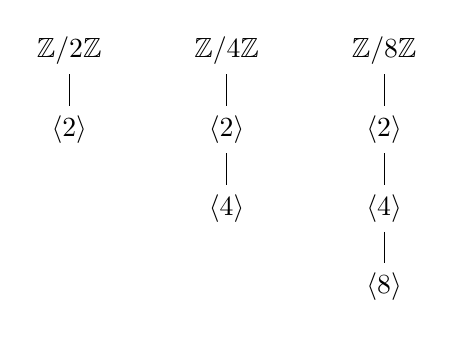
\begin{tikzpicture}
                \node (z2z) at (0, 0) {$\intmod[2]$};
                \node (2 z2) at (0, -1) {$\gen2$};
                \draw (z2z) -- (2 z2);

                \node (z4z) at (2, 0) {$\intmod[4]$};
                \node (2 z4) at (2, -1) {$\gen 2$};
                \node (4 z4) at (2, -2) {$\gen 4$};
                \draw (z4z) -- (2 z4) -- (4 z4);

                \node (z8z) at (4, 0) {$\intmod[8]$};
                \node (2 z8) at (4, -1) {$\gen 2$};
                \node (4 z8) at (4, -2) {$\gen 4$};
                \node (8 z8) at (4, -3) {$\gen 8$};
                \draw (z8z) -- (2 z8) -- (4 z8) -- (8 z8);
            \end{tikzpicture}
        \end{center}
        \item The \textbf{Klein 4-group (Vierergruppe)}, $V_4$, is the group of order 4 with each nonidentity element order 2
        \[
        \begin{array}{c|cccc}
            \cdot & 1 & a & b & c \\
            \hline
            1 & 1 & a & b & c \\
            a & a & 1 & c & b \\
            b & b & c & 1 & a \\
            c & c & b & a & 1
        \end{array} \quad \text{and lattice} \quad
        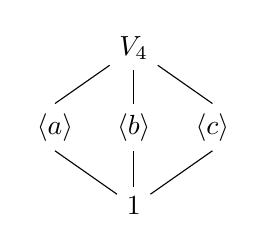
\begin{tikzpicture}[baseline=-0.5ex]
            \node (v4) at (0, 1) {$V_4$};
            \node (a) at (-1, 0) {$\gen a$};
            \node (b) at (0, 0) {$\gen b$};
            \node (c) at (1, 0) {$\gen c$};
            \node (1) at (0, -1) {1};

            \draw (1) -- (a.south);
            \draw (a.north) -- (v4);
            \draw (1) -- (b.south);
            \draw (b.north) -- (v4);
            \draw (1) -- (c.south);
            \draw (c.north) -- (v4);
        \end{tikzpicture}
        \]
        Note that $V_4$ is abelian that is not isomorphic to $Z_4$ since it does not contain elements of order 4.
        \item $S_3$ is the lattice:
        \begin{center}
            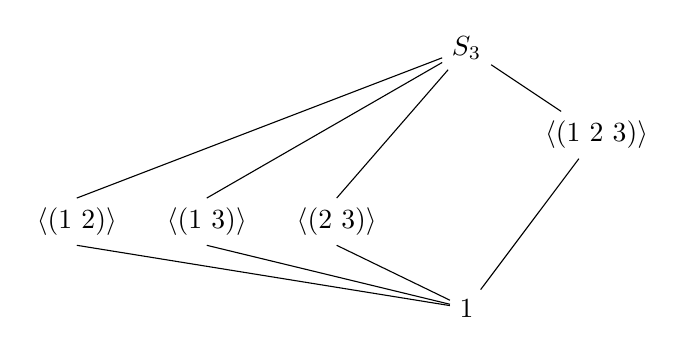
\begin{tikzpicture}[scale = 1.1]
                \node (s3) at (0, 0) {$S_3$};
                \node (12) at (-4.5, -2) {$\gen{(1\ 2)}$};
                \node (13) at (-3, -2) {$\gen{(1\ 3)}$};
                \node (23) at (-1.5, -2) {$\gen{(2\ 3)}$};
                \node (123) at (1.5, -1) {$\gen{(1\ 2\ 3)}$};
                \node (1) at (0, -3) {1};

                \draw (1) -- (12.south);
                \draw (12.north) -- (s3);
                \draw (1) -- (13.south);
                \draw (13.north) -- (s3);
                \draw (1) -- (23.south);
                \draw (23.north) -- (s3);
                \draw (1) -- (123) -- (s3);
            \end{tikzpicture}
        \end{center}
        \item $D_8$ is the lattice:
        \begin{center}
            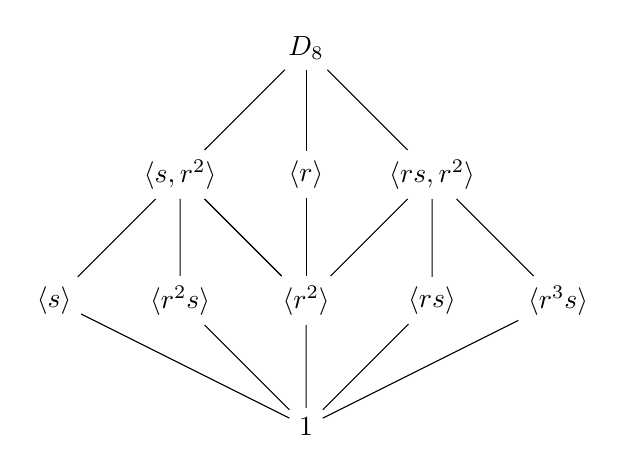
\begin{tikzpicture}[scale=1.6]
                \node (d8) at (0, 0) {$D_8$};
                \node (sr2) at (-1, -1) {$\gen{s, r^2}$};
                \node (r) at (0, -1) {$\gen r$};
                \node (rsr2) at (1, -1) {$\gen{rs, r^2}$};
                \node (s) at (-2, -2) {$\gen s$};
                \node (r2s) at (-1, -2) {$\gen{r^2s}$};
                \node (r2) at (0, -2) {$\gen{r^2}$};
                \node (rs) at (1, -2) {$\gen{rs}$};
                \node (r3s) at (2, -2) {$\gen{r^3s}$};
                \node (1) at (0, -3) {1};

                \draw (1) -- (s) -- (sr2) -- (d8);
                \draw (1) -- (r2s) -- (sr2);
                \draw (1) -- (r2) -- (sr2);
                \draw (1) -- (rs) -- (rsr2) -- (d8);
                \draw (1) -- (r3s) -- (rsr2);
                \draw (r2) -- (r) -- (d8);
                \draw (r2) -- (sr2);
                \draw (r2) -- (rsr2);
            \end{tikzpicture}
        \end{center}
        \item $Q_8$ is the lattice:
        \begin{center}
            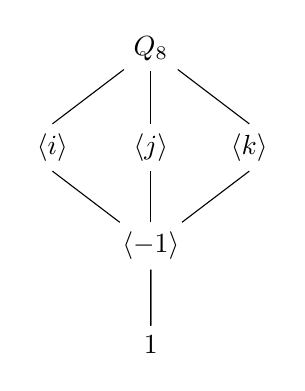
\begin{tikzpicture}[scale=1.25]
                \node (q8) at (0, 0) {$Q_8$};
                \node (i) at (-1, -1) {$\gen i$};
                \node (j) at (0, -1) {$\gen j$};
                \node (k) at (1, -1) {$\gen k$};
                \node (-1) at (0, -2) {$\gen{-1}$};
                \node (1) at (0, -3) {1};

                \draw (1) -- (-1) -- (i.south);
                \draw (i.north) -- (q8);
                \draw (1) -- (-1) -- (j) -- (q8);
                \draw (1) -- (-1) -- (k.south);
                \draw (k.north) -- (q8);
            \end{tikzpicture}
        \end{center}
        \item $D_{16}$ has a lattice that is not a planar graph, or is a graph drawn on a plane without lines crossing. A way of drawing it is
        \begin{center}
            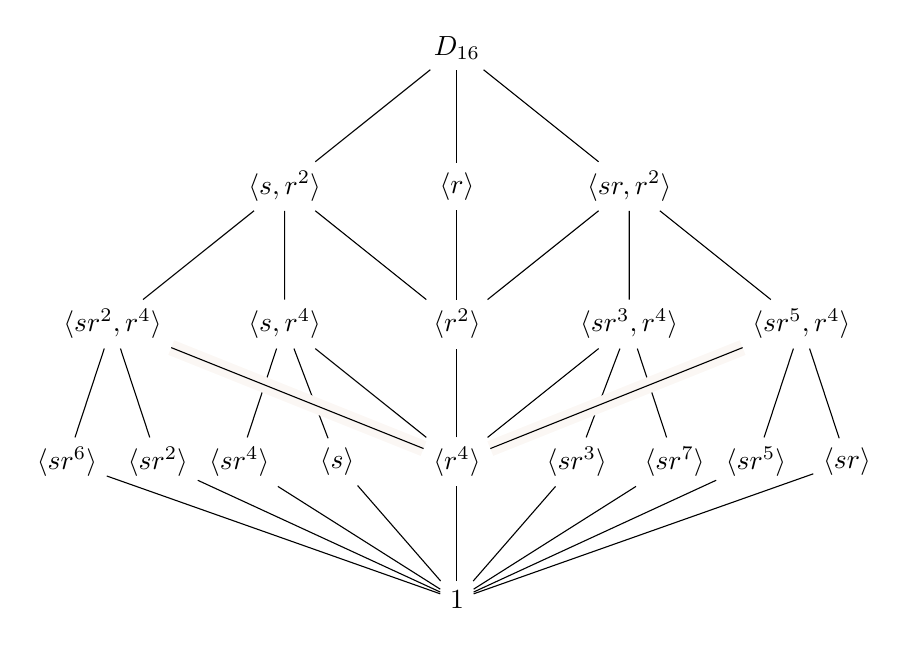
\begin{tikzpicture}[scale=1.75]
                \node (d16) at (0, 0) {$D_{16}$};

                \node (s r2) at (-1.25, -1) {$\gen{s, r^2}$};
                \node (r) at (0, -1) {$\gen r$};
                \node (srr2) at (1.25, -1) {$\gen{sr, r^2}$};

                \node (sr2r4) at (-2.5, -2) {$\gen{sr^2, r^4}$};
                \node (s r4) at (-1.25, -2) {$\gen{s, r^4}$};
                \node (r2) at (0, -2) {$\gen{r^2}$};
                \node (sr3r4) at (1.25, -2) {$\gen{sr^3, r^4}$};
                \node (sr5r4) at (2.5, -2) {$\gen{sr^5, r^4}$};

                \node (sr6) at (-2.83, -3) {$\gen{sr^6}$};
                \node (sr2) at (-2.17, -3) {$\gen{sr^2}$};
                \node (sr4) at (-1.58, -3) {$\gen{sr^4}$};
                \node (s) at (-0.87, -3) {$\gen s$};
                \node (r4) at (0, -3) {$\gen{r^4}$};
                \node (sr3) at (0.87, -3) {$\gen{sr^3}$};
                \node (sr7) at (1.58, -3) {$\gen{sr^7}$};
                \node (sr5) at (2.17, -3) {$\gen{sr^5}$};
                \node (sr) at (2.83, -3) {$\gen{sr}$};

                \node (1) at (0, -4) {1};

                \draw (1) -- (sr6) -- (sr2r4) -- (s r2) -- (d16);
                \draw (1) -- (sr2) -- (sr2r4);
                \draw (1) -- (sr4) -- (s r4) -- (s r2);
                \draw (1) -- (s) -- (s r4);
                \draw (1) -- (r4) -- (r2) -- (r) -- (d16);
                \draw (1) -- (sr3) -- (sr3r4) -- (srr2) -- (d16);
                \draw (1) -- (sr7) -- (sr3r4);
                \draw (1) -- (sr5) -- (sr5r4) -- (srr2);
                \draw (1) -- (sr) -- (sr5r4);
                \draw [preaction={draw, line width=2mm, Tan!10}] (r4) -- (sr2r4);
                \draw (r4) -- (s r4);
                \draw (r4) -- (sr3r4);
                \draw [preaction={draw, line width=2mm, Tan!10}] (r4) -- (sr5r4);
                \draw (r2) -- (s r2);
                \draw (r2) -- (srr2);
            \end{tikzpicture}
        \end{center}
    \end{enumerate}
\end{ex}
\section{Quotient Groups and Homomorphisms}

\subsection{Definitions and Examples} \label{sec3.1}

\defi Let $\phi : G \to H$ be a homomorphism. The \textbf{kernel} of $\phi$ is the set
\[\ker\phi = \{g \in G \mid \phi(g) = 1\}\]
where $1_H$ is the identity of $H$. The \textbf{image} of $\phi$ is the set
\[\im\phi = \{\phi(g) \mid g \in G\}\]

\prop[Homomorphism Properties] \label{prop3.1}
Let $\phi : G \to H$ be a group homomorphism. Then
\begin{enumerate}
    \item $\phi(1_G) = 1_H$, where $1_G$ and $1_H$ are the identities of $G$ and $H$, respectively.
    \item $\phi(g\inv) = \phi(g)\inv$ for every $g \in G$.
    \item $\phi(g^n) = \phi(g)^n$ for every $n \in \z$.
    \item $\ker\phi \leq G$.
    \item $\im\phi \leq H$.
\end{enumerate}

\begin{proofnum}
    \item $\phi(1_G) = \phi(1_G1_G) = \phi(1_G)\phi(1_G)$. By cancellation, $1_H = \phi(1_G)$.
    \item $1_H = \phi(1_G) = \phi(gg\inv) = \phi(g)\phi(g\inv)$ for all $g \in G$. Then $\phi(g)\inv = \phi(g\inv)$.
    \item For $n = 0$, the result is (i). Using induction for $n \in \zp$, use (ii) for $n < 0$.
    \item Note $1_G \in \ker\phi$. Suppose $x, y \in \ker\phi$. Then $\phi(xy\inv) = \phi(x)\phi(y\inv) = 1_H1_H\inv = 1_H$ so that $xy\inv \in \ker\phi$.
    \item Note $1_H \in \im\phi$. Suppose $x, y \in \im\phi$. Then there exists $g, h \in G$ such that $\phi(g) = x$ and $\phi(h) = y$. Then $xy\inv = \phi(g)\phi(h\inv) = \phi(gh\inv)$. Since $gh\inv \in G$, then $xy\inv \in \im\phi$.
\end{proofnum}

\defi Let $\phi : G \to H$ be a homomorphism with kernel $K$. The \textbf{quotient group} $G/K$ is the group whose elements are the fibers of $\phi$ with operation as such: if $X = \phi\inv(a)$ and $Y = \phi\inv(b)$ for $a, b \in H$, then $XY = \phi\inv(ab)$.

\prop[Translates of a Kernel] \label{prop3.2}
Let $\phi : G \to H$ be a homomrphism with kernel $K$. Let $X = \phi\inv(a)$ for $X \in G/K$. Then
\begin{enumerate}
    \item For any $x \in X$, $X = \{xk \mid k \in K\}$.
    \item For any $x \in X$, $X = \{kx \mid k \in K\}$.
\end{enumerate}

\begin{proofnum}
    \item Let $x \in X$, hence $\phi(x) = a$. Let $xK = \set{xk \mid k \in K}$. For any $k \in K$, then $xk \in X$, or $xK \subseteq X$. If $y \in X$, put $k = x\inv y$. Then $k \in K$ so that $y = xk \in xK$, hence $X \subseteq xK$.
    \item Define $Kx = \set{kx \mid k \in K}$. The proof follows similarly as (i), except we set $k = yx\inv$ so that $kx = y \in X$, hence $X \subseteq Kx$.
\end{proofnum}

\defi Let $N \leq G$ and $g \in G$. The \textbf{left coset} and \textbf{right coset} of $N$ in $G$ are the sets
\[gN = \{gn \mid n \in N\}, \quad Ng = \{ng \mid n \in N\}.\]
Elements of a coset are called \textbf{representatives}.

\theo[Coset Multiplication] \label{theo3.3}
Let $G$ be a group with $K$ a kernel of some homomorphism from $G$ to another group. The set of left cosets of $K$ in $G$ with operation
\[aK \circ bK = (ab)K\]
forms the group $G/K$. This operation is well defined in that if $a' \in aK$ and $b' \in bK$, then $a'b' \in abK$, and $a'b'K = abK$. This is also analogously defined for right cosets.
\begin{proof}
    Let $X, Y \in G/K$ with $Z = XY \in G/K$. Then $X, Y, Z$ are left cosets of $K$. Since $K$ is the kernel of a homomorphism, then $X = \phi\inv(a)$ and $Y = \phi\inv(b)$ for $a, b \in H$. Moreover, $Z = \phi\inv(ab)$. Let $x \in X$ and $y \in Y$ so that $\phi(x) = a$ and $\phi(y) = b$. Then $X = xK$ and $Y = yK$. Then $xy \in Z$ if and only if $xy \in \phi\inv(ab)$, or $\phi(x)\phi(y) = ab$, hence $Z = xyK$. Exercise 3.1.2 shows the other direction. Lastly, \autoref{prop3.2} shows that $xK = Kx$ and $yK = Ky$ for every $x, y \in G$.
\end{proof}

\newpage

\note Using similar notation from $\intmod$, we denote $G/K = \bar G$ with $\bar g = gK$ and $\bar g \bar h = \bar{gh}$.

\prop[Set of Cosets is Partition, Equivalency Criterion of Cosets] \label{prop3.4}
Let $N \leq G$. The set of left cosets of $N$ in $G$ form a partition of $G$. Moreover, for all $g, h \in G$, then $gN = hN$ if and only if $h\inv g \in N$. In particular, $gN = hN$ if and only if $g$ and $h$ represent the same coset.

\begin{proof}
    It is clear that $g \in gN$ for every $g \in G$. If $gN \cap hN$ is nonempty, let $k \in gN \cap hN$. Then $k = gn_1 = hn_2$ for $n_1, n_2 \in N$. Note that $g = kn_1\inv = hn_2n_1\inv$ where $n_2n_1\inv \in N$ since $N \leq G$. Then for any $gn \in gN$ for some $n \in N$, we have $gn = hn_2n_1\inv n \in hN$ so that $gN \subseteq hN$. A similar argument shows that $hN \subseteq gN$, hence they are equal, so that the cosets are either distinct or equal.

    The preceding argument shows $gN = hN$ if and only if $g \in hN$, or $g = hn$, or $h\inv g \in N$. Moreover, $h \in gN$ implies that $h$ is a representative of $gN$, so that $hN = gN$ if and only if $g$ and $h$ represent the same coset.
\end{proof}

\prop[Coset Multiplication, Extended] \label{prop3.5}
Let $G$ be a group with $N \leq G$.
\begin{enumerate}
    \item The operation $\cdot$ on the set of left cosets of $N$ in $G$ described by
    \[aN \cdot bN = (ab)N\]
    is well defined if and only if $gng\inv \in N$ for every $g \in G$ and $n \in N$.
    \item Well definedness of the above operation implies that the set of left cosets of $N$ in $G$ forms a group with identity $1N = N$ and inverse of $gN$ given by $(gN)\inv = g\inv N$.
\end{enumerate}

\begin{proofnum}
    \item Suppose the operation is well defined, and let $g \in G$ and $n \in N$. Then $g\inv N = ng\inv N$. Since $1 \in N$, then $ng\inv 1 \in ng\inv N$ so that $ng\inv = g\inv n'$ for some $n' \in N$. Then $gng\inv \in N$.
    
    If $gng\inv \in N$ instead for every $g \in G$ and $n \in N$, let $a, a_0 \in aN$ and $b, b_0 \in bN$ so that $a_0 = an$ and $b_0 = bm$ for some $n, m \in N$. Then
    \[a_0b_0 = (an)(bm) = a(nb)m = a(bn')m\]
    where we note that $nb = b(n')$ for some $n' \in N$ by assumption. Then $a_0b_0 \in abN$ so that $a_0b_0N \cap abN$ is nonempty. By \autoref{prop3.4}, then $a_0b_0N = abN$, hence the operation is well defined.
    \item Trivial verification using the prior proposition and the fact that $G$ is a group.
\end{proofnum}

\defi Let $N \leq G$ for group $G$.
\begin{itemize}
    \item For $n \in N$, the \textbf{conjugate} of $n$ by $g$ is the element $gng\inv$.
    \item The \textbf{conjugate} of $N$ by $g$ is the set $gNg\inv = \{gng\inv \mid n \in N\}$.
    \item We say some $g \in G$ \textbf{normalizes} $N$ if $gNg\inv = N$.
    \item We say $N$ is a \textbf{normal subgroup} of $G$, denoted by $N \nsub G$, if $gNg\inv = N$ for every $g \in G$. Equivalently, $N$ is normal if and only if every element of $G$ normalizes $N$.
\end{itemize}

\theo[Characterizations of Normal Subgroups] \label{theo3.6}
Let $G$ be a group with $N \leq G$. Then the following are equivalent:
\begin{enumerate}
    \item $N \nsub G$,
    \item $N_G(N) = G$,
    \item $gN = Ng$ for every $g \in G$,
    \item the operation on left cosets of $N$ in $G$ described in \autoref{prop3.5} makes the set of left cosets into a group,
    \item $gNg\inv \subseteq N$ for every $g \in G$.
\end{enumerate}

\begin{proof}
    \leavevmode
    \begin{itemize}
        \item (i) if and only if (ii) by definition of normality and normalizer.
        \item (ii) if and only if (iii), since $gNg\inv = N$ implies $gN = Ng$ for every $g \in G$.
        \item (iii) implies (iv) by \autoref{prop3.5}.
        \item (iv) implies (v), as well definedness of the operation implies $gng\inv \in N$ for every $g \in G$ and $n \in N$ by \autoref{prop3.5}.
        \item (v) implies (i), because $g\inv Ng \subseteq N$ in particular, hence $N \subseteq gNg\inv \subseteq N$ so that $gNg\inv = N$ for every $g \in G$.
    \end{itemize}
\end{proof}

\prop[Normal Subgroup Are Kernels] \label{prop3.7}
$N \nsub G$ if and only if $N = \ker\phi$ for some homomorphism $\phi$ on $G$.
\begin{proof}
    If $N \nsub G$, let $\pi : G \to G/N$ be the map
    \[\pi(g) = gN, \quad g \in G\]
    It is clear that $\pi$ is a homomorphism. Moreover, $\pi(g) = 1N$ when $gN = N$, or $g \in N$, hence $\ker\pi = N$.

    If $N$ is instead a kernel of some homomorphism, then $gN = Ng$ for $g \in G$ by \autoref{prop3.2}. Then $N \nsub G$ by \autoref{theo3.6}.
\end{proof}

\defi For $N \nsub G$, then the homomorphism $\pi : G \to G/N$ given by $\pi(g) = gN$ is called the \textbf{natural projection homomorphism} from $G$ to $G/N$. Moreover, for $\bar H \leq G/N$, the set $\pi\inv(\bar H)$ is the \textbf{complete preimage} of $\bar H$ in $G$.

\note We claim quotient groups of cyclic groups are cyclic. Let $G = Z_n$ for some $n \in \zp$ with $g \in G$ such that $\gen g = G$. For some $N \leq G$, we know $N = \gen{g^d}$ for smallest positive integer $d$ such that $g^d \in N$. Note that $g^\alpha N = (gN)^\alpha$ for every $\alpha \in \z$ by Exercise 3.1.4, hence $G/N = \gen{gN}$. By Exercise 3.1.5, we know $|gN| = d$, and $d = |G|/|N|$ by \autoref{prop2.5}, so that $G/N \cong Z_d$.
\newpage

\subsection{More on Cosets and Lagrange's Theorem} \label{sec3.2}

\theo[Lagrange's Theorem] \label{theo3.8}
Let $G$ be a finite group with $H \leq G$. Then $|H|$ divides $|G|$. Also, the number of left cosets of $H$ in $G$ is $|G|/|H|$.
\begin{proof}
    Let $|H| = n$ and let $k$ be the number of left cosets of $H$ in $G$. \autoref{prop3.4} shows that these cosets partition $H$, and the map $H \to gH$ given by $h \mapsto gH$ is a bijection for every $g \in G$, hence each coset has $n$ elements. Since the cosets partition $G$, then $|G| = kn$, so that $n$ divides $|G|$ and the number of left cosets is $k = |G|/n$.
\end{proof}

\defi Let $G$ be a (possibly infinite) group with $H \leq G$. The \textbf{index} of $H$ in $G$ is the number of left cosets of $H$ in $G$, denoted by $|G : H|$.

\cor[Element Order Divides Group Order] \label{cor3.9}
Let $G$ be a finite group and let $g \in G$. Then the order of $g$ divides the order of $G$. In particular, $g^{\abs G} = 1$.
\begin{proof}
    \autoref{prop2.2} shows that $\abs g = \abs{\gen x}$. Then the first part follows by using Lagrange's Theorem on $H = \gen g$. Since $\abs G$ is a multiple of $\abs g$, the second part follows.
\end{proof}

\cor[Prime Order Implies Cyclic] \label{cor3.10}
Let $G$ be a group of prime order. Then $G \cong Z_p$ for some prime $p$.
\begin{proof}
    For non-identity $g \in G$, then $\gen g \leq G$ is nontrivial, hence $\gen g = G$ by the primality of $|G|$. Then $G$ is cyclic, and $G \cong Z_{|G|}$ by \autoref{theo2.4}.
\end{proof}

\note We claim $H \nsub G$ when $|G : H| = 2$. For $g \in G - H$, then $G/H = \set{1H, gH} = \set{H1, Hg}$. Since $H = 1H = H1$, then $gH = G - H = Hg$, hence $H \nsub G$ by \autoref{theo3.6}.

\theo[Cauchy's Theorem] \label{theo3.11}
Let $G$ be finite with prime $p$ dividing $|G|$. Then there exists $g \in G$ where $|g| = p$.

\theo[Sylow] \label{theo3.12}
Let $G$ be finite with $|G| = p^nm$ such that $p$ is prime and $p \nmid m$. Then there exists $H \leq G$ such that $|H| = p^n$.

\defi Let $H, K \leq G$. The \textbf{subgroup product} of $H$ and $K$ is the set
\[HK = \{hk \mid h \in H, k \in K\}\]

\prop[Cardinality of Subgroup Product] \label{prop3.13}
Let $H$ and $K$ be subgroups of a finite group $G$. Then
\[|HK| = \frac{|H||K|}{|H \cap K|}\]
\begin{proof}
    Observe $HK$ is a union of left cosets of $K$. To find the number of distinct left cosets of the form $hK$ for $h \in H$, observe that $h_1K = h_2K$ for some $h_1, h_2 \in H$ if and only if $h_2\inv h_1 \in K$, or $h_2\inv h_1 \in H \cap K$. Then the number of distinct left cosets of $K$ in $HK$ is $|H : H \cap K| = |H|/|H \cap K|$. The result follows by noting that each coset has $|K|$ elements.
\end{proof}

\prop[Characterization of Subgroup Product as a Subgroup] \label{prop3.14}
If $H, K \leq G$, then $HK \leq G$ if and only if $HK = KH$.
\begin{proof}
    If $HK \leq G$, we have $KH \subseteq HK$ from $H, K \leq HK$. For $hk \in HK$, then $hk = (h_0k_0)\inv = k_0\inv h_0\inv \in KH$ for some $h_0 \in H$ and $k_0 \in K$, hence $HK \subseteq KH$.

    If $HK = KH$, let $a, b \in HK$ with $a = h_1k_1, b = h_2k_2$ for $h_i \in H$ and $k_i \in K$. Then $ab\inv = h_1k_1k_2\inv h_2\inv \in HK$. Since $KH = HK$, $(k_1k_2\inv) h_2\inv = h_3k_3$ for some $h_3 \in H$ and $k_3 \in K$, hence $ab\inv = h_1h_3k_3 \in HK$, or $HK \leq G$.
\end{proof}

\cor[Normalizing Criterion for Subgroup Products] \label{cor3.15}
Let $H, K \leq G$ with $H \leq N_G(K)$. Then $HK \leq G$. In particular, $K \nsub G$ implies $HK \leq G$ for every $H \leq G$.

\begin{proof}
    Observe $khk\inv in K$ for all $h \in H$ and $k \in K$ by assumption. Then $hk = (hkh\inv)h \in KH$, and $kh = h(h\inv kh) \in HK$ for all $h \in H$ and $k \in K$, hence $HK = KH$. By \autoref{prop3.14}, then $HK \leq G$.
\end{proof}

\defi Let $A \subseteq N_G(K)$ or $C_G(K)$. Then $A$ \textbf{normalizes}, or \textbf{centralizes} $K$, respectively.

\newpage

\subsection{The Isomorphism Theorems} \label{sec3.3}

\theo[The First Isomorphism Theorem] \label{theo3.16}
If $\phi : G \to H$ is a group homomorphism, then $\ker\phi \nsub G$ and $G/\ker\phi \cong \phi(G)$.
\begin{proof}
    Note that $\ker\phi \nsub G$ by \autoref{prop3.7}. Consider the map
    \[\psi : G/\ker\phi \to \phi(G), \quad g\ker\phi \mapsto \phi(g),\]
    and also observe that $\phi = \psi \circ \pi$ where $\pi$ is the natural projection homomorphism. To show that $\psi$ is well defined, observe that $g\ker\phi = h\ker\phi$ implies $h\inv g \in \ker\phi$, or $\phi(h) = \phi(g)$. The backwards shows injectivity, and surjectivity is clear by definition of $\phi(G)$. A composition of homomorphisms is a homomorphism, hence $\psi$ is an isomorphism from $G/\ker\phi$ to $\phi(G)$.
\end{proof}

\cor[Consequences of the First Isomorphism Theorem] \label{cor3.17}
Let $\phi : G \to H$ be a group homomorphism. Then
\begin{enumerate}
    \item $\phi$ is injective if and only if $\ker\phi = 1$, and
    \item $|G : \ker\phi| = |\phi(G)|$.
\end{enumerate}

\begin{proofnum}
    \item If $\phi$ is injective, then $\phi(g) = 1$ implies $g = 1$. Conversely, a trivial kernel implies for any $g, h \in G$ such that $\phi(g) = \phi(h)$ that $\phi(h\inv g) = 1$, hence $h\inv g = 1$ or $g = h$.
    \item By the First Isomorphism Theorem, then $G/\ker\phi \cong \phi(G)$, so that $|G : \ker\phi| = |G/\ker\phi| = |\phi(G)|$.
\end{proofnum}

\theo[The Second (Diamond) Isomorphism Theorem] \label{theo3.18}
Let $G$ be a group with $A, B \leq G$ and $A \leq N_G(B)$. Then $AB \leq G$, $B \nsub AB$, $A \cap B \nsub A$, and $AB/B \cong A/A \cap B$. A diagram of the subgroup lattice is as follows:
\begin{center}
    \begin{tikzpicture}[scale=1.1]
        \node (G) at (0, 0) {$G$};
        \node (AB) at (0, -1) {$AB$};
        \node (A) at (-1, -2) {$A$};
        \node (B) at (1, -2) {$B$};
        \node (AintB) at (0, -3) {$A \cap B$};
        \node (1) at (0, -4) {$1$};

        \draw (1) -- (AintB) -- (A) -- (AB) -- (G);
        \draw (AintB) -- (B) -- (AB);
    \end{tikzpicture}
\end{center}

\begin{proof}
    \autoref{cor3.15} shows that $AB \leq G$. Also, $AB \leq N_G(B)$, or $B \nsub AB$. Consider $\pi |_A : AB \to AB/B$. Then $\ker\pi|_A$ consists of elements $a \in A$ such that $aB = B$, or $a \in B$, hence $a \in A \cap B$. By the First Isomorphism Theorem, then $A \cap B \nsub A$ and $A/A \cap B \cong AB/B$.
\end{proof}

\theo[The Third Isomorphism Theorem] \label{theo3.19}
Let $G$ be a group with $N_1 \nsub G$ and $N_2 \nsub G$ such that $N_1 \leq N_2$. Then $N_2/N_1 \nsub G/N_1$ and
\[(G/N_1)/(N_2/N_1) \cong G/N_2.\]
\begin{proof}
    It is clear that $N_2/N_1 \nsub G/N_1$ by $N_2 \nsub G$. The map
    \[\phi : G/N_1 \to G/N_2, \quad gN_1 \mapsto gN_2\]
    is well defined, since $N_1 \leq N_2$. It is easy to see that $\phi$ is a surjective homomorphism. Moreover, $\phi(gN_1) = N_2$ if and only if $gN_2 = N_2$, or $g \in N_2$, hence $\ker\phi = N_2/N_1$. The First Isomorphism Theorem finishes the proof.
\end{proof}

\theo[The Fourth (Lattice) Isomorphism Theorem] \label{theo3.20}
Let $G$ be a group with $N \nsub G$. Then every subgroup of $\bar G$ is of the form $\bar A$ for some $A \leq G$ with $N \leq A$, and $A \mapsto \bar A$ is a bijection from the set of subgroups of $G$ containing $N$ to the set of subgroups of $\bar G$. This bijection has the following properties:
\begin{enumerate}
    \item $A \leq B$ if and only if $\bar A \leq \bar B$,
    \item $A \leq B$ implies $[B : A] = [\bar B : \bar A]$,
    \item $\bar{\gen{A, B}} = \gen{\bar A, \bar B}$,
    \item $\bar{A \cap B} = \bar A \cap \bar B$,
    \item $A \nsub G$ if and only if $\bar A \nsub \bar G$.
\end{enumerate}

\begin{proof}
    See Exercise 3.3.2.
\end{proof}

\note A criterion to define homomorphisms on quotient groups is requiring that the kernel of the homomorphism contains the normal subgroup. In particular, if $N \nsub G$ and $\phi : G \to H$ is a homomorphism such that $N \subseteq \ker\phi$, then we define a homomorphism $\psi : G/N \to H$ by $\psi(gN) = \phi(g)$ for $g \in G$. The well definedness of $\psi$ follows from the fact that $gN = hN$ implies $h\inv g \in N \subseteq \ker\phi$, hence $\phi(g) = \phi(h)$. The diagram below commutes, since $\psi \circ \pi = \phi$ where $\pi : G \to G/N$ is the natural projection homomorphism.
\begin{center}
    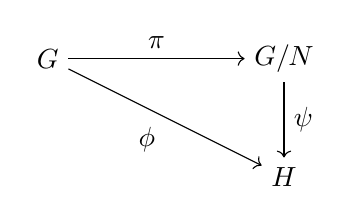
\begin{tikzpicture}
        \node (G) at (0, 0) {$G$};
        \node (GN) at (3, 0) {$G/N$};
        \node (H) at (3, -1.5) {$H$};
        \draw[->] (G) to node[above] {$\pi$} (GN);
        \draw[->] (G) to node[below left] {$\phi$} (H);
        \draw[->] (GN) to node[right] {$\psi$} (H);
    \end{tikzpicture}
\end{center}

\newpage

\subsection{Composition Series and the H\"older Program} \label{sec3.4}

\prop[Cauchy's Theorem for Abelian Groups] \label{prop3.21}
Let $G$ be finite abelian with prime $p$ dividing $|G|$. Then there exists $g \in G$ where $|g| = p$.

\begin{proof}
    Induct on $|G|$. Suppose $|G| > 1$ and $g \in G$ with $g \neq 1$. If $|G| = p$, then $|g| = p$ by Lagrange's. If $|G| > p$ and $p$ divides $|g|$, then $|g| = kp$ for $k \in \zp$, hence $|g^k| = p$ by \autoref{prop2.5}.

    Suppose $p$ does not divide $|g|$, and put $N = \gen g$. Since $G$ is abelian, $N \nsub G$, and Lagrange's shows that $|G/N| = |G|/|N|$ with $|G/N| < |G|$. Since $p$ does not divide $|N|$, then $p$ divides $|G/N|$. By the inductive hypothesis, there exists $\bar h \in G/N$ with $|\bar h| = p$. Note that $h \not\in N$ while $h^p \in N$ since $|\bar h| = p$, $\gen{h^p} \neq \gen h$, or $|h^p| < |h|$. By \autoref{prop2.5}, we have $p$ divides $|h|$. The proof is finished by the first case.
\end{proof}

\defi A (finite/infinite) group $G$ is \textbf{simple} if $G \neq 1$ and the only normal subgroups of $G$ are $1$ and $G$.

\defi Let $G$ be a group with a sequence of subgroups
\[1 = N_0 \leq N_1 \leq \cdots \leq N_{s - 1} \leq N_s = G\]
such that $N_i \nsub N_{i + 1}$ and $N_{i + 1}/N_i$ is simple for every $0 \leq i < s$. Then the sequence is a \textbf{composition series} of $G$. Moreover, the quotient groups $N_{i + 1}/N_i$ are called the \textbf{composition factors} of $G$.

\theo[Jordan--H\"older] \label{theo3.22}
Let $G$ be nontrivial and finite. Then
\begin{enumerate}
    \item $G$ has a composition series, and
    \item the composition factors in a composition series are unique in that if
    \[1 = N_0 \leq N_1 \leq \cdots \leq N_{s - 1} \leq N_s = G, \quad 1 = M_0 \leq M_1 \leq \cdots \leq M_{t - 1} \leq M_t = G\]
    are two composition series of $G$, then $s = t$ and there exists a permutation $\pi$ of $\set{1, 2, \ldots, s}$ such that $N_{i + 1}/N_i \cong M_{\pi(i) + 1}/M_{\pi(i)}$ for all $i$.
\end{enumerate}

\begin{proof}
    See Exercises 3.4.6, 3.4.9, and 3.4.10.
\end{proof}

\defi The \textbf{H\"older Program} is the program:
\begin{enumerate}
    \item Classify all simple groups, and
    \item Use the classification of simple groups to classify all finite groups by the Jordan--H\"older Theorem.
\end{enumerate}

\noindent \textcolor{Plum}{{\large$\heartsuit$} \squad \textsc{Theorem: The Classification of Finite Simple Groups}}

There are 18 infinite families of finite simple groups, and 26 sporadic finite simple groups such that every finite simple group is isomorphic to exactly one of these groups.

\noindent \textcolor{Plum}{{\large$\heartsuit$} \squad \textsc{Theorem: Feit--Thompson}}

Every finite simple group of odd order is isomorphic to $Z_p$ for some prime $p$.

\defi A group $G$ is \textbf{solvable} if there is a chain of subgroups
\[1 = H_0 \nsub H_1 \nsub \cdots \nsub H_{n - 1} \nsub H_n = G\]
such that $H_{i + 1}/H_i$ is abelian for every $0 \leq i < n$.

\noindent \textcolor{Plum}{{\large$\heartsuit$} \squad \textsc{Theorem: Hall's Theorem and its Converse}}

A finite group $G$ is solvable if and only if for every divisor $n$ of $|G|$ such that $\gcd(n, |G|/n) = 1$, there exists a subgroup $H \leq G$ such that $|H| = n$.

\ex We claim for any group $G$ with $N \nsub G$ solvable and $G/N$ solvable, then $G$ is solvable. Let $1 = N_0 \nsub N_1 \nsub \cdots N_n = N$ be a chain of subgroups such that $N_{i + 1}/N_i$ is abelian for every $0 \leq i < n$. Let $\bar 1 = \bar{H_0} \nsub \bar{H_1} \nsub \cdots \nsub \bar{H_m} = G/N$ be a chain of subgroups such that $\bar{H_{i + 1}}/\bar{H_i}$ is abelian for every $0 \leq i < m$. By the Fourth Isomorphism Theorem, there are subgroups $H_i$ with $N \leq H_i$ such that $\bar{H_i} = H_i/N$. The Third Isomorphism Theorem shows that
\[\bar{H_{i + 1}}/\bar{H_i} \cong H_{i + 1}/H_i\]
Then
\[1 = N_0 \nsub N_1 \nsub \cdots N_n = N = H_0 \nsub H_1 \nsub \cdots \nsub H_m = G\]
is a chain of subgroups with abelian successive quotients, hence $G$ is solvable.

\newpage

\subsection{Transpositions and the Alternating Group} \label{sec3.5}

\defi A \textbf{transposition} is a 2-cycle. In particular, any $(a_1\ a_2 \cdots a_k)$ with $k \geq 2$ can be written as a product of $k - 1$ transpositions:
\[(a_1\ a_2 \cdots a_k) = (a_1\ a_k)(a_1\ a_{k - 1}) \cdots (a_1\ a_2)\]

\defi Let $a_1, a_2, \ldots, a_n$ be independent symbols, and consider the \textbf{Vandermonde Polynomial} in $a_1, a_2, \ldots, a_n$ defined by
\[\Delta = \prod_{1 \leq i < j \leq n} (a_i - a_j)\]
Let $\sigma \in S_n$ act on $\Delta$ by permuting the subscripts of $a_i$. Then $\sigma(\Delta) = \pm 1 \Delta$. Define the \textbf{sign} of $\sigma$ to be
\[\ep(\sigma) =
\begin{cases}
    1 & \text{if $\sigma(\Delta) = +1 \Delta$} \\
    -1 & \text{if $\sigma(\Delta) = -1 \Delta$}
\end{cases}\]
An \textbf{even} permutation is when $\ep(\sigma) = 1$, and an \textbf{odd} permutation is when $\ep(\sigma) = -1$.

\prop[Sign is Homomorphism] \label{prop3.23}
The map $\ep : S_n \to \set{\pm 1}$ is a homomorphism, where $\set{\pm 1} \cong Z_2$.
\begin{proof}
    For $\tau, \sigma \in S_n$, we have
    \[(\tau\sigma)(\Delta) = \prod_{1 \leq i < j \leq n}(a_{\tau\sigma(i)} - a_{\tau\sigma(j)})\]
    If $\sigma(\Delta)$ has $k$ factors switched, then $\ep(\sigma) = (-1)^k$. There are $k$ factors of the form $a_{\tau\sigma(i)} - a_{\tau\sigma(j)}$ with $\tau\sigma(i) > \tau\sigma(j)$, and $\tau$ switches these factors if and only if $\tau(i) > \tau(j)$, so that $\ep(\tau\sigma) = (-1)^k\ep(\tau) = \ep(\sigma)\ep(\tau)$.
\end{proof}

\prop[Transpositions are Odd, $\ep$ is Surjective] \label{prop3.24}
\begin{proof}
    Note that $\ep((1\ 2)) = -1$. For any $(i\ j)$ with $1 \leq i < j \leq n$, let $\sigma \in S_n$ such that $\sigma(1) = i$ and $\sigma(2) = j$. Then $\ep((i\ j)) = \ep(\sigma(1\ 2)\sigma\inv) = \ep(\sigma)\ep((1\ 2))\ep(\sigma\inv) = -1$. Moreover, $\ep$ is surjective since $\ep((1\ 2)) = -1$ and $\ep(\id) = 1$.
\end{proof}

\note A useful conjugation formula is $\sigma(i\ j)\sigma\inv = (\sigma(i)\ \sigma(j))$ for $\sigma \in S_n$ and $1 \leq i < j \leq n$.

\defi The \textbf{alternating group} $A_n$ is the set of even permutations in $S_n$, or $\ker\ep$. By the First Isomorphism Theorem, then $A_n \nsub S_n$ and $S_n/A_n \cong Z_2$, hence $|A_n| = n!/2$.

\prop[Odd Permutation If and Only If Odd Number of Even Length Cycles] \label{prop3.25}
A permutation $\sigma$ is odd if and only if the number of cycles of even length in its disjoint cycle decomposition is odd.
\begin{proof}
    For $\sigma \in S_n$ with cycle decomposition $\sigma_1\sigma_2 \cdots \sigma_k$, then $\ep(\sigma) = \ep(\sigma_1)\ep(\sigma_2) \cdots \ep(\sigma_k)$. For $\ep(\sigma) = -1$, there must be an odd number of $\sigma_i$ with $\ep(\sigma_i) = -1$, or an odd number of cycles of even length in the cycle decomposition. Conversely, an odd number of cycles of even length in the cycle decomposition implies $\ep(\sigma) = -1$.
\end{proof}

\ex We claim the subgroup lattice of $A_4$ is as follows:
\begin{center}
    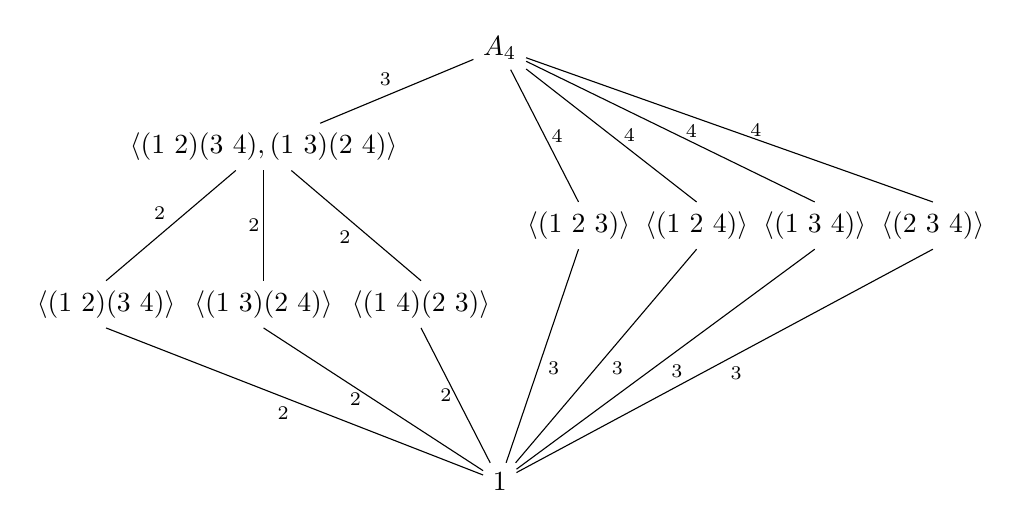
\begin{tikzpicture}
        \node (a4) at (0, 0.25) {$A_4$};

        \node (v4) at (-3, -1) {$\gen{(1\ 2)(3\ 4), (1\ 3)(2\ 4)}$};

        \node (123) at (1, -2) {$\gen{(1\ 2\ 3)}$};
        \node (124) at (2.5, -2) {$\gen{(1\ 2\ 4)}$};
        \node (134) at (4, -2) {$\gen{(1\ 3\ 4)}$};
        \node (234) at (5.5, -2) {$\gen{(2\ 3\ 4)}$};

        \node (1234) at (-5, -3) {$\gen{(1\ 2)(3\ 4)}$};
        \node (1324) at (-3, -3) {$\gen{(1\ 3)(2\ 4)}$};
        \node (1423) at (-1, -3) {$\gen{(1\ 4)(2\ 3)}$};

        \node (1) at (0, -5.25) {1};

        \draw (1) -- (1234.south) node [midway, below left=-2pt] {\scriptsize 2};
        \draw (1234.north) -- (v4) node [midway, above left=-2pt] {\scriptsize 2} -- (a4) node [midway, above left=-2pt] {\scriptsize 3};
        \draw (1) -- (1324.south) node [midway=, left=1pt] {\scriptsize 2};
        \draw (1324.north) -- (v4) node [midway, left=-2pt] {\scriptsize 2};
        \draw (1) -- (1423.south) node [midway, left=-2pt] {\scriptsize 2};
        \draw (1423.north) -- (v4) node [midway, below left=-2pt] {\scriptsize 2};
        \draw (1) -- (123.south) node [midway, below right=-2pt] {\scriptsize 3};
        \draw (123.north) -- (a4) node [midway, right=-1pt] {\scriptsize 4};
        \draw (1) -- (124.south) node [midway, below right=-2pt] {\scriptsize 3};
        \draw (124.north) -- (a4) node [midway, right=1pt] {\scriptsize 4};
        \draw (1) -- (134.south) node [midway, below right=-2pt] {\scriptsize 3};
        \draw (134.north) -- (a4) node [midway, right=2pt] {\scriptsize 4};
        \draw (1) -- (234.south) node [midway, below right=-2pt] {\scriptsize 3};
        \draw (234.north) -- (a4) node [midway, right=4pt] {\scriptsize 4};
    \end{tikzpicture}
\end{center}
\section{Group Actions}

\subsection{Group Actions and Permutation Representations} \label{sec4.1}

\note Please recall definitions of group actions, permutation representations, kernels, stabilizers, and faithful actions from \autoref{sec1.7} and \autoref{sec2.2}.

\ex Let $D_8$ act on $A = \set{\set{1, 3}, \set{2, 4}}$. Let $\b 1 = \set{1, 3}$ and $\b 2 = \set{2, 4}$. A rotation sends one pair to the other, while a reflection fixes both pairs. Hence, the permutation representation afforded by this action is
\[r \mapsto (\b 1\ \b 2), \quad s \mapsto \id,\]
or $\sigma_r = (\b 1\ \b2)$ and $\sigma_s = \id$. Note that $r^2 \mapsto \id$, hence the kernel of the action is $\gen{r^2, s}$.

\prop[Group Actions as Homomorphisms] \label{prop4.1}
For a group $G$ acting on a nonempty set $A$, there exists a bijection between the set of group actions of $G$ on $A$ and the set of homomorphisms from $G$ to $S_A$.
\begin{proof}
    Let $\phi : G \to S_A$, and consider the action of $G$ on $A$ defined by $g \cdot a = \phi(g)(a)$ for all $g \in G$ and $a \in A$. Clearly, the kernel of this action is $\ker\phi$, and the permutation representation afforded by this action is $\phi$ itself. 
\end{proof}

\defi Let $G$ be a group. Then a \textbf{permutation representation} of $G$ is a homomorphism of $G$ into $S_A$ for nonempty $A$. A given action of $G$ on $A$ \textbf{affords} or \textbf{induces} the associated permutation representation.

\begin{prop}[Orbit-Stabilizer Theorem]
    \label{prop4.2}
    Let $G$ be a group acting on the nonempty set $A$. Then the relation on $A$ defined by
    \[a \sim b \quad \text{if and only if} \quad a = g \cdot b~\text{for some $g\in G$}\]
    is an equivalence relation. Moreover, for each $a \in A$, the size of the orbit of $a$ is given by $|G : G_a|$, the index of the stabilizer of $a$ in $G$.
    \begin{proof}
        Let $a, b, c \in G$. Reflexivity is trivial. If $a \sim b$, or $a = g \cdot b$ for $g \in G$, then $g\inv \cdot a = 1 \cdot b$, hence $b \sim a$. If $a \sim b$ and $b \sim c$ with $a = g \cdot b$ and $b = h \cdot c$ for $g, h \in G$, then $a = (gh) \cdot c$. Hence, $\sim$ is an equivalence relation.

        Consider $[a]$. Let $b = g \cdot a \in [a]$. Then $g [a]$ is a left coset of $G_a$ in $G$. Define the map
        \[\psi : [a] \to G/G_a, \quad g \cdot a \mapsto gG_a.\]
        To see that $\psi$ is well defined and injective, note that $g \cdot a = h \cdot a$ if and only if $gG_a = hG_a$. Surjectivity is clear.
    \end{proof}
\end{prop}

\defi Let $G$ act on nonempty $A$.
\begin{enumerate}
    \item The \textbf{orbit} of $a \in A$ is the equivalence class $[a]$ in \autoref{prop4.2}.
    \item The action is \textbf{transitive} if there is only one orbit, i.e., for every $a, b \in A$, there exists some $g \in G$ such that $g \cdot a = b$.
\end{enumerate}

\ex $S_n$ acts on $\set{1, 2, \ldots, n}$ transitively by the natural action.

\note To see that elements of $S_n$ have unique cycle decompositions, let $A = \set{1, 2, \ldots, n}$, $\sigma \in S_n$, and $G = \gen\sigma$. Let $G$ act on $A$, so by \autoref{prop4.2}, $A$ is partitioned into a unique set of disjoint orbits. Let $\oo$ be an orbit with some $a \in \oo$. The proof of \autoref{prop4.2} shows that the cosets of $G_a$ in $G$ are in bijection with elements of $\oo$ explicitly by
\[\psi : \oo \to G/G_a, \quad \sigma^k \cdot a \mapsto \sigma^k G_a.\]
Note that $G/G_a$ is cyclic with order $d = |G : G_a| = |\oo|$, where $d$ is smallest positive integer such that $\sigma^d \in G_a$. Thus, the distinct cosets of $G_a$ in $G$ are
\[\set{G_a, \sigma G_a, \sigma^2 G_a, \ldots, \sigma^{d-1}G_a},\]
and the elements of $\oo$ are
\[\set{a, \sigma \cdot a, \sigma^2 \cdot a, \ldots, \sigma^{d-1} \cdot a}.\]
Then $\sigma$ acts on $\oo$ as a $d$-cycle, and the cycle decomposition of $\sigma$ is obtained by considering all distinct orbits of $G$ on $A$. Since the orbits are unique, the cycle decomposition of $\sigma$ is unique up to the order of the cycles.
\newpage

\subsection{Groups Acting on Themselves by Left Multiplication---Cayley's Theorem} \label{sec4.2}

\note For finite $G$, enumerate the elements as $g_1, \ldots, g_n$. A permutation $\sigma_g$ for $g \in G$ is then given by
\[\sigma_g(i) = j \quad \text{if and only if} \quad gg_i = g_j,\]
with different labelling of the elements of $G$ giving different permutations. 

\ex Label $V_4 = \set{1, a, b, c}$ as $1, 2, 3, 4$ respectively. Computing $\sigma_a$, we see
\begin{align*}
    a \cdot 1 = a & \implies \sigma_a(1) = 2, \\
    a \cdot a = 1 & \implies \sigma_a(2) = 1, \\
    a \cdot b = c & \implies \sigma_a(3) = 4, \\
    a \cdot c = b & \implies \sigma_a(4) = 3,
\end{align*}
hence $\sigma_a = (1\ 2)(3\ 4)$. Similarly, we have $\sigma_b = (1\ 3)(2\ 4)$ and $\sigma_c = (1\ 4)(2\ 3)$.

\ex Let $H \leq G$ for group $G$, and let $A = G/H$. We may define $G$ to act on $A$ by left multiplication via the action
\[g \cdot (xH) = (gx)H \quad \text{for all $g, x \in G$}.\]
Moreover, if $|G : H|$ is finite, we may similarly enumerate them as previously done.

\theo[Properties of the Coset Action] \label{theo4.3}
Let $G$ be a group with $H \leq G$, and let $G$ act on $A = G/H$ by left multiplication. Let $\pi_H$ be the associated permutation representation afforded by this action. Then
\begin{enumerate}
    \item $G$ acts transitively on $A$,
    \item $G_{1H} = H$, and
    \item $\ker\pi_H = \bigcap_{g \in G} gHg\inv$, and $\ker\pi_H$ is the largest normal subgroup of $G$ contained in $H$.
\end{enumerate}

\begin{proofnum}
    \item Let $g_1H, g_2H \in A$, and put $g = g_2g_1\inv$. Then $g \cdot (g_1H) = g_2H$.
    \item By definition, $G_{1H} = \set{g \in G \mid g \cdot 1H = 1H} = \set{g \in G \mid gH = H} = H$.
    \item By definition, $g \in \ker\pi_H$ when $gxH = xH$, or $x\inv gxH = H$, hence $g \in xHx\inv$ for all $x \in G$. Clearly, $\ker\pi_H \nsub G$ and $\ker\pi_H \leq H$. Let $N \nsub G$ such that $N \leq H$. Then $N = xNx\inv \leq xHx\inv$ for all $x \in G$. It follows that $\ker\pi_H$ is the largest normal subgroup of $G$ contained in $H$.
\end{proofnum}

\cor[Cayley's Theorem] \label{cor4.4}
Every group is isomorphic to a subgroup of a symmetric group.
\begin{proof}
    Use $H = 1$ in \autoref{theo4.3}. Then $\ker\pi_H = 1$, so that $\pi_H$ is injective, and $G$ is isomorphic to the subgroup $\pi_H(G)$ of $S_{G/H} = S_G$.
\end{proof}

\cor[Subgroups of Smallest Prime Index are Normal] \label{cor4.5}
Let $|G| = n < \infty$, and let $p$ be the smallest prime dividing $n$. Then every subgroup of index $p$ in $G$ is normal.

\begin{proof}
    Let $H \leq G$ with $|G : H| = p$. Let $\pi_H$ be the permutation afforded by $G$ acting on $G/H$ by left multiplication, let $K = \ker\pi_H$, and put $|H : K| = k$. Then $|G : K| = |G : H||H : K| = pk$. By the First Isomorphism Theorem, $G/K \cong \pi_H(G) \leq S_{G/H} = S_p$. Lagrange's shows that $pk \mid p!$, or $k \mid (p - 1)!$. Since $p$ is the smallest prime dividing $n$, then $k = 1$, so that $H = K \nsub G$.
\end{proof}

\newpage

\subsection{Groups Acting on Themselves by Conjugation---The Class Equation} \label{sec4.3}

\defi 
\begin{itemize}
    \item Let $g, h \in G$. Then $g$ and $h$ are \textbf{conjugate} in $G$ if there exists some $x \in G$ such that $h = xgx\inv$. The equivalence classes of this relation are the \textbf{conjugacy classes} of $G$.
    \item Let $G$ act on $\pp(G)$. For $S, T \in \pp(G)$, we say $S$ and $T$ are \textbf{conjugate} in $G$ if there exists some $x \in G$ such that $T = xSx\inv$, generalizing the previous definition of conjugacy for elements of $G$.
\end{itemize}

\prop[Conjugation Under Orbit-Stabilizer Theorem] \label{prop4.6}
The number of conjugates of $S \subseteq G$ in $G$ is $|G : N_G(S)|$. Moreover, the number of conjugates of $g \in G$ is $|G : C_G(g)|$.

\begin{proof}
    Note that $G_S = \set{g \in G \mid gSg\inv = S} = N_G(S)$, and $N_G(g) = C_G(g)$ for any $g \in G$.
\end{proof}

\theo[The Class Equation] \label{theo4.7}
Let $G$ be finite with $g_1, g_2, \ldots, g_s$ be representatives of distinct conjugacy classes of $G$ not in $Z(G)$. Then
\[|G| = |Z(G)| + \sum_{i=1}^s |G : C_G(g_i)|.\]
\begin{proof}
    Note that each $z \in Z(G)$ has conjugacy class $\set z$, and each $g_i$ has conjugacy class of size $|G : C_G(g_i)|$. Since the conjugacy classes of $G$ partition $G$, the class equation follows.
\end{proof}

\ex Observe $\gen g \leq C_G(g)$ for any $g \in G$. In $G = Q_8$, we know $\gen i \leq C_G(i) \leq G$. However, $i \not\in Z(G)$, so that $C_G(i)$ is a proper subgroup of $G$. Since $|G : \gen i| = 4$, it follows that $C_G(i) = \gen i$. Hence, the conjugacy class of $i$ has size $|G : C_G(i)| = 2$, and the conjugates of $i$ are itself and $-i = jij\inv$. The conjugacy classes for $j$ and $k$ are similar, hence the conjugacy classes of $Q_8$ are
\[\set 1, \quad \set{-1}, \quad \set{\pm i}, \quad \set{\pm j}, \quad \set{\pm k}\]
with sizes 1, 1, 2, 2, and 2, respectively. The class equation for $Q_8$ is then $|Q_8| = 2 + 2 + 2 + 2 = 8$.

\theo[Prime Power Order Implies Nontrivial Center] \label{theo4.8}
Let $p$ be prime with $|P| = p^n$ for $n \geq 1$. Then $Z(P)$ is nontrivial.
\begin{proof}
    The class equation gives
    \[|P| = |Z(P)| + \sum_{i=1}^m |P : C_P(g_i)|,\]
    with representatives $g_1, g_2, \ldots, g_m$ of distinct conjugacy classes. Since $C_P(g_i) \neq P$, each $|P : C_P(g_i)|$ is a power of $p$, hence $|Z(P)|$ is divisible by $p$, so that $Z(P)$ is nontrivial.
\end{proof}

\cor[Classification of Groups of Order $p^2$] \label{cor4.9}
If $|P| = p^2$ for prime $p$, then $P$ is abelian. More precisely, $P \cong Z_{p^2}$ or $P \cong Z_p \times Z_p$.
\begin{proof}
    \autoref{theo4.8} implies $Z(P) \neq 1$, hence $P/Z(P)$ is cyclic and $P$ is abelian. If $x \in P$ with $|x| = p^2$, then $P = \gen x$, so assume no element of $P$ has order $p^2$, hence has order $p$. Consider nonidentity $a \in P$ with $b \in P - \gen a$. We have $\gen a < \gen{a, b}$ strictly by construction, hence $\gen{a, b} = P$. Observe $\gen a \times \gen b = Z_p \times Z_p$, and the map $(a^m, b^n) \mapsto a^mb^n$ is clearly an isomorphism from $\gen a \times \gen b$ to $P$.
\end{proof}

\prop[Conjugation in $S_n$] \label{prop4.10}
Let $\sigma, \tau \in S_n$. If $\sigma$ has cycle decomposition
\[\sigma = (a_1\ a_2 \cdots a_{\ell_1})(b_1\ b_2 \cdots b_{\ell_2}) \cdots\]
then the cycle decomposition of $\tau\sigma\tau\inv$ is
\[\tau\sigma\tau\inv = (\tau(a_1)\ \tau(a_2) \cdots \tau(a_{\ell_1}))(\tau(b_1)\ \tau(b_2) \cdots \tau(b_{\ell_2})) \cdots\]
\begin{proof}
    If $\sigma(i) = j$, it is clear that $\tau\sigma\tau\inv(\tau(i)) = \tau(j)$.
\end{proof}

\defi Let $\sigma \in S_n$ be the product of disjoint cycles with lengths $\ell_1, \ell_2, \ldots, \ell_k$, such that $\ell_1 \leq \ell_2 \leq \cdots \leq \ell_k$. Then the \textbf{cycle type} of $\sigma$ is the $k$-tuple $(\ell_1, \ell_2, \ldots, \ell_k)$.

\defi A \textbf{partition} of $n \in \zp$ is a nondecreasing sequence of positive integers with sum $n$.

\prop[Conjugacy Criterion in $S_n$] \label{prop4.11}
$\sigma, \tau \in S_n$ are conjugate if and only if they have the same cycle type. Moreover, the number of conjugacy classes of $S_n$ is the number of partitions of $n$.
\begin{proof}
    \autoref{prop4.10} shows that conjugate permutations have the same cycle type. Conversely, if $\sigma$ and $\tau$ have the same cycle type, then we may write
    \[\sigma = (a_1\ a_2 \cdots a_{\ell_1})(b_1\ b_2 \cdots b_{\ell_2}) \cdots, \quad \tau = (c_1\ c_2 \cdots c_{\ell_1})(d_1\ d_2 \cdots d_{\ell_2}) \cdots\]
    Then $\alpha \in S_n$ defined by $\alpha(a_i) = c_i$ for $1 \leq i \leq \ell_1$, $\alpha(b_i) = d_i$ for $1 \leq i \leq \ell_2$, and so on, satisfies $\alpha\sigma\alpha\inv = \tau$.

    The conjugacy classes of $S_n$ are in bijection with the cycle types of elements of $S_n$, which are in bijection with the partitions of $n$, hence the second assertion follows.
\end{proof}

\ex For an $m$-cycle $\sigma \in S_n$, we claim the number of conjugates of $\sigma$ is
\[\frac{|S_n|}{|C_{S_n}(\sigma)} = \frac{n!}{m(n - m)!} = \frac{n(n - 1) \cdots (n - m + 1)}{m}\]
Note $\sigma$ commutes with its powers, and commutes with the $(n - m)!$ permutations of the remaining $n - m$ integers, hence $|C_{S_n}(\sigma)| = m(n - m)!$.

\note If $H \nsub G$, then for any conjugacy class $\cc$ of $G$, either $\cc \subseteq H$ or $\cc \cap H = \emptyset$: if $g \in \cc \cap H$, then $xgx\inv \in H$ for all $x \in G$, hence $\cc \subseteq H$.

\theo[$A_5$ is Simple] \label{theo4.12}
\begin{proof}
    We know the representatives of the even permutations are of the form
    \[\id, (1\ 2\ 3), (1\ 2\ 3\ 4\ 5), (1\ 2)(3\ 4).\]
    \begin{itemize}
        \item $\id$ is its own conjugacy class with size 1.
        \item $C_{A_5}((1\ 2\ 3)) = \gen{(1\ 2\ 3)}$ has order 3, so the conjugacy class of $(1\ 2\ 3)$ has size $60/3 = 20$. All 3-cycles are conjugate in $A_5$ since they have the same cycle type.
        \item $C_{A_5}((1\ 2\ 3\ 4\ 5)) = \gen{(1\ 2\ 3\ 4\ 5)}$ has order 5, so the conjugacy class of $(1\ 2\ 3\ 4\ 5)$ has size $60/5 = 12$. However, there are 24 5-cycles in $A_5$, so there are two conjugacy classes of 5-cycles in $A_5$.
        \item All odd-order elements have been accounted for, hence the remaining 15 are order 2 with cycle type $(2, 2)$. It is easy to verify that $C_{A_5}((1\ 2)(3\ 4))$ has order 4, so the conjugacy class of $(1\ 2)(3\ 4)$ has size $60/4 = 15$.
    \end{itemize}
    The class equation for $A_5$ is then
    \[60 = 1 + 20 + 12 + 12 + 15.\]
    By the previous note, a nontrivial normal subgroup of $A_5$ must be the union of some of the nontrivial conjugacy classes, but no such union has size dividing 60, hence $A_5$ is simple.
\end{proof}

\defi A \textbf{right group action} can be defined analogously as a map from $A \times G$ to $A$, denoted by $a \cdot g$ for $a \in A$ and $g \in G$, such that
\begin{enumerate}
    \item $a \cdot 1 = a$ for all $a \in A$, and
    \item $(a \cdot g) \cdot h = a \cdot (gh)$ for all $a \in A$ and $g, h \in G$.
\end{enumerate}

\note Conjugation is typically written as a right group action: $a^g = g\inv a g$ for $a, g \in G$. Similarly, $S^g = g\inv S g$ for $S \subseteq G$ and $g \in G$.

\note If we are given a left group action of $G$ on $A$, we can define a right group action of $G$ on $A$ by $a \cdot g = g\inv \cdot a$ for all $a \in A$ and $g \in G$.

\newpage

\subsection{Automorphisms} \label{sec4.4}

\defi An isomorphism from a group $G$ to itself is an \textbf{automorphism}. The set of automorphisms of $G$ is denoted by $\aut(G)$.

\prop[Conjugation on Normal Subgroups] \label{prop4.13}
Let $H \nsub G$. Let $G$ act on $H$ by conjugation. Then $G$ acts on conjugation on $H$ by automorphisms, defined as
\[g \cdot h \mapsto ghg\inv, \quad g \in G, h \in H.\]
Each conjugation by $g$ is in $\aut(H)$, and $\pi_H : G \to \aut(H)$ is a homomorphism with kernel $C_G(H)$. In particular, $G/C_G(H)$ is isomorphic to a subgroup of $\aut(H)$.

\begin{proof}
    Let $\phi_g : H \to H$ be defined by $\phi_g(h) = ghg\inv$ for all $h \in H$. Since $H \nsub G$, then $\phi_g$ is well defined. Observe $\phi_g$ has inverse $(\phi_g)\inv = \phi_{g\inv}$, so $\phi_g$ is bijective. To see that $\phi_g$ is a homomorphism, note that
    \[\phi_g(h_1h_2) = g(h_1h_2)g\inv = (gh_1g\inv)(gh_2g\inv) = \phi_g(h_1)\phi_g(h_2)\]
    for all $h_1, h_2 \in H$. Hence, $\phi_g \in \aut(H)$ for all $g \in G$.

    Since $\pi_H$ has been shown to be a homomorphism, we simply observe that $\ker\pi_H$ consists of $g \in G$ such that $ghg\inv = h$ for all $h \in H$, or $g \in C_G(H)$, hence $\ker\pi_H = C_G(H)$. The First Isomorphism Theorem then gives $G/C_G(H) \cong \pi_H(G) \leq \aut(H)$.
\end{proof}

\cor[Conjugate Subgroups are Isomorphic] \label{cor4.14}
For $H \leq G$ with $g \in G$, then $H \cong gHg\inv$. In particular, $|h| = |ghg\inv|$, and $|H| = |gHg\inv|$.

\begin{proof}
    Put $G = H$ in \autoref{prop4.13}. Conjugation is then an automorphism, and the result follows.
\end{proof}

\cor[Normalizer/Centralizer Theorem] \label{cor4.15}
For $H \leq G$, then $N_G(H)/C_G(H)$ is isomorphic to a subgroup of $\aut(H)$. In particular, $G/Z(G)$ is isomorphic to a subgroup of $\aut(G)$.

\begin{proof}
    Put $G = N_G(H)$ in \autoref{prop4.13}. Then $N_G(H)/C_G(H) \cong \pi_H(N_G(H)) \leq \aut(H)$. The second assertion follows by putting $H = G$, hence $N_G(H) = G$ and $C_G(H) = Z(G)$.
\end{proof}

\defi Conjugation by $g \in G$ is called an \textbf{inner automorphism} of $G$. The set of inner automorphisms of $G$ is denoted by $\inn(G)$, which is a subgroup of $\aut(G)$.

\note Observe $\inn(G) \cong G/Z(G)$ by \autoref{cor4.15}.

\defi Some $H \leq G$ is called \textbf{characteristic}, denoted $H \cha G$, if $\phi(H) = H$ for all $\phi \in \aut(G)$.

\note
\begin{enumerate}
    \item Characteristic subgroups are normal,
    \item if $H$ has unique order in $G$, then $H \cha G$ since automorphisms preserve order, and
    \item If $K \cha H$ and $H \nsub G$, then $K \nsub G$.
\end{enumerate}

\prop[$\aut(Z_n) \cong \units$] \label{prop4.16}
For $n \in \zp$, then $\aut(Z_n) \cong \units$, where $|\units| = \phi(n)$ is the Euler $\phi$-function of $n$.

\begin{proof}
    Put $Z_n = \gen x$. For $\phi \in \aut(Z_n)$, then $\phi(x) = x^k$ for $k \in \z$, and $k$ determines $\phi$. Denote this map as $\phi_k$. Since $\phi_k$ is an automorphism, then $x^k$ is a generator of $Z_n$, so that $\gcd(k, n) = 1$. Conversely, if $\gcd(k, n) = 1$, then $\phi_k$ is an automorphism. We then have a surjection
    \[\Phi : \aut(Z_n) \to \units, \quad \phi_k \mapsto k \mod n. \]
    Observe $\phi_k \circ \phi_\ell(x) = \phi_k(x^\ell) = x^{k\ell} = \phi_{k\ell}(x)$, hence
    \[\Phi(\phi_k \circ \phi_\ell) = \Phi(\phi_{k\ell}) = k\ell \bmod n = (k \bmod n)(\ell \bmod n) = \Phi(\phi_k)\Phi(\phi_\ell),\]
    so $\Phi$ is a homomorphism. Finally, $\ker\Phi$ is trivial, so $\Phi$ is an isomorphism.
\end{proof}

\ex If $|G| = pq$ for distinct primes $p \leq q$ such that $p \nmid q - 1$, then $G$ is abelian. If $Z(G) \neq 1$, then $G/Z(G)$ is cyclic, hence $G$ abelian. If $Z(G) = 1$ with every nonidentity element of $G$ having order $p$, then its centralizer has $q$, hence the class equation is $pq = 1 + kq$, but $q \nmid 1$. Then there must be some $g \in G$ with $|g| = q$.

Put $H = \gen g$. Then $H$ has index $p$ in $G$ with $p$ smallest prime dividing $|G|$, so $H \nsub G$ by \autoref{cor4.5}. Trivial center implies $C_G(H) = H$, hence $G/H = N_G(H)/C_G(H)$ is isomorphic to a subgroup of $\aut(H) \cong \units$, which has order $q - 1$. But \autoref{prop4.16} has $\aut(H) = \phi(q) = q - 1$, so $p \mid q - 1$, a contradiction. Hence, $G$ is abelian.

\prop[Common Automorphism Groups] \label{prop4.17}

\begin{enumerate}
    \item Let $p$ be odd prime with $n \in \zp$. Then $\aut(Z_p)$ is cyclic with order $p - 1$. More generally, $\aut(Z_{p^n})$ is cyclic with order $p^{n - 1}(p - 1)$.
    \item For $n \geq 3$, $\aut(Z_{2^n}) \cong Z_2 \times Z_{2^{n - 2}}$ and has a cyclic subgroup of index 2.
    \item Let $p$ be prime with abelian additive group $V$ such that $pv = 0$ for all $v \in V$. If $|V| = p^n$, then $V$ is an $n$-dimensional vector space over $\f_p = \intmod[p]$. More precisely, $\aut(V)$ is the set of nonsingular linear transformations from $V$ to itself:
    \[\aut(V) \cong \gl(V) \cong \gl_n(\f_p)\]
    with $|\aut(V)| = |\gl_n(\f_p)| = (p^n - 1)(p^n - p) \cdots (p^n - p^{n - 1})$.
    \item For $n \neq 6$, $\aut(S_n) = \inn(S_n) \cong S_n$. However, $n = 6$ is exceptional with $|\aut(S_6) : \inn(S_6)| = 2$.
    \item $\aut(D_8) \cong D_8$ and $\aut(Q_8) \cong S_4$.
\end{enumerate}

\begin{proofnum}
    \item Check \autoref{cor9.20}.
    \item Check \autoref{cor9.20}.
    \item Check \autoref{sec10.2} and \autoref{sec11.1}.
    \item Check Exercises 4.4.19 and 6.3.10.
    \item Check Exercises 4.4.4, 4.4.5, and 6.3.9.
\end{proofnum}

\ex \autoref{chap5} will define the \textbf{elementary abelian group} of order $p^n$. For a prime $p$, the elementary abelian group of order $p^2$ is $Z_p \times Z_p$ with automorphism group $\aut(Z_p \times Z_p) \cong \gl_2(\f_p)$. Hence, $\aut(Z_p \times Z_p)$ has order $p(p - 1)^2(p + 1)$. If cyclic, then $\aut(Z_{p^2})$ has order $p(p - 1)$, so that $\aut(Z_p \times Z_p)$ is much larger than $\aut(Z_{p^2})$.

\ex A group of order $45 = 3^2 \cdot 5$ with normal $P$ of order $3^2$ is necessarily abelian: by \autoref{cor4.15}, $G/C_G(P)$ is isomorphic to a subgroup of $\aut(P)$, which has order 6 or 48, depending on cyclicity of $P$. Since $|P| = 3^2$, then $P$ is abelian so $P \leq C_G(P)$. Since $|G/C_G(P)|$ divides $|\aut(P)|$, then $|G/C_G(P)|$ divides 6, so that $C_G(P) = G$, hence $P \leq Z(G)$, so that $G$ is abelian.

\newpage

\subsection{Sylow's Theorem} \label{sec4.5}

\defi Let $G$ be a group with prime $p$.
\begin{itemize}
    \item A \textbf{$p$-group} is a group of order $p^n$ for $n \in \zp$. Subgroups of $p$-groups are called \textbf{$p$-subgroups}.
    \item If $|G| = p^nm$ where $p \nmid m$, then a \textbf{Sylow $p$-subgroup} of $G$ is a subgroup of order $p^n$.
    \item We denote the set of Sylow $p$-subgroups of $G$ by $\syl_p(G)$, and its size by $n_p(G) = |\syl_p(G)|$.
\end{itemize}

\theo[Sylow's Theorem(s)] \label{theo4.18}
Let $|G| = p^nm$ for prime $p$ with $p \nmid m$. Then
\begin{enumerate}
    \item $\syl_p(G) \neq \emptyset$,
    \item If $P \in \syl_p(G)$ and $Q$ is a $p$-subgroup of $G$, then $Q \leq gPg\inv$ for some $g \in G$. In particular, any two Sylow $p$-subgroups of $G$ are conjugate.
    \item $n_p(G) \equiv 1 \bmod p$, and $n_p = |G : N_G(P)|$ so that $n_p \mid m$.
\end{enumerate}
\dspace

\lem[Intersections with Normalizer of Sylow $p$-Subgroup] \label{lem4.19}
Let $P \in \syl_p(G)$ and $Q$ be a $p$-subgroup of $G$. Then $Q \cap N_G(P) = Q \cap P$.

\begin{proof}
    Put $R = N_G(P) \cap Q$. Observe $P \leq N_G(P)$, hence $P \cap Q \leq R$. The reverse inclusion is done by considering $PR$, which is a subgroup of $G$ since $H \nsub P$. It has order
    \[\frac{|P||R|}{|P \cap R|}\]
    by \autoref{cor3.15}. Moreover, observe that $R$ is a $p$-group since $R \leq Q$, so that $|PR|$ is a power of $p$. Since both $P$ and $P \cap R$ are $p$-groups, then $|PR|$ is a $p$-power. Since $P \leq PH$ and $P \in \syl_p(G)$, then $PR = P$, so that $R \leq P$.
\end{proof}

\begin{proof}[Proof of Sylow's Theorem(s)]
    \leavevmode
    \begin{enumerate}
        \item Assume $\smash{\syl_p(G)} \neq \emptyset$ for all groups less than $|G|$. If $p$ divides $|Z(G)|$, then $z \in Z(G)$ with $|z| = p$ exists. Put $\bar G = G/\gen z$, hence $|\bar G| = p^{n - 1}m$. Then $\bar P \leq \bar G$ with $|\bar P| = p^{n - 1}$ exists by the inductive hypothesis. Let $P$ be the preimage of $\bar P$ under the natural projection $G \to \bar G$. Then $P$ is a subgroup of $G$ with $|P| = p^n$, so $P \in \syl_p(G)$.
        
        Suppose $p$ doesn't divide $|Z(G)|$. Let $g_1, g_2, \ldots, g_k$ be representatives of distinct conjugacy classes of $G$ not in $Z(G)$. Then the class equation gives
        \[|G| = |Z(G)| + \sum_{i = 1}^k |G : C_G(g_i)|.\]
        If $p$ divides all $|G : C_G(g_i)|$, then $p$ would divide $|Z(G)|$, hence assume there exists $i$ such that $p$ doesn't divide $|G : C_G(g_i)|$, and put $C = C_G(g_i)$. Then $|C| = p^nm'$, where $p \nmid m'$. By the inductive hypothesis, $C$ has a Sylow $p$-subgroup $P$, which is also a Sylow $p$-subgroup of $G$ since $|P| = p^n$.
        \item By (i), $\syl_p(G) \neq \emptyset$, so let $P \in \syl_p(G)$. Define $\cc = \set{P_1, P_2, \ldots, P_k}$ as the set of \textit{all} conjugates of $P$ in $G$. Let $Q$ be a $p$-subgroup of $G$ acting on $\cc$ by conjugation, hence
        \[\cc = \oo_1 \cup \oo_2 \cup \cdots \cup \oo_\ell\]
        where each $\oo_i$ is a distinct orbit of $Q$ on $\cc$. Relabel elements of $\cc$ such that $P_i \in \oo_i$ for $1 \leq i \leq \ell$. By \autoref{prop4.6}, we know $|\oo_i| = |Q : N_Q(P_i)|$ for $1 \leq i \leq \ell$. Observe $N_Q(P_i) = N_G(P_i) \cap Q = P_i \cap Q$ by \autoref{lem4.19}, hence $|\oo_i| = |Q : P_i \cap Q|$.

        $Q$ was arbitrary, so put $Q = P_1$ so that $|\oo_1| = 1$. It follows that $P_1 \neq P_i$ for $2 \leq i \leq \ell$, hence $P_1 \cap P_i < P_1$, and $|\oo_i| = |P_1 : P_1 \cap P_i|$ is a power of $p$ for $2 \leq i \leq \ell$. Since $|\cc| = k$ is the number of conjugates of $P$, then
        \[k = |\oo_1| + |\oo_2| + \cdots + |\oo_\ell| \equiv 1 \bmod p.\]
        Now, if $Q$ is again any $p$-subgroup of $G$ not contained in any $P_i$, then $Q \cap P_i < Q$, so each $\oo_i$ has order divisible by $p$, contradicting that $k \equiv 1 \bmod p$. Hence, $Q \leq P_i$ for some $i$, so $Q \leq gPg\inv$ for some $g \in G$. If $Q \in \syl_p(G)$, then $Q$ has order $p^n$, so $Q = gPg\inv$.
        \item By proof in (ii), we know $\cc = \syl_p(G)$, so $n_p = |\cc| \equiv 1 \bmod p$. Moreover, we have that \autoref{prop4.6} gives $n_p = |G : N_G(P)|$, so $n_p \mid m$ since $|G| = p^nm$. \qh
    \end{enumerate}
\end{proof}

\note Sylow's Theorem (ii) and \autoref{cor4.14} imply that all Sylow $p$-subgroups of $G$ are isomorphic.

\cor[Characterizations of Normal Sylow $p$-Subgroups] \label{cor4.20}
Let $P \in \syl_p(G)$. Then the following are equivalent:
\begin{enumerate}
    \item $n_p(G) = 1$,
    \item $P \nsub G$,
    \item $P \cha G$,
    \item if $S \subseteq G$ such that $|s|$ is a power of $p$ for all $s \in S$, then $\gen S$ is a $p$-group.
\end{enumerate}

\begin{proofitem}
    \item If (i) is true, observe $gPg\inv = P$ for all $g \in G$, so $P \nsub G$. Conversely, if (ii) is true, then $gPg\inv = P$ for all $g \in G$, so $n_p(G) = 1$.
    \item If (ii) is true, $P$ is the unique Sylow $p$-subgroup of $G$, and the result follows by Exercise 4.4.7. Conversely, if (iii) is true, the result follows by Exercise 4.4.6.
    \item If (i) is true, let $S \subseteq G$ with every $s \in S$ having $p$-power order. Then $s \in gPg\inv = P$ for $g \in G$ by \hyperref[theo4.18]{Sylow's Theorem} (ii), hence $\gen S \leq P$ is a $p$-group. Conversely, if (iv) is true, put $S$ as the union of all Sylow $p$-subgroups of $G$. For $P \in \syl_p(G)$, then $P \leq \gen S$. However, $P$ has maximal order, so $\gen S = P$, hence $P$ is the unique Sylow $p$-subgroup of $G$.
\end{proofitem}

\defi The \textbf{$p$-primary component} of a finite abelian group $G$ is the Sylow $p$-subgroup of $G$ containing all elements of $G$ with $p$-power order.

\ex Consider groups of order $pq$ with primes $p < q$. Let $P \in \syl_p(G)$ and $Q \in \syl_q(G)$. We claim $Q \nsub G$, and if $P \nsub G$, then $G \cong Z_{pq}$.
\begin{itemize}
    \item Note $n_q \equiv 1 \bmod q$ and $n_q \mid p$, so $n_q = 1$, hence $Q \nsub G$.
    \item Observe $n_p \equiv 1 \bmod p$ and $n_p \mid q$, so $n_p = 1$ or $q$. If $n_p = 1$, then $P \nsub G$. In particular, if $p \nmid q - 1$, then $n_p \neq q$ so that $P \nsub G$.
    
    Now put $P = \gen g$ and $Q = \gen h$. Note $G/C_G(P)$ is isomorphic to a subgroup of $\aut(P)$ with order $p - 1$. Since $p$ and $q$ do not divide $p - 1$, and $P \nsub G$, then $C_G(P) = G$, so $P \leq Z(G)$ and $g$ commutes with $h$. It follows that $|gh| = pq$, so $G = \gen{g, h} \cong Z_{pq}$.
    \item If $p \mid q - 1$, then $n_p = q$ is possible. Let $Q \in \syl_q(S_q)$, and note that $|N_{S_q}(Q)| = q(q - 1)$. Cauchy's Theorem gives $P \leq N_{S_q}(Q)$ with $|P| = p$. Then $PQ$ has order $pq$ by \autoref{cor3.15}, and since $C_{S_q}(Q) = Q$ by \autoref{sec4.3}, $PQ$ is non-abelian.
\end{itemize}

\ex Let $|G| = 30$. We claim this has a normal subgroup isomorphic to $Z_{15}$. Let $P \in \syl_5(G)$ and $Q \in \syl_3(G)$. If $P \nsub G$ or $Q \nsub G$, then \autoref{cor3.15} shows $|PQ| = 15$, hence $PQ \nsub G$ since $|G : PQ| = 2$. However, both $P$ and $Q$ are characteristic in $PQ$ by the previous example (they are unique subgroups of their orders), so $P \nsub G$ and $Q \nsub G$.

Suppose neither group is normal. Then $n_5 = 6$ and $n_3 = 10$. Note that distinct Sylow 3- and 5-subgroups intersect trivially, hence $G$ has at least $1 + 6(5 - 1) + 10(3 - 1) = 44$ elements, contradicting $|G| = 30$. Hence, at least one of $P$ and $Q$ (and thus both) is normal.

\ex Let $|G| = 12$. We claim $n_3(G) = 1$, or $G \cong A_4$. Suppose $n_3 \neq 1$, and let $P \in \syl_3(G)$. Then $n_3 = 4$ and $P$ has trivial intersection with its conjugates, hence there are 8 elements of order 3 in $G$. Moreover, $|G : N_G(P)| = 4$, hence $N_G(P) = P$. Let $G$ act on $\syl_3(G)$ by conjugation, hence we have an afforded homomorphism
\[\phi : G \to S_4\]
with kernel $K$. Note that $K$ normalizes all Sylow 3-subgroups of $G$, hence $K \leq N_G(P) = P$. If $|K| = 3$, then $K = P$. Recall kernels are normal, hence $P \nsub G$, a contradiction. If $|K| = 1$, then $\phi$ is injective, so $G \cong \phi(G) \leq S_4$. Since $G$ contains the 8 elements of order 3 in $S_4$, then $\phi(G)$ contains all 3-cycles in $S_4$, so $\phi(G) = A_4$. Hence, $G \cong A_4$.

\ex Let $|G| = p^2q$ for distinct primes $p, q$. We show $G$ has a normal Sylow subgroup. Let $P \in \syl_p(G)$ and $Q \in \syl_q(G)$. If $p > q$, then $n_p \equiv 1 \bmod p$ and $n_p \mid q$, so $n_p = 1$, hence $P \nsub G$.

If $p < q$, note that $n_q = 1$ implies $Q \nsub G$, so suppose $n_q \neq 1$. Since $n_q \mid p^2$, then we have $n_q = p$ or $p^2$. Clearly, $n_q \neq p$ since $p < q$, so $n_q = p^2$, and put $n_q = 1 + kq$ for $k \in \zp$. Then
\[kq = p^2 - 1 = (p - 1)(p + 1).\]
It follows that $q$ divides either $p - 1$ or $p + 1$. Since $p < q$, the former cannot be true, hence $q \mid p + 1$. This forces $q = p + 1$, so $p = 2$ and $q = 3$. In this case, $n_q = 4$, hence we may use the previous example.

\prop[Order 60 and Simplicity] \label{prop4.21}
If $|G| = 60$ and $n_5(G) > 1$, then $G$ is simple.

\begin{proof}
    Suppose $H \nsub G$ is nontrivial and proper. Note that $n_5 \equiv 1 \bmod 5$ and $n_5 \mid 12$, hence $n_5 = 6$. Let $P \in \syl_5(G)$ with $|N_G(P)| = 10$. If $5$ divides $|H|$, then $H$ contains a Sylow 5-subgroup of $G$. Normality of $H$ implies $H$ contains all 6 Sylow 5-subgroups of $G$, hence $|H| \geq 6(5 - 1) = 24$. Since $|H|$ divides $60$, then $|H| = 30$, but a previous example shows $H$ contains a normal Sylow 5-subgroup.

    If $|H| = 6$ or 12, then $H$ contains a normal, hence characteristic Sylow 3-subgroup of $G$, which would imply normality of the Sylow 3-subgroup in $G$. We may replace $H$ with a subgroup of order 2, 3, or 4. Let $\bar G = G/H$ with $|\bar G| = 30, 20$, or 15. We know $\bar G$ has a normal Sylow 5-subgroup $\bar P$ by previous results. Let $H_1$ be the preimage of $\bar P$. Then $H_1 \nsub G$ with $H_1 \neq G$, and 5 divides $|H_1|$. This contradicts the previous case, so $G$ is simple.
\end{proof}

\cor[$A_5$ is Simple] \label{cor4/22}
\begin{proof}
    Note $\gen{(1\ 2\ 3\ 4\ 5)}, \gen{(1\ 3\ 2\ 4\ 5)} \in \syl_5(A_5)$. \autoref{prop4.21} makes the result immediate.
\end{proof}

\prop[Classifying Simple Groups of Order 60] \label{prop4.23}
If $|G| = 60$ and is simple, then $G \cong A_5$.

\begin{proof}
    Observe that $n_2 = 3, 5$, or 15. Let $P \in \syl_2(G)$, $N = N_G(P)$, and $|G : N| = n_2$. Observe that for some $H < G$, we claim $|G : H| < 5$. If it were, then \autoref{theo4.3} gives some $K \leq H$ such that $G/K \cong S_4, S_3,$ or $S_2$. Simplicity of $G$ implies $K = 1$. However, 60 does not divide 24, 6, or 2. In particular, $n_2 \neq 3$.

    Suppose $n_2 = 5$. Then $G$ acts on $\syl_2(G)$ with an afforded homomorphism $\phi : G \to S_5$. Since $G$ is simple, then $\ker\phi = 1$, so $G \cong \phi(G) \leq S_5$. If $G \not\leq A_5$, then $S_5 = GA_5$, and $G \cap A_5 \nsub G$ with $|G : G \cap A_5| = 2$, contradicting simplicity of $G$. Hence, $G \leq A_5$, and since $|A_5| = 60$, then $G = A_5$.

    If $n_2 = 15$ and each $P \in \syl_2(G)$ was pairwise disjoint, then $G$ has at least $15(4 - 1) = 45$ elements of order 2. Moreover, $n_5 = 6$ gives at least $6(5 - 1) = 24$ elements of order 5, so $G$ has at least $45 + 24 + 1 = 70$ elements, a contradiction. Hence, there exist distinct $P_1, P_2 \in \syl_2(G)$ such that $|P_1 \cap P_2| = 2$. Put $N' = N_G(P_1 \cap P_2)$. Note that $P_1$ and $P_2$ are both subgroups of $N'$ since they are abelian, and simplicity of $G$ implies $N' \neq G$ since $P_1 \cap P_2$ cannot be normal in $G$. Since $N'$ cannot have index 3 or 1, it must have index 5, and $|N'| = 12$. But we may use the preceding example to show that $G$ collapses to $A_5$, which contradicts the fact that $n_2(A_5) = 5$, by Exercise 4.5.31. Hence, $n_2 \neq 15$.
\end{proof}

\newpage

\subsection{\texorpdfstring{The Simplicity of $A_n$}{The Simplicity of An}} \label{sec4.6}

\theo[Simplicity of $A_n$] \label{theo4.24}
$A_n$ is simple for all $n \geq 5$.

\begin{proof}
    Inducting on $n$, we have the case for $n = 5$. Assume $n \geq 6$, and let $G = A_n$. Let $H \nsub G$ be nontrivial and proper. Let $G_i$ be the stabilizer of $i$ of $G$ on the set $\set{1, 2, \ldots, n}$ by the natural action. Then $G_i \cong A_{n - 1}$ is simple by the inductive hypothesis. 

    Let $\sigma \in H$ with $\sigma \neq \id$, but $\sigma(i) = i$ for some $i$. Then $\sigma \in H \cap G_i \nsub G_i$, we have $H \cap G_i = G_i$ by simplicity of $G_i$, or $G_i \leq H$. We know by Exercise 4.1.2 that $\tau G_i\tau\inv = G_{\tau(i)}$ for every $\tau \in G$, hence $G_{\tau(i)} \leq H$ for all $\tau \in G$. Since $G$ acts transitively on $\set{1, 2, \ldots, n}$, then $G_i \leq H$ for all $i$. Note that each $\alpha \in A_n$ is a product of $2r$ cycles, hence
    \[\alpha = \alpha_1\alpha_2 \cdots \alpha_r,\]
    where $\alpha_j$ is a product of 2 transpositions. Since $n \geq 6$, then $\alpha_j$ fixes some $i$, hence $\alpha_j \in G_i \leq H$. It follows that $\alpha \in H$, so $H = G$, a contradiction. Hence, no nonidentity element of $H$ fixes any $i$.

    Suppose $\sigma_1, \sigma_2 \in H$ with $\sigma_1(i) = \sigma_2(i)$ for some $i$. Then $\sigma_2\inv\sigma_1(i) = i$, so $\sigma_2\inv\sigma_1 = \id$ by the previous paragraph, hence $\sigma_1 = \sigma_2$. Now suppose $\sigma \in H$ has cycle decomposition that contains a 3-cycle, like
    \[\sigma = (a_1\ a_2\ a_3 \cdots) \cdots\]
    Suppose $\rho \in G$ such that $\rho(a_1) = a_1, \rho(a_2) = a_2$, but $\rho(a_3) \neq a_3$. Then
    \[\sigma' = \rho\sigma\rho\inv = (a_1\ a_2\ \rho(a_3) \cdots) \cdots\]
    so that $\sigma$ and $\sigma'$ are distinct elements of $H$ that agree on $a_1$ and $a_2$, contradicting the previous paragraph. Hence, no element of $H$ has a 3-cycle in its cycle decomposition.

    Consider nonidentity $\sigma \in H$ with cycle decomposition
    \[\sigma = (a_1\ a_2)(a_3\ a_4)(a_5\ a_6) \cdots\]
    Let $\rho = (a_1 a_2)(a_3 a_5) \in G$. Then
    \[\sigma' = \rho\sigma\rho\inv = (a_1\ a_2)(a_5\ a_4)(a_3\ a_6) \cdots\]
    so that $\sigma$ and $\sigma'$ are distinct elements of $H$ that agree on $a_1$ and $a_2$, again contradicting the previous argument. It follows that $H$ cannot contain any nonidentity element, so $H = 1$, a contradiction.
\end{proof} 
\section{Chapter 5: Direct and Semidirect Products and Abelian Groups} \label{chap5}

\subsection{Direct Products} \label{sec5.1}

\defi The \textbf{direct product} of groups $G_1, G_2, \ldots, G_n$ with operations $\star_1, \star_2, \ldots, \star_n$ is the Cartesian product $G_1 \times G_2 \times \cdots \times G_n$ with the operation $\star$ defined by
\[(g_1, g_2, \ldots, g_n) \star (h_1, h_2, \ldots, h_n) = (g_1 \star_1 h_1, g_2 \star_2 h_2, \ldots, g_n \star_n h_n).\]
We may extend this to a direct product of infinitely many groups $G_1, G_2, \ldots$ with operation $\star_1, \star_2, \ldots$ whose elements are sequences $(g_1, g_2, \ldots)$.

\prop[Direct Group is a Group] \label{prop5.1}
The direct product of groups $G_1, \ldots, G_n$ is a group with order $|G_1||G_2| \cdots |G_n|$.
\begin{proof}
    To show $G = G_1 \times G_2 \cdots \times G_n$ is a group follows from the fact that each $G_i$ is a group. The identity of $G$ is $(1_1, 1_2, \ldots, 1_n)$ where $1_i \in G_i$ is the identity. The inverse of $(g_1, g_2, \ldots, g_n) \in G$ is $(g_1\inv, g_2\inv, \ldots, g_n\inv)$ where $g_i\inv \in G_i$ is the inverse of $g_i$. The order of $G$ is clear.
\end{proof}

\prop[Projections Onto Direct Groups] \label{prop5.2}
Let $G_1, \ldots, G_n$ be groups with their direct product $G$.
\begin{enumerate}
    \item Fix some $i$. Then
    \[G_i \cong \set{(1, \ldots, 1, g_i, 1, \ldots, 1) \mid g_i \in G_i} \leq G.\]
    Moreover, identifying that subgroup with $G_i$, we have $G_i \nsub G$, and
    \[G/G_i \cong G_1 \times \cdots \times G_{i-1} \times G_{i+1} \times \cdots \times G_n.\]
    \item Define $\pi_i : G \to G_i$ by $\pi_i(g_1, \ldots, g_n) = g_i$. Then $\pi_i$ is a surjective homomorphism with kernel
    \[\ker(\pi_i) = G_1 \times \cdots \times G_{i-1} \times 1 \times G_{i+1} \times \cdots \times G_n.\]
    \item If $g \in G_i$ and $h \in G_j$ for $i \neq j$, then $gh = hg$ in $G$.
\end{enumerate}

\begin{proofnum}
    \item Consider the homomorphism 
    \[\phi : G \to G_1 \times \cdots \times G_{i - 1} \times G_{i + 1} \times \cdots \times G_n, \quad \phi(g_1, \ldots, g_n) = (g_1, \ldots, g_{i - 1}, g_{i + 1}, \ldots, g_n).\] 
    It is easy to see $\ker\phi = \set{(1, \ldots, 1, g_i, 1, \ldots, 1) \mid g_i \in G_i}$ and $\phi$ is surjective. By the First Isomorphism Theorem, (i) is fully proved.
    \item Trivial.
    \item The nonidentity parts of $g$ and $h$ are in different coordinates, so they commute.
\end{proofnum}

\note For $g_i \in G_i$ and $k \in \z$, we have $(g_1g_2\cdots g_n)^k = g_1^kg_2^k \cdots g_n^k$ by \autoref{prop5.2} (iii). Hence,
\[|g_1g_2\cdots g_n| = \lcm(|g_1|, |g_2|, \ldots, |g_n|).\]

\defi The \textbf{elementary abelian} group of order $p^n$ for prime $p$ is the group
\[E_{p^n} = \underbrace{Z_p \times Z_p \times \cdots \times Z_p}_{n \text{ times}}.\]

\subsection{The Fundamental Theorem of Finitely Generated Abelian Groups}

\defi $G$ is \textbf{finitely generated} if some finite $A \subset G$ exists such that $G = \gen A$.

\defi The \textbf{free abelian group of rank $r$} is the direct product of $r$ copies of $\z$, denoted $\z^r$, with $\z^0 = 1$. Moreover, $\z^r = \gen A$, where $A = \set{e_1, e_2, \ldots, e_r}$ and each $e_i$ is the standard basis vector with $1$ in the $i$-th coordinate and $0$ in all other coordinates.
\begin{defn}
    \item We say $G$ is \textbf{finitely generated} if there is a finite subset $A$ of $G$ such that $G = \gen A$.
    \item For every $r \in \z$ with $r \geq 0$, let $\z^r = \z \times \z \times \cdots \times \z$ be the direct product of $r$ copies of $\z$, where $\z^0 = 1$. We call $\z^r$ the \textbf{free abelian group of rank $r$}. The set $A = \set{e_1, e_2, \ldots, e_r}$ where $e_i$ is the element of $\z^r$ with $1$ in the $i$-th coordinate and $0$ in all other coordinates is a generating set for $\z^r$. Moreover, $\z^r$ is abelian since it is a direct product of abelian groups.
    \item In \autoref{theo5.3}, the number $r$ is called the \textbf{Betti number}, or \textbf{free rank} of $G$, and the $n_i$ are called the \textbf{invariant factors} of $G$. The expression $\z^r \times Z_{n_1} \times Z_{n_2} \times \cdots \times Z_{n_s}$ is called a \textbf{factor decomposition} of $G$.
    \item A finite abelian group with invariant factors $n_1, n_2, \ldots, n_s$ such that $n_{i + 1} \mid n_i$ for $1 \leq i \leq s - 1$ has order $n_1 n_2 \cdots n_s$. Moreover, we say that $G$ has \textbf{type} $(n_1, n_2, \ldots, n_s)$.
    \item The integers $p^{\beta_j}$ in \autoref{theo5.5} are called the \textbf{elementary divisors} of $G$. Moreover, the description of $G$ as a direct product of elementary abelian groups is called an \textbf{elementary divisor decomposition} of $G$.
    \item If $G$ is a finite abelian group of type $(n_1, n_2, \ldots, n_s)$, then the \textbf{rank} of $G$ is $s$, or the number of invariant factors of $G$.
    \item If $G$ is any group, then the \textbf{exponent} of $G$ is the minimal positive integer $n$ such that $x^n = 1$ for all $x \in G$. If no such integer exists, then we say that the exponent of $G$ is $\infty$. We denote this number by $\exp(G)$.
\end{defn}

\begin{theo}[Fundamental Theorem of Finitely Generated Abelian Groups]
    \label{theo5.3}
    Let $G$ be a finitely generated group. Then
    \begin{enumerate}
        \item 
        \[G \cong \z^r \times Z_{n_1} \times Z_{n_2} \times \cdots \times Z_{n_s},\]
        for some integers $r, n_1, n_2, \ldots, n_s$ satisfying the following conditions:
        \begin{enumerate}
            \item $r \geq 0$ and $n_j \geq 2$ for all $j$, and
            \item $n_{i + 1} \mid n_i$ for $1 \leq i \leq s - 1$.
        \end{enumerate}
        \item the expression in (1) is unique: if $G \cong \z^t \times Z_{m_1} \times Z_{m_2} \times \cdots \times Z_{m_u}$ for some integers $t, m_1, m_2, \ldots, m_u$ satisfying the same conditions as in (1), then $r = t$, $s = u$, and $n_i = m_i$ for all $i$.
    \end{enumerate}
\end{theo}

\begin{proof}
    The theorem will be derived in \autoref{sec12.1} as a consequence of a more general classification theorem. Finite groups are given an alternate proof at the end of \autoref{sec6.1}.
\end{proof}

\begin{ex}[Listing All Abelian Groups]
    \begin{itemize}
        \item By \autoref{theo5.3}, we may find a way to list all finite abelian groups of a given order. Up to isomorphism, all abelian groups of order $n$ requires that we find all finite sequences of integers $n_1, n_2, \ldots, n_s$ such that
        \begin{enumerate}
            \item $n_j \geq 2$ for all $j \in \set{1, 2, \ldots, s}$,
            \item $n_{i + 1} \mid n_i$ for $1 \leq i \leq s - 1$, and
            \item $n_1 n_2 \cdots n_s = n$.
        \end{enumerate}
        \item Every prime divisor of $n$ must divide the first invariant factor $n_1$.
    \end{itemize}
\end{ex}

\begin{cor}[Distinct Primes Implies Unique Abelian Group]
    \label{cor5.4}
    If $n$ is a product of distinct primes, then up to isomorphism, the only abelian group of order $n$ is the cyclic group of order $n$, $Z_n$.
\end{cor}

\begin{proof}
    Distinct primes imply that no $n_i$ divides the $n_j$ for $j \geq i$, hence the set of number sequences available are only the one sequence $n_1 = n$ and $n_j = 1$ for $j \geq 2$. This corresponds to the cyclic group of order $n$.
\end{proof}

\begin{ex}[Group of Order 180]
    We have $180 = 2^2 \cdot 3^2 \cdot 5$. Note that $2 \cdot 3 \cdot 5 \mid n_1$, so the only choices for $n_1$ are $2^2 \cdot 3^2 \cdot 5$, $2^2 \cdot 3 \cdot 5$, $2 \cdot 3^2 \cdot 5$, and $2 \cdot 3 \cdot 5$. For each choice, we construct potential $n_2$ with $n_2 \mid n_1$ and $n_1n_2 \mid n$. Similarly, we may choose $n_3$ with $n_3 \mid n_2$ and $n_1n_2n_3 \mid n$. We get the following list of sequences:
    \begin{itemize}
        \item $n_1 = 2^2 \cdot 3^2 \cdot 5$, $n_2 = 1$, $n_3 = 1$ corresponds to $Z_{180}$.
        \item $n_1 = 2 \cdot 3^2 \cdot 5$, $n_2 = 2$, $n_3 = 1$ corresponds to $Z_{90} \times Z_2$.
        \item $n_1 = 2^2 \cdot 3 \cdot 5$, $n_2 = 3$, $n_3 = 1$ corresponds to $Z_{60} \times Z_3$.
        \item $n_1 = 2 \cdot 3 \cdot 5$, $n_2 = 6$, $n_3 = 1$ corresponds to $Z_{30} \times Z_6$.
    \end{itemize}
\end{ex}

\begin{theo}[Primary Decomposition Theorem]
    \label{theo5.5}
    Let $G$ be an abelian group of order $n > 1$ and let the unique factorization of $n$ into distinct prime powers be
    \[n = p_1^{\alpha_1}p_2^{\alpha_2} \cdots p_k^{\alpha_k}\]
    Then
    \begin{enumerate}
        \item $G \cong G_1 \times G_2 \times \cdots \times G_k$ where $G_i$ is an abelian group of order $p_i^{\alpha_i}$ for $1 \leq i \leq k$, and
        \item for each $H \in \set{G_1, G_2, \ldots, G_k}$ where $|H| = p^\alpha$, then
        \[H \cong Z_{p^{\beta_1}} \times Z_{p^{\beta_2}} \times \cdots \times Z_{p^{\beta_s}}\]
        where $\beta_1 \geq \beta_2 \geq \cdots \geq \beta_s$ and $\beta_1 + \beta_2 + \cdots + \beta_s = \alpha$.
        \item The decomposition in (1) and (2) is unique: if $G \cong H_1 \times H_2 \times \cdots \times H_k$ where $H_i$ is an abelian group of order $p_i^{\alpha_i}$ for $1 \leq i \leq k$, then $G_i \cong H_i$, and $G_i$ and $H_i$ have the same invariant factors.
    \end{enumerate}
\end{theo}

\begin{proof}
    Proven later.
\end{proof}

\begin{ex}[Classification of Finite Abelian Groups]
    \begin{itemize}
        \item Note that $p^\beta \mid p^\gamma$ if and only if $\beta \leq \gamma$. Moreover, $p^{\beta_1} p^{\beta_2} \cdots p^{\beta_s} = p^\alpha$ if and only if $\beta_1 + \beta_2 + \cdots + \beta_s = \alpha$. The decomposition of $H$ in \autoref{theo5.5}(2) is the invariant factor decomposition of $H$, and the decomposition of $G$ in \autoref{theo5.5}(1) is the primary decomposition of $G$. In particular, the elementary divisors of $G$ are the invariant factors of the Sylow $p$-subgroups of $G$ as $p$ ranges over the prime divisors of $n$.
        \item To find all abelian groups with order $n = p_1^{\alpha_1} p_2^{\alpha_2} \cdots p_k^{\alpha_k}$, we can find all abelian groups of order $p_i^{\alpha_i}$ for $1 \leq i \leq k$ and take their direct products. To find all abelian groups of order $p^\alpha$, we can find all partitions of $\alpha$ and use the partitions to construct the invariant factor decompositions of the groups. In particular, we can obtain all possible lists of invariant factors $p^{\beta_1}, p^{\beta_2}, \ldots, p^{\beta_s}$ by finding all partitions of $\alpha$ into $s$ parts, where $s$ ranges from $1$ to $\alpha$. Moreover, the conditions for invariant factors instead become:
        \begin{enumerate}
            \item $\beta_j \geq 1$ for all $j \in \set{1, 2, \ldots, s}$,
            \item $\beta_{i + 1} \leq \beta_i$ for $1 \leq i \leq s - 1$, and
            \item $\beta_1 + \beta_2 + \cdots + \beta_s = \alpha$.
        \end{enumerate}
        \item The list of invariant factors of an abelian group of order $p^\alpha$ is simply the number of partitions of $\alpha$. In particular, the number of nonisomorphic abelian groups of order $p^\alpha$ is the number of partitions of $\alpha$. For example, abelian groups of order $p^5$ have the following invariant factor decompositions:
        \[
        \begin{array}{c|c}
            \text{Invariant Factors} & \text{Abelian Groups} \\
            \hline
            5 & Z_{p^5} \\
            4, 1 & Z_{p^4} \times Z_p \\
            3, 2 & Z_{p^3} \times Z_{p^2} \\
            3, 1, 1 & Z_{p^3} \times Z_p \times Z_p \\
            2, 2, 1 & Z_{p^2} \times Z_{p^2} \times Z_p \\
            2, 1, 1, 1 & Z_{p^2} \times Z_p \times Z_p \times Z_p \\
            1, 1, 1, 1, 1 & Z_p \times Z_p \times Z_p \times Z_p \times Z_p
        \end{array}\]
        It follows that if $n = p_1^{\alpha_1} p_2^{\alpha_2} \cdots p_k^{\alpha_k}$ such that $a_i$ is the number of partitions of $\alpha_i$ for $1 \leq i \leq k$, then the number of nonisomorphic abelian groups of order $n$ is $a_1 a_2 \cdots a_k$.
    \end{itemize}
\end{ex}

\begin{ex}[Abelian Groups of Order 1800]
    Suppose $n = 1800 = 2^3 \cdot 3^2 \cdot 5^2$. Then we have
    \[
    \begin{array}{c|c|c}
        \text{Order $p^\beta$} & \text{Partitions of $\beta$} & \text{Abelian Groups} \\
        \hline
        2^3 & 3; \quad 2, 1; \quad 1, 1, 1 & Z_{8}, \, Z_4 \times Z_2, \, Z_2 \times Z_2 \times Z_2 \\
        3^2 & 2; \quad 1, 1 & Z_9, \, Z_3 \times Z_3 \\
        5^2 & 2; \quad 1, 1 & Z_{25}, \, Z_5 \times Z_5
    \end{array}\]
    Then we have a total of 12 potential isomorphism types by taking all possible direct products from each abelian group of order $2^3$, $3^2$, and $5^2$:
    \[
    \begin{array}{ll}
        Z_8 \times Z_9 \times Z_{25} & Z_4 \times Z_2 \times Z_3 \times Z_3 \times Z_{25} \\
        Z_8 \times Z_9 \times Z_5 \times Z_5 & Z_4 \times Z_2 \times Z_3 \times Z_3 \times Z_5 \times Z_5 \\
        Z_8 \times Z_3 \times Z_3 \times Z_{25} & Z_2 \times Z_2 \times Z_2 \times Z_9 \times Z_{25} \\
        Z_8 \times Z_3 \times Z_3 \times Z_5 \times Z_5 & Z_2 \times Z_2 \times Z_2 \times Z_9 \times Z_5 \times Z_5 \\
        Z_4 \times Z_2 \times Z_9 \times Z_{25} & Z_2 \times Z_2 \times Z_2 \times Z_3 \times Z_3 \times Z_{25} \\
        Z_4 \times Z_2 \times Z_9 \times Z_5 \times Z_5 & Z_2 \times Z_2 \times Z_2 \times Z_3 \times Z_3 \times Z_5 \times Z_5
    \end{array}\]
\end{ex}

\begin{prop}[Structure of Cyclic Groups]
    \label{prop5.6}
    Let $m, n \in \zp$.
    \begin{enumerate}
        \item $Z_m \times Z_n \cong Z_{mn}$ if and only if $(m, n) = 1$.
        \item If $n = p_1^{\alpha_1} p_2^{\alpha_2} \cdots p_k^{\alpha_k}$ is the unique factorization of $n$ into distinct prime powers, then
        \[Z_n \cong Z_{p_1^{\alpha_1}} \times Z_{p_2^{\alpha_2}} \times \cdots \times Z_{p_k^{\alpha_k}}.\]
    \end{enumerate}
    \begin{proofnum}
        \item Let $Z_m = \gen x$ and $Z_n = \gen y$. Let $\ell = \lcm(m, n)$. Let $x^ay^b \in Z_m \times Z_n$. Then
        \[(x^ay^b)^\ell = x^{a\ell}y^{b\ell} = 1.\]
        Assume by way of contradiction that $(m, n) \neq 1$. Then every element of $Z_m \times Z_n$ has order dividing $\ell < mn$, so $Z_m \times Z_n$ cannot be cyclic, hence not isomorphic to $Z_{mn}$. Conversely, if $(m, n) = 1$, then $\ell = mn$, so $x^ay^b$ has order $\lcm(|x|, |y|) = \lcm(m, n) = mn$. Hence, $Z_m \times Z_n$ is cyclic and isomorphic to $Z_{mn}$.
        \item By induction on $k$. The base case $k = 2$ is given by (1). For the inductive step, we have for some $k \geq 2$ that
        \[Z_{p_1^{\alpha_1}} \times Z_{p_2^{\alpha_2}} \times \cdots \times Z_{p_k^{\alpha_k}} \cong Z_{p_1^{\alpha_1} p_2^{\alpha_2} \cdots p_k^{\alpha_k}}.\] Then
        \[Z_{p_1^{\alpha_1}} \times Z_{p_2^{\alpha_2}} \times \cdots \times Z_{p_k^{\alpha_k}} \times Z_{p_{k + 1}^{\alpha_{k + 1}}} \cong Z_{p_1^{\alpha_1} p_2^{\alpha_2} \cdots p_k^{\alpha_k}} \times Z_{p_{k + 1}^{\alpha_{k + 1}}} \cong Z_n.\qh\]
    \end{proofnum}
\end{prop}

\begin{ex}[Obtaining Elementary Divisors from Invariant Factors]
    If $G$ is an abelian group of type $(n_1, n_2, \ldots, n_s)$, or
    \[G \cong Z_{n_1} \times Z_{n_2} \times \cdots \times Z_{n_s},\]
    Let $n = p_1^{\alpha_1} p_2^{\alpha_2} \cdots p_k^{\alpha_k} = n_1 n_2 \cdots n_s$. We may factor each $n_i$ into its prime factorization
    \[n_i = p_1^{\beta_{i1}} p_2^{\beta_{i2}} \cdots p_k^{\beta_{ik}}\]
    where $\beta_{ij} \geq 0$ for $1 \leq i \leq s$ and $1 \leq j \leq k$. Then by \autoref{prop5.6}(1), we have
    \[Z_{n_i} \cong Z_{p_1^{\beta_{i1}}} \times Z_{p_2^{\beta_{i2}}} \times \cdots \times Z_{p_k^{\beta_{ik}}}.\]
    If $\beta_{ij} = 0$, then $Z_{p_j^0} = Z_1$ is the trivial group, so we can ignore it in the direct product. Hence, the elementary divisors of $G$ are the nontrivial $p_j^{\beta_{ij}}$ for $1 \leq i \leq s$ and $1 \leq j \leq k$. In particular, the elementary divisor decomposition of $G$ is
    \[\prod_{i = 1}^s \prod_{j = 1}^k Z_{p_j^{\beta_{ij}}}.\]
\end{ex}

\begin{ex}[Group of Order 1800]
    If $|G| = 1800 = 2^3 \cdot 3^2 \cdot 5^2$ such that $G$ is type $(30, 30, 2)$, then $G \cong Z_{30} \times Z_{30} \times Z_2$. Since $30 = 2 \cdot 3 \cdot 5$, we have $Z_{30} \cong Z_2 \times Z_3 \times Z_5$. Hence, the elementary divisor decomposition of $G$ is
    \[G \cong Z_2 \times Z_2 \times Z_2 \times Z_3 \times Z_3 \times Z_5 \times Z_5.\]
    where we don't have to maintain the order of $Z_2 \times Z_3 \times Z_5 \cong Z_{30}$ since permutations of the factors in a direct product do not change the isomorphism type of the group.

    Lastly, we may obtain the Sylow $p_j$-subgroups of $G$ by collecting the factors $Z_{p_j^{\beta_{ij}}}$ for $1 \leq i \leq s$. In particular, the Sylow 2-subgroup of $G$ is $Z_2 \times Z_2 \times Z_2$, the Sylow 3-subgroup of $G$ is $Z_3 \times Z_3$, and the Sylow 5-subgroup of $G$ is $Z_5 \times Z_5$.
\end{ex}

\begin{ex}[Obtaining Elementary Divisors From any Cyclic Decomposition]
    If $G$ is a direct product of any number of cyclic groups, then the elementary divisors are just the prime factors of the orders of the cyclic groups. For example, if $G \cong Z_{12} \times Z_{18}$, then the elementary divisors of $G$ are $Z_2$, $Z_2$, $Z_3$, $Z_3$, and $Z_3$ since $12 = 2^2 \cdot 3$ and $18 = 2 \cdot 3^2$. Hence, the elementary divisor decomposition of $G$ is
    \[G \cong Z_2 \times Z_2 \times Z_3 \times Z_3 \times Z_3.\]
\end{ex}

\begin{ex}[Obtaining Invariant Factors From Elementary Divisors]
        Let $G$ be an abelian group of order $n = p_1^{\alpha_1} p_2^{\alpha_2} \cdots p_k^{\alpha_k}$ with a given list of elementary divisors. To find the invariant factors of $G$, we follow the following steps:
    \begin{enumerate}
        \item Group the elementary divisors that are powers of the same prime together. We then obtain $k$ lists of integers, one for each prime $p_j$.
        \item Arrange the integers in nondecreasing order in each list.
        \item Among the $k$ lists, suppose that the longest (the one with the most terms) consists of $t$ integers. If a list has fewer than $t$ integers, then we append $1$'s to the end of the list until it has $t$ integers. We then have $k$ lists of $t$ integers.
        \item For each $i \in \set{1, 2, \ldots, t}$, we multiply the $i$-th integers from each of the $k$ lists together to obtain $n_i$. We then have a list of $t$ integers $n_1, n_2, \ldots, n_t$.
    \end{enumerate}

    Note that the ordering of these lists is structured in such a way to ensure divisibility of the invariant factors. As an example, take $G$ with elementary divisors $2, 3, 2, 25, 3, 2$. We then regroup the elementary divisors into lists of powers of the same prime:
    \[
    \begin{array}{c|c|c}
        p = 2 & p = 3 & p = 5 \\
        \hline
        2 & 3 & 25 \\
        2 & 3 & 1 \\
        2 & 1 & 1
    \end{array}\]
    We then multiply the integers in each row together to obtain the invariant factors $n_1 = 2 \cdot 3 \cdot 25$, $n_2 = 2 \cdot 3 \cdot 1$, and $n_3 = 2 \cdot 1 \cdot 1$. Hence, the invariant factor decomposition of $G$ is
    \[G \cong Z_{150} \times Z_6 \times Z_2\]
    We may refer to the list of the elementary divisors of $G$ after \autoref{defi5.5} to construct a list of the invariant factor decomposition of $G$ using the steps above, where the $i$-th group of the previous list will be isomorphic to the $i$-th group of the following list:
    \[
    \begin{array}{ll}
        Z_{1800} & Z_{300} \times Z_6 \\
        Z_{360} \times Z_5 & Z_{60} \times Z_{30} \\
        Z_{600} \times Z_3 & Z_{450} \times Z_2 \times Z_2 \\
        Z_{120} \times Z_{15} & Z_{90} \times Z_{10} \times Z_2 \\
        Z_{900} \times Z_2 & Z_{150} \times Z_6 \times Z_2 \\
        Z_{180} \times Z_{10} & Z_{30} \times Z_{30} \times Z_2
    \end{array}\]
\end{ex}

\newpage

\subsection{Table of Groups of Small Order}

\begin{defn}
    \item $Z_3 \semidir Z_4$ has order 12 with the presentation
    \[\gen{x, y \mid x^4 = y^3 = 1, x\inv yx = y\inv}\]
    with a normal Sylow subgroup $\gen y$ that is inverted by an element of order 4 acting by conjugation.
    \item $(Z_3 \times Z_3) \semidir Z_2$ has generators and relations
    \[\gen{x, y, z \mid x^2 = y^3 = z^3 = 1, yz = zy, x\inv yx = y\inv, x\inv zx = z\inv}\]
    with a normal Sylow 3-subgroup isomorphic to $Z_3 \times Z_3$, namely $\gen{y, z}$ that is inverted by an element of order 2 acting by conjugation.
    \item $Z_5 \semidir Z_4$ has order 20 with the presentation
    \[\gen{x, y \mid x^4 = y^5 = 1, x\inv yx = y^2}\]
    with a normal Sylow 5-subgroup $\gen y$ that is acted on by an element of order 4 acting by conjugation.
    \item The group $F_{20}$, or the \textbf{Frobenius group of order 20}, has presentation
    \[\gen{x, y \mid x^4 = y^5 = 1, xyx\inv  = y^2}\]
    with a normal Sylow 5-subgroup $\gen y$ that is acted on by an element of order 4 acting by conjugation. Observe:
    \[F_{20} = \gen{(2\ 3\ 4\ 5), (1\ 2\ 3\ 4\ 5).}\]
\end{defn}
The following table lists all abelian groups of order $n$ for $1 \leq n \leq 20$ up to isomorphism: first column is order, second column is the number of nonisomorphic groups of that order, third column is the list of abelian groups of that order, and fourth column is the list of nonabalian groups of that order.
\[
\begin{array}{c|c|c|c}
    n & \text{Number of Groups} & \text{Abelian Groups} & \text{Nonabelian Groups} \\
    \hline
    1 & 1 & Z_1 & - \\
    \hline
    2 & 1 & Z_2 & - \\
    \hline
    3 & 1 & Z_3 & - \\
    \hline
    4 & 2 & Z_4, V_4 & - \\
    \hline
    5 & 1 & Z_5 & - \\
    \hline
    6 & 2 & Z_6 & S_3 \\
    \hline
    7 & 1 & Z_7 & - \\
    \hline
    8 & 3 & Z_8, Z_4 \times Z_2, Z_2 \times Z_2 \times Z_2 & D_8, Q_8 \\
    \hline
    9 & 2 & Z_9, Z_3 \times Z_3 & - \\
    \hline
    10 & 2 & Z_{10} & D_{10} \\
    \hline
    11 & 1 & Z_{11} & - \\
    \hline
    12 & 5 & Z_{12}, Z_6 \times Z_2& A_4, D_{12}, Z_3 \semidir Z_4 \\
    \hline
    13 & 1 & Z_{13} & - \\
    \hline
    14 & 2 & Z_{14}, Z_{7} \times Z_{2} & D_{14} \\
    \hline
    15 & 1 & Z_{15} & - \\
    \hline
    16 & 14 & Z_{16}, Z_8 \times Z_2, Z_4 \times Z_4 & Z_4 \semidir V_4, Z_4 \semidir Z_4, M, D_{16}, QD_{16}, Q_{16} \\
    & & Z_4 \times V_4, Z_2 \times Z_2 \times Z_2 \times Z_2 & D_8 \semidir Z_2, Q_8 \semidir Z_2, D_8 * Z_4 \\
    \hline
    17 & 1 & Z_{17} & - \\
    \hline
    18 & 5 & Z_{18}, Z_6 \times Z_3 & D_{18}, S_3 \times Z_3, (Z_3 \times Z_3) \semidir Z_2 \\
    \hline
    19 & 1 & Z_{19} & - \\
    \hline
    20 & 5 & Z_{20}, Z_{10} \times Z_{2} & D_{20}, Z_5 \semidir Z_4, F_{20}
\end{array}\]

\subsection{Recognizing Direct Products}

\begin{defn}
    \item Let $G$ be a group with $x, y \in G$. Let $A$ and $B$ be nonempty subsets of $G$.
    \begin{itemize}
        \item The \textbf{commutator} of $x$ and $y$ is the element $[x, y] = x\inv y\inv xy$. Note that $[x, y] = 1$ if and only if $xy = yx$.
        \item The \textbf{commutator} of $A$ and $B$ is the set $[A, B] = \gen{[a, b] \mid a \in A, b \in B}$.
        \item The \textbf{commutator subgroup} of $G$ is the subgroup $G' = \gen{[x, y] \mid x, y \in G}$.
    \end{itemize}
    \item Let $H$ and $K$ be normal subgroups of $G$ such that $H \cap K = 1$. Then $HK$ is the \textbf{internal direct product} of $H$ and $K$ in $G$. Conversely, the \textbf{external direct product} of $H$ and $K$ is the group $H \times K$. Note that this distinction is entirely notational because $HK \cong H \times K$ by \autoref{theo5.9}.
\end{defn}

\begin{prop}[Properties of Commutators and the Commutator Subgroup]
    \label{prop5.7}
    Let $G$ be a group with $x, y \in G$, and let $H \leq G$. Then
    \begin{enumerate}
        \item $xy = yx[x, y]$ (in particular, $xy = yx$ if and only if $[x, y] = 1$),
        \item $H \nsub G$ if and only if $[H, G] \leq H$
        \item $\sigma[x, y] = [\sigma(x), \sigma(y)]$ for all $\sigma \in \aut(G)$, $G' \cha G$, and $G/G'$ is abelian.
        \item $G/G'$ is the largest abelian quotient of $G$ in the sense that if $H \nsub G$ and $G/H$ is abelian, then $G' \leq H$. Conversely, if $G' \leq H$, then $H \nsub G$, and $G/H$ is abelian.
        \item If $\phi : G \to A$ is any homomorphism of $G$ into an abelian group $A$, then $\phi$ factors through $G'$, i.e., $G' \leq \ker\phi$ and the following diagram commutes:
        \begin{center}
            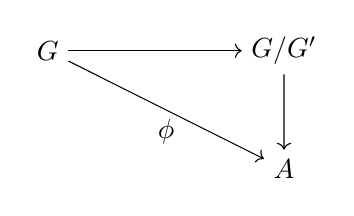
\begin{tikzpicture}[scale = 1.5]
                \node (G) at (0, 0) {$G$};
                \node (GG) at (2, 0) {$G/G'$};
                \node (A) at (2, -1) {$A$};

                \draw[->] (G) to (GG);
                \draw[->] (GG) to (A);
                \draw[->] (G) to node [below] {$\phi$} (A);
            \end{tikzpicture}
        \end{center}
    \end{enumerate}
\end{prop}

\begin{proofnum}
    \item Follows from the definition of the commutator.
    \item Observe that $H \nsub G$ if and only if $g\inv hg \in H$ for all $h \in H$ and $g \in G$. Similarly, for some $h \in H$, then $g\inv hg \in H$ if and only if $h\inv g\inv hg \in H$ so that $H \nsub G$ if and only if $[h, g] \in H$ for every $h \in H$ and $g \in G$. Hence, $H \nsub G$ if and only if $[H, G] \leq H$.
    \item For any $\sigma \in \aut(G)$ with $x, y \in G$, then
    \[\sigma([x, y]) = \sigma(x\inv y\inv xy) = \sigma(x)\inv \sigma(y)\inv \sigma(x)\sigma(y) = [\sigma(x), \sigma(y)].\]
    Hence, $G' = \gen{[x, y] \mid x, y \in G}$ is invariant under $\aut(G)$, so $G' \cha G$. Moreover, for any $x, y \in G$, we have
    \[(xG') (yG') = xyG' = yx[x, y]G' = yxG' = (yG')(xG').\]
    Hence, $G/G'$ is abelian.
    \item If $H \nsub G$ and $G/H$ is abelian, we have that $(xH)(yH) = (yH)(xH)$ for any $x, y \in G$. Then
    \[1H = (xH)\inv (yH)\inv (xH)(yH) = [x, y]H,\]
    so that $[x, y] \in H$ for every $x, y \in G$, and $G' \leq H$.

    If $G' \leq H$, then every subgroup of $G/G'$ is normal because $G/G'$ is abelian by the previous part. In particular, $H/G' \nsub G/G'$, so $H \nsub G$ by the Lattice Isomorphism Theorem. By the Third Isomorphism Theorem, we have
    \[G/H \cong (G/G')/(H/G')\]
    which is abelian since $G/G'$ is abelian.
    \item Similar to (4), we have $G' \leq \ker\phi$ since $\phi([x, y]) = [\phi(x), \phi(y)] = 1$ for all $x, y \in G$. Hence, $\phi$ factors through $G'$, and the diagram commutes.
\end{proofnum}

\begin{ex}[Examples of Commutators and Commutator Subgroups]
    \begin{itemize}
        \item $G$ is abelian if and only if $G' = 1$.
        \item Commutator subgroups can be computed without knowing all calculated commutators. For example, consider $G = D_8$ with $Z(D_8) = \gen{r^2} \nsub D_8$. Then $D_8/Z(D_8)$ is abelian, so $D_8' \leq Z(D_8)$. Since $[r, s] = r\inv s\inv rs = r^2$, we have $D_8' = Z(D_8) = \gen{r^2}$. In particular, a nonabelian group $G$ with order $p^3$ for prime $p$ has commutator subgroup of order $p$, and $G' = Z(G)$.
        \item Let $D_{2n}$ have usual presentation. Since $[r, s] = r^{-2}$, then $\gen{r^{-2}} = \gen{r^2} \leq D'_{2n}$. Moreover, $\gen{r^2} \nsub D_{2n}$ with the images of $r$ and $s$ in $D_{2n}/\gen{r^2}$ generate the quotient. Since they are commuting elements of order $\leq 2$, then the quotient is abelian, and $D'_{2n} \leq \gen{r^2}$. Hence, $D'_{2n} = \gen{r^2}$.
        
        If $n$ is odd, then $\gen{r^2} = \gen r$, whereas even $n$ implies $\gen{r^2}$ has index 2 in $\gen r$. Hence, $D'_{2n}$ is of index 2 or 4 in $D_{2n}$ depending on the parity of $n$.
        \item Since conjugation by $g \in G$ is in $\aut(G)$, then $[a^g, b^g] = [a, b]^g$ for all $a, b \in G$ by \autoref{prop5.7}(3),or conjugates of commutators are also commutators.
        
        As an example in $S_n$, deducing the cycle type of a commutator implies that every element of the same cycle type is also a commutator. In $S_5$, we know that every 5-cycle is a commutator: if we label the vertices of a pentagon as $1, 2, 3, 4, 5$, then $D_{10} \leq S_5$. Then the preceding exercises shows that an element of order 5 is a commmutator in $D_{10}$, so every 5-cycle is a commutator in $S_5$.
    \end{itemize}
\end{ex}

\begin{prop}[Decomposition in Subgroup Products]
    \label{prop5.8}
    Let $H$ and $K$ be subgroups of the group $G$. The number of distinct ways of writing each element of the set $HK$ in the form $hk$ for some $h \in H$ and $k \in K$ is $|H \cap K|$. In particular, if $H \cap K = 1$, then each element of $HK$ can be written uniquely as a product $hk$ for some $h \in H$ and $k \in K$. (This follows from \autoref{prop3.13}).
\end{prop}

\begin{proof}
    Let $x \in HK$. Then $x = h_1k_1$ for some $h_1 \in H$ and $k_1 \in K$. If $x = h_2k_2$ for some $h_2 \in H$ and $k_2 \in K$, then
    \[h_1\inv h_2 = k_1 k_2\inv.\]
    Since the left-hand side is in $H$ and the right-hand side is in $K$, we have that $h_1\inv h_2 \in H \cap K$. Conversely, if $h \in H \cap K$, then
    \[x = h_1 k_1 = (h_1 h) (h\inv k_1) = h_2 k_2\]
    where $h_2 = h_1 h \in H$ and $k_2 = h\inv k_1 \in K$. Hence, there are exactly $|H \cap K|$ distinct ways of writing each element of $HK$ in the form $hk$ for some $h \in H$ and $k \in K$. In particular, if $H \cap K = 1$, then each element of $HK$ can be written uniquely as a product $hk$ for some $h \in H$ and $k \in K$.
\end{proof}

\begin{theo}[Direct Product Recognition Theorem]
    \label{theo5.9}
    Let $G$ be a group with subgroups $H$ and $K$ such that
    \begin{enumerate}
        \item $H \nsub G$ and $K \nsub G$,
        \item $H \cap K = 1$.
    \end{enumerate}
    Then $HK \cong H \times K$.
\end{theo}

\begin{proof}
    By \autoref{cor3.15}, then $HK \leq G$. For $h \in H$ and $k \in K$, observe that normality of $H$ in $G$ implies that $k\inv hk \in H$, so $h\inv k\inv hk \in H$. Similarly, normality of $K$ in $G$ implies that $(h\inv k\inv h)k \in K$. Because $H \cap K = 1$, then $h\inv k\inv hk = 1$, or $hk = kh$ so that $H$ and $K$ commute elementwise. By \autoref{prop5.8}, elements of $H$k are uniquely written as a product $hk$ for $h \in H$ and $k \in K$. Then
    \[\phi : HK \to H \times K \quad \text{defined by} \quad \phi(hk) = (h, k)\]
    is well-defined. Moreover, $\phi$ is a homomorphism since for any $h_1, h_2 \in H$ and $k_1, k_2 \in K$, we have
    \[\phi((h_1k_1)(h_2k_2)) = \phi(h_1 h_2 k_1 k_2) = (h_1 h_2, k_1 k_2) = (h_1, k_1)(h_2, k_2) = \phi(h_1k_1)\phi(h_2k_2).\]
    Finally, $\phi$ is bijective because each $hk$ is uniquely written. Hence, $\phi$ is an isomorphism, and $HK \cong H \times K$.
\end{proof}

\begin{ex}[Examples of Internal Direct Products]
    \begin{enumerate}
        \item Let $n$ be positive and odd. Then $D_{4n} \cong D_{2n} \times Z_2$. Let
        \[D_{4n} = \gen{r, s \mid r^{2n} = s^2 = 1, srs = r\inv}.\]
        Let $H = \gen{s, r^2}$ and $K = \gen{r^n}$. Since $H$ has index 2 (because $H$ contains $s$ and $r^2$ but not $r$), then $H \nsub D_{4n}$. Note that both $s$ and $r$ centralize $r^n$, so $K \leq Z(D_{4n})$, hence $K \nsub D_{4n}$. Note that $K \not\leq H$ since $r^n \notin H$, so $H \cap K = 1$. By \autoref{theo5.9}, then $D_{4n} = HK \cong H \times K$. Since $H$ is generated by an element of order 2 and an element of order $n$ that commute, then $H \cong D_{2n}$, and $K \cong Z_2$. Hence, $D_{4n} \cong D_{2n} \times Z_2$.
        \item Let $I \subseteq \set{1, 2, \ldots, n}$ and $G$ be the setwise stabilizer of $I$ in $S_n$, i.e.,
        \[G = \set{\sigma \in S_n \mid \sigma(i) \in I \text{ for all } i \in I}.\]
        Let $J = \set{1, 2, \ldots, n} \setminus I$. Note that $G$ is also the setwise stabilizer of $J$ in $S_n$. Let $H$ and $K$ be the pointwise stabilizers of $I$ and $J$ in $S_n$, respectively, i.e.,
        \[H = \set{\sigma \in S_n \mid \sigma(i) = i \text{ for all } i \in I}\]
        and
        \[K = \set{\sigma \in S_n \mid \sigma(j) = j \text{ for all } j \in J}.\]
        To see that $H$ and $K$ are normal in $G$, note that if $G$ acts on $I$ and $J$ by permuting the elements, then $H$ and $K$ are the kernels of these actions, so $H$ and $K$ are normal in $G$. Moreover, $H \cap K = 1$ since if $\sigma \in H \cap K$, then $\sigma(i) = i$ for all $i \in I$ and $\sigma(j) = j$ for all $j \in J$, so $\sigma = 1$. By \autoref{theo5.9}, then $G = HK \cong H \times K$. Since $H$ is isomorphic to a subgroup of $S_{n - |I|}$ and $K$ is isomorphic to a subgroup of $S_{|I|}$, then $G \cong S_{n - |I|} \times S_{|I|}$.
        \item Let $\sigma \in S_n$, and let $I$ be the subset of $\set{1, 2, \ldots, n}$ fixed by $\sigma$ pointwise:
        \[I = \set{i \in \set{1, 2, \ldots, n} \mid \sigma(i) = i}.\]
        Let $C = C_{S_n}(\sigma)$. Using Exercise 4.3.18, then $C$ stabilizes $I$ and its complement $J$. Then $C$ is isomorphic to a subgroup $H \times K$, where $H$ is a subgroup of $S_{n - |I|}$ and $K$ is a subgroup of $S_{|I|}$. Noting that $\sigma \in H$, we argue by the preceding example that any $\alpha \in C$ can be written uniquely as $\alpha = \alpha_I\alpha_J$ where $\alpha_I \in H$ and $\alpha_J \in K$. For any $\tau$ that fixes $j \in J$, then $\sigma$ and $\tau$ commute. Then $C$ contains all such $\tau$, or the subgroup $K$. Then $C$ indeed is the set of elements $\alpha_I\alpha_J \in H \times K$ with arbitrary $\alpha_J \in K$ and $\alpha_I$ commutes with $\sigma$:
        \[C = C_H(\sigma) \times K \cong C_{S_J}(\sigma) \times S_I.\]
        In particular, if $\sigma$ is an $m$-cycle, then
        \[C_{S_n}(\sigma) \cong \langle \sigma \rangle \times S_{n-m}.\]
        This has order $m(n - m)!$.
    \end{enumerate}
\end{ex}

\newpage

\subsection{Semidirect Products}

\begin{defn}
    \item Let $H$ and $K$ be groups, and let $\phi : K \to \aut(H)$ be a homomorphism. The \textbf{semidirect product} of $H$ and $K$ with respect to $\phi$ is the group $H \semidir_\phi K$. If the homomorphism $\phi$ is clear from the context, then we simply write $H \semidir K$.
    \item The \textbf{generalized quaternion group of order $2^{n + 1}$} is the group
    \[Q_{2^{n + 1}} = \gen{h, x \mid h^{2^n} = x^4 = 1, x\inv hx = h\inv, h^{2^{n - 1}} = x^2}\]
    for $n \geq 2$.
    \item Let $H$ be a group with $K = \aut(H)$, and $\phi = \id$. Then the semidirect product $H \semidir_\phi K$ is called the \textbf{holomorph} of $H$, denoted $\hol(H)$.
\end{defn}

\begin{theo}[Semidirect Product Construction]
    \label{theo5.10}
    Let $H$ and $K$ be groups, and let $\phi : K \to \aut(H)$ be a homomorphism. Let $\cdot$ be the action of $K$ on $H$ determined by $\phi$. Let $G$ be the set of ordered pairs $(h, k)$ with $h \in H$ and $k \in K$ with the defined multiplication:
    \[(h_1, k_1)(h_2, k_2) = (h_1 (k_1 \cdot h_2), k_1 k_2).\]
    \begin{enumerate}
        \item $G$ is a group with order $|H||K|$.
        \item The sets $\set{(h, 1) \mid h \in H}$ and $\set{(1, k) \mid k \in K}$ are subgroups of $G$ isomorphic to $H$ and $K$ via the maps $h \mapsto (h, 1)$ and $k \mapsto (1, k)$, respectively. We identify these subgroups with $H$ and $K$, or
        \[H \cong \set{(h, 1) \mid h \in H}, \quad K \cong \set{(1, k) \mid k \in K}.\]
    \end{enumerate}
    Upon identification in $G$, we have the following properties:
    \begin{enumerate}[resume]
        \item $H \nsub G$,
        \item $H \cap K = 1$,
        \item for all $h \in H$ and $k \in K$, then $khk\inv = k \cdot h = \phi(k)(h)$.
    \end{enumerate}
\end{theo}

\begin{proofnum}
    \item To see that $G$ is a group, we verify the group axioms:
    \begin{itemize}
        \item Closure: For any $(h_1, k_1), (h_2, k_2) \in G$, then $h_1 (k_1 \cdot h_2) \in H$ and $k_1 k_2 \in K$, so $(h_1 (k_1 \cdot h_2), k_1 k_2) \in G$.
        \item Associativity: For any $(h_1, k_1), (h_2, k_2), (h_3, k_3) \in G$, then
        \begin{align*}
            ((h_1, k_1)(h_2, k_2))(h_3, k_3) &= (h_1 (k_1 \cdot h_2), k_1 k_2)(h_3, k_3) \\
            &= ((h_1 (k_1 \cdot h_2)) ((k_1 k_2) \cdot h_3), (k_1 k_2) k_3) \\
            &= (h_1 ((k_1 \cdot h_2) ((k_1 k_2) \cdot h_3)), k_1 (k_2 k_3)) \\
            &= (h_1 ((k_1 \cdot h_2) (k_1 \cdot (k_2 \cdot h_3))), k_1 (k_2 k_3)) \\
            &= (h_1 (k_1 \cdot (h_2 (k_2 \cdot h_3))), k_1 (k_2 k_3)) \\
            &= (h_1, k_1)((h_2, k_2)(h_3, k_3))
        \end{align*}
        where the fourth equality follows from the definition of a group action.
        \item Identity: $(1, 1)$ is the identity element of $G$ since for any $(h, k) \in G$, then
        \[(1, 1)(h, k) = (1 (1 \cdot h), 1 k) = (h, k)\]
        and
        \[(h, k)(1, 1) = (h (k \cdot 1), k 1) = (h, k).\]
        \item Inverses: For any $(h, k) \in G$, then
        \[(h, k)(k\inv \cdot h\inv, k\inv) = (h (k \cdot (k\inv \cdot h\inv)), k k\inv) = (h h\inv, 1) = (1, 1)\]
        and
        \[(k\inv \cdot h\inv, k\inv)(h, k) = ((k\inv \cdot h\inv) (k\inv \cdot h), k\inv k) = (1, 1).\]
        Hence, $(h, k)\inv = (k\inv \cdot h\inv, k\inv)$.
    \end{itemize}
    \item Let $\wt H = \set{(h, 1) \mid h \in H}$ and $\wt K = \set{(1, k) \mid k \in K}$. Observe that $\wt H$ and $\wt K$ are subgroups of $G$ since for any $h_1, h_2 \in H$ and $k_1, k_2 \in K$, then
    \[(h_1, 1)(h_2, 1) = (h_1 h_2, 1) \in \wt H\]
    and
    \[(1, k_1)(1, k_2) = (1, k_1 k_2) \in \wt K.\]
    Moreover, the maps $h \mapsto (h, 1)$ and $k \mapsto (1, k)$ are isomorphisms since they are bijective homomorphisms. Hence, $\wt H$ and $\wt K$ are subgroups of $G$ isomorphic to $H$ and $K$.
    \item Under the identification of $\wt H$ and $\wt K$ with $H$ and $K$, we see that $K \leq N_G(H)$ since for any $h \in H$ and $k \in K$, then
    \[k\inv hk = (1, k)\inv (h, 1)(1, k) = (k\inv \cdot h, 1) \in H.\]
    Hence, $H \nsub G$.
    \item It is clear that $\wt H \cap \wt K = 1$, so $H \cap K = 1$ under the identification.
    \item For $(1, k) \in \wt K$ and $(h, 1) \in \wt H$, then
    \[(1, k)(h, 1)(1, k)\inv = (1, k)(h, 1)(k\inv \cdot 1, k\inv) = (k \cdot h, 1)\]
    so that $khk\inv = k \cdot h = \phi(k)(h)$ under the identification.
\end{proofnum}

\begin{prop}[Criterion for Equivalence of Semidirect and Direct Products]
    \label{prop5.11}
    Let $H$ and $K$ be groups, and let $\phi : K \to \aut(H)$ be a homomorphism. Then the following are equivalent:
    \begin{enumerate}
        \item The identity (set) map between $H \semidir K$ and $H \times K$ is a group homomorphism, or $H \semidir K \cong H \times K$.
        \item $\phi$ is the trivial homomorphism, i.e., $\phi(k) = 1$ for all $k \in K$,
        \item $K \nsub H \semidir K$.
    \end{enumerate}
\end{prop}

\begin{proof}
    \leavevmode\newline
    $(1) \Rightarrow (2)$: By definition for $h_1, h_2 \in H$ and $k_1, k_2 \in K$ in $H \semidir K$, we have
    \[(h_1, k_1)(h_2, k_2) = (h_1 (k_1 \cdot h_2), k_1 k_2)\]
    If the identity map is a homomorphism, then $(h_1, k_1)(h_2, k_2) = (h_1 h_2, k_1 k_2)$ in $H \times K$. Hence, $h_1 (k_1 \cdot h_2) = h_1 h_2$ for all $h_1, h_2 \in H$ and $k_1 \in K$, so $\phi(k) = 1$ for all $k \in K$.

    \noindent $(2) \Rightarrow (3)$: If $\phi$ is trivial, then the action of $K$ on $H$ is trivial, so the multiplication in $H \semidir K$ is given by
    \[(h_1, k_1)(h_2, k_2) = (h_1 h_2, k_1 k_2)\]
    so that $H \semidir K = H \times K$. Since $K \nsub H \times K$, then $K \nsub H \semidir K$.

    \noindent $(3) \Rightarrow (1)$: If $K \nsub H \semidir K$, then (referencing \autoref{theo5.9}) for all $h \in H$ and $k \in K$, we have $[h, k] \in H \cap K = 1$. Then $kh = hk$, so the action of $K$ on $H$ is trivial, or $\phi(k) = 1$ for all $k \in K$. Hence, the multiplication in $H \semidir K$ is given by
    \[(h_1, k_1)(h_2, k_2) = (h_1 h_2, k_1 k_2)\]
    so that $H \semidir K = H \times K$.
\end{proof}

\begin{ex}[Examples of Semidirect Products]
    Let $H$ and $K$ be groups with homomorphism $\phi : K \to \aut(H)$. Let $G = H \semidir K$, and identify $H$ and $K$ as subgroups of $G$ as in \autoref{theo5.10}(2). We will use \autoref{prop4.16} and \autoref{prop4.17} to determine homomorphisms $\phi$ for specific $H$. The proofs for showing $\phi$ is a homomorphism are omitted, since $K$ will often by cyclic.
    \begin{enumerate}
        \item Let $H$ be abelian (and positively infinite), and let $K = \gen x \cong Z_2$. Define $\phi : K \to \aut(H)$ that maps $x$ to the inverting automorphism of $H$ so that $x \cdot h = h\inv$ for every $h \in H$. Then $G$ contains $H$ as a normal subgroup of index 2, and
        \[xhx\inv = h\inv \quad \text{for all $h \in H$.}\]
        When $H = Z_n$, then $G \cong D_{2n}$, the dihedral group of order $2n$. If $H = \gen z$, then $G = D_\infty$, the infinite dihedral group.
        \item Generalizing the previous example, let $H$ be abelian and $K = \gen x \cong Z_{2n}$. Using the same $\phi$ as before, then $x^2$ acts trivially on $H$. In $G$, we have $xhx\inv = h\inv$, and $x^2hx^{-2} = h$ for all $h \in H$. Then $x^2 \in Z(G)$. If we take $H = Z_3$ and $K = Z_4$, then $G$ is non-abelian of order 12 that is not isomorphic to $A_4$ or $D_{12}$ because its Sylow-2 subgroup, $K$, is cyclic of order 4.
        \item Another generalization of (1) is to let $H = \gen H \cong Z_{2^n}$, $K = \gen x \cong Z_4$ with $xhx\inv = h\inv$. By above, $x^2 \in Z(G)$, and $x$ inverting $H$ implies that $x$ inverts $\gen z$, where $z = h^{2^{n - 1}}$. Then $xzx\inv = z\inv = z$, so $z \in Z(G)$. Then $x^2z \in Z(G)$, or $\gen{x^2z} \nsub G$.
        
        Let $\bar G = G/\gen{x^2z}$. Because $x^2$ and $z$ are distinct commuting elements of order 2, then $|x^2z| = 2$, hence $|\bar G| = 2^{n + 1}$. By factoring out $x^2z$, which implies $x^2 = z\inv = z$, then we may identify $x^2$ and $h^{2^{n - 1}}$ in $\bar G$. For $n = 2$, this implies that $\bar x$ and $\bar h$ are elements of order 4. To see this, suppose $\bar x^2 = 1$. Then $x^2 \in \gen{x^2z}$, so $x^2 = x^2z$ or $x^2 = 1$. Since $z \neq 1$, and $|x| = 4$, this cannot hold. To see that $|\bar h|= 4$, we note that its order divides 4, and $\bar h^2 = \bar x^2 \neq 1$, so its order is 4. We also have that $\bar x$ inverts $\bar h$, and $\bar h^2 = \bar x^2$ is central in $\bar G$. Then $\bar G$ satisfies the same presentation as $Q_8$, so $\bar G \cong Q_8$.

        Suppose $n > 2$. We show that $\bar G$ has a unique subgroup of order 2, namely $\gen{\bar x^2}$. Let $\bar h^i \bar x^j$ be an element in $\bar G$. We split into three cases:
        \begin{itemize}
            \item If $j = 0$, then $\bar h^i$ has order 2 if and only if $\bar h^i = \bar h^{2^{n - 1}} = \bar x^2$.
            \item If $j = 2$, then $(\bar h^i\bar x^2)^2 = \bar h^{2i}$ has order 2 if and only if $\bar h^{2i} = \bar h^{2^{n - 1}} = \bar x^2$, hence $\bar h^i\bar x^2$ has order 4.
            \item If $j = 1$ or $3$, then $\bar x^j$ inverts $\bar h$, so $(\bar h^i \bar x^j)^2 = \bar h^i \bar x^j \bar h^i \bar x^j = \bar h^i (\bar x^j \bar h^i \bar x^{-j}) \bar x^{2j} = \bar h^i \bar h^{-i}\bar x^{2j} = \bar x^2$, so $\bar h^i \bar x^j$ has order 4.
        \end{itemize}

        We claim that $Z(\bar G) = \gen{\bar x^2}$. To see that $\bar x^2 \in Z(\bar G)$, recall that $\bar x^2 = \bar h^{2^{n - 1}}$. This commutes with $\bar h$ trivially, while $\bar x^2$ clearly commutes with $\bar x$. We call $\bar G$ the \textbf{generalized quaternion group} of order $2^{n + 1}$, which is denoted by $Q_{2^{n + 1}}$ with the presentation:
        \[Q_{2^{n + 1}} = \gen{h, x \mid h^{2^n} = x^4 = 1, x\inv hx = h\inv, h^{2^{n - 1}} = x^2}\]
            \item Let $H = (\q, +)$ and $K = \gen x \cong \z$. Let $\phi$ be the map of multiplying by 2 on $H$, hence $x \cdot h = 2h$ for every $h \in H$. Note that $x \z x\inv = 2\z \subset \z$, but $2z \neq \z$, hence $x \not\in N_G(\z)$. This shows that containment is not enough to guarantee normality. 
        \item The semidirect $H \semidir \aut(H)$ is called the \textbf{holomorph} of $H$, denoted $\hol(H)$. Some common holomorphs are:
        \begin{itemize}
            \item $\hol(Z_2 \times Z_2) \cong S_4$,
            \item Let $|G| = n$ and $\pi : G \to S_n$ be the left regular representation. Then $N_{S_n}(\pi(G)) \cong \hol(G)$. Note that the left regular reprsentation of a generator of $Z_n$ is an $n$-cycle in $S_n$, hence
            \[N_{S_n}(\gen{(1\, 2 \ldots n)}) \cong \hol(Z_n) = Z_n \semidir \aut(Z_n)\]
        \end{itemize}
        \item 
    \end{enumerate}
\end{ex}

\end{document}